\chapter{Reasoning about Metric-Timed Normative Conflicts}

\section{Overview}
\label{sec:overview}

Normative systems provide the formal backbone for how organizations, individuals, software, and autonomous agents are expected to behave. A \emph{normative specification} describes these expectations as a set of rules determining what an agent ought to do or what state of affairs ought to be. However, dealing with such specifications is inherently difficult. They combine different types of rules, such as obligations, prohibitions, and permissions, whose interplay can yield overlapping prescriptions. In many situations, complying with one norm causes the violation of another. This situation is referred to as a \emph{normative conflict}.

Intuitively, conflicts arise when norms are defined that cannot be jointly fulfilled by an agent. Detecting these disputes is essential. In law, undetected incompatibilities threaten legal certainty. In regulatory frameworks, they undermine enforceability and make automated compliance checking unreliable. Furthermore, reinforcement learning is increasingly used to enforce compliant behavior in agent planning tasks \cite{neufeld2025combining,neufeld2022enforcing}. When the underlying normative specification contains conflicts, the induced reward signal becomes internally inconsistent, causing agents to learn oscillatory behaviors or arbitrary preferences. Therefore, any formal method aiming to support normative reasoning must explicitly expose these issues and eliminate them before a reward model is derived.

\subsection{Motivation}

This chapter studies conflicts in \emph{ought-to-do} specifications with explicit temporal conditions. While untimed conflicts are well understood, time plays a central role in complex specifications. Norms are rarely timeless; they are activated, suspended, or expire under explicit conditions. This temporal structure has motivated research in two distinct traditions:

\begin{enumerate}
    \item \textbf{Deontic Logic:} This field offers rich treatments of norms, exceptions, and legal dynamics \cite{makinson2000input,governatori2011justice}. However, the treatment of time is often syntactic, relying on triggers or deadlines rather than a semantic interpretation of time. Consequently, these logics seldom deliver constructive, punctual diagnoses or calculi for equivalence-preserving repairs.
    \item \textbf{Formal Verification:} Communities using Linear Temporal Logic (LTL) or Metric Interval Temporal Logic (MITL) treat time as a first-class semantic component \cite{alur1996benefits}. However, the focus here is typically on \emph{satisfiability} (does a model exist?) rather than \emph{conflict} (do two rules clash?). Existing SMT-based diagnostics \cite{10.1145/3597503.3639093} can identify unsatisfiable cores but often ignore the ontic feasibility of agents (what an agent can actually perform).
\end{enumerate}

\paragraph{The Gap}
A conceptual gap remains between these traditions. We lack a framework that internalizes metric time as a semantic constraint on actions while providing precise definitions for conflicts linked to specific time points. Unlike in untimed settings, conflicts in timed specifications constitute a scheduling and capacity problem. They depend on \emph{when} norms are active and \emph{how many} are active simultaneously. A specification might be logically consistent in the abstract yet impossible to fulfill because an agent cannot physically perform the required actions within the specified interval sets.

We address this by focusing on \emph{temporal infeasibility} under specific \emph{ontic conditions}. We assume discrete time and punctual actions where an agent is subject to a single-action constraint: at any time point, the agent performs at most one action. This aligns compliance checking with scheduling, allowing us to analyze conflicts not just as logical contradictions ($O\alpha \land O\lnot\alpha$) but as the impossibility of a feasible schedule.

\subsection{Methodology}

To address these challenges, we formalize the potential behavior of agents as finite timed words. We introduce a logic, $\TDDLfm$, allowing us to formalize normative specifications where time conditions are represented as finite interval sets. This trace-based semantics serves as the ground truth for our analysis.

Our approach relies on characterizing conflicts as a syntactic property that coincides with semantic unsatisfiability. We identify two elementary types of conflicts that occur at exact instants:
\begin{itemize}
    \item \textbf{Deontic conflicts:} An agent is simultaneously obliged and prohibited to perform the same action.
    \item \textbf{Ontic conflicts:} Multiple obligations require different actions at the same time, but the agent can realize at most one.
\end{itemize}

These punctual conflicts constitute the atomic sources of unsatisfiability. To expose them, we introduce a normal form for our specifications: the \emph{Disjunctive Punctual Normal Form} (\dpnf). This transformation allows us to use ideas similar to unsat cores in SMT but adapted for normative structures. Because conflict is a syntactic property, we must ensure that translating a given specification into our normal form neither introduces nor removes conflicts. To this end, we identify and prove properties of syntactic transformations, specifically the \emph{Lowest Upper Common Operator} (\LUCO) and \emph{Literal Ancestor Preservation} (\LAP), which guarantee that the presence of a conflict is unaltered during normalization.

Using this machinery, we demonstrate that our definition of conflicts coincides with the notion of Minimal Unsatisfiable Subsets (MUS). This establishes that unsatisfiability in our logic can be completely explained through these two conflict patterns.

\subsection{Contribution}

In this chapter, we provide a logical framework for \emph{metric-time normative conflicts} that deals with these issues in a mathematically precise manner. Our specific contributions are as follows:

\begin{itemize}
    \item \textbf{Formal Machinery:} We define a compact, action-based logic over finite interval sets. We provide algorithms for punctual and disjunctive normalization (\dpnf) and a proof-theoretic calculus for conflict detection.
    
    \item \textbf{Conflict Characterization:} We offer precise definitions for conflicts and conditions for their correct detection. We prove that deontic and ontic conflicts correspond precisely to Minimal Unsatisfiable Subsets (MUS) in our logic. Conversely, we show that any MUS is necessarily an instance of one of these conflict types.
    
    \item \textbf{Quantitative Metrics:} We introduce the concept of \emph{conflict density}, which measures the ratio of conflicting to total punctual obligations. We show that a conflict density of 1 implies unsatisfiability, while a density below 1 allows for a conflict-free, semantics-preserving pruning.
    
    \item \textbf{Elimination and Guarantees:} We provide sound and complete methods for equivalence-preserving conflict elimination. We analyze the verbosity induced by this process, demonstrating that while eliminating conflicts can increase the syntactic size of the specification, the blow-up remains bounded under well-defined structural conditions.
\end{itemize}

Altogether, this framework allows us to identify conflicts in a specification, explain their causes via interval arithmetic, measure their density, and eliminate them without altering the intended compliant behaviors.
\section{Use Case: Goods Delivery Contract}\label{sec:usecase}


Our use case examines a contract between a trucking company and a harbor, focusing on the daily delivery of potentially hazardous goods to the harbor.  
%
Table~\ref{tab:contract} presents a portion of the contract signed between the trucking company and the harbor. For clarity, we do not provide the full contractual agreement, but instead highlight select sections to illustrate our language and the occurrence of \textit{potential conflicts}.


\newcolumntype{C}{>{\columncolor{lightgray}}p{0.8\textwidth}}

\begin{table}[h]

  \begin{tabular}{|C|r|}
  \hline 
  \dots     &  \\
  The deliveries \textit{shall} be made everyday to \textit{either the gate terminal or the designated parking area of the harbor}. The delivery must be done  \textit{between 09:00 to 16:00 }.
     & (\DC) \\
\dots & \\
    Delivery of dangerous goods to the harbor's parking lot is prohibited between 10:00 and 14:00.
& (\SR)\\   
\dots & \\
   When delivering goods, special restrictions may apply due to maintenance activity in the harbor. &  (\MC)\\
  \dots & \\
  \hline    
\end{tabular}
    \caption{Contract between trucking company and a harbor company}
    \label{tab:contract}
\end{table}


Let us elaborate on the contract. There are individuals and legal entities involved, like the truck driver, the transportation company and the harbor. 

The contract involves several clauses; first, a \emph{Delivery Clause} (\DC) for all goods. Moreover, there is a clause adding additional \emph{Safety Regulations} (\SR) when dangerous goods are involved. The third and final clause requires respecting any \emph{Maintenance Clause} (\MC) of the harbor when delivering goods. 


The Delivery Clause (\DC) specifies the designated delivery location and time frame (between 09:00 and 16:00)  to be performed on a daily basis; the harbor carries on by loading the goods onto the ferry on fixed and reserved slots as specified in the contract, making the driver's delivery act mandatory in the delivery chain. The Safety Regulation clause \SR prohibits the delivery of \emph{dangerous} goods in the harbor's parking area between 10:00 and 14:00. The Maintenance Clause \MC mandates compliance with announcements when delivering goods. These maintenance announcements are issued by the harbor's infrastructure management unit by providing a \emph{Maintenance Announcement} document (\MA) requiring consultation (cf.~the document shown in Tab.~\ref{tab:ma}). This document may be empty in case no announcement is in place or adds specific clauses. 


\begin{table}
    \centering
    \begin{tabular}{|C|c|}
    \hline
    Due to infrastructure damage at the harbor, the delivery of dangerous goods to the gate terminal is temporarily prohibited during the following hours: (1) Between 02:00 and 04:00, and (2) between 08:00 and 24:00. & (\MA)\\
    \hline
    \end{tabular}
    \caption{Maintenance Announcement}
    \label{tab:ma}
\end{table}


Let us now reconsider the contract and perform a more conceptual analysis: 
\conceptInOneWord{agent}%
Individuals and legal entities affected by the normative system are called \emph{agents}. These agents are required to follow the prescriptions and rules of the contract or agreement, which are collectively termed \emph{norms}. In this paper, we focus on formalizing norms concerning a \emph{single} agent, leaving multi-agent scenarios for future work. 
\conceptInOneWord{norms}%
Norms stipulate what the different agents are permitted, obliged or forbidden to do, as well as the penalties to be applied in case of non-compliance. As explained in the introduction, we focus here not on \emph{full} normative systems but on a subset of normative statements.
%
%In this paper, we focus on formalizing the norms that a single agent must adhere to, leaving multi-agent scenarios for future work. Importantly, an agent is not bound by just one norm but must comply with several norms simultaneously. These norms pertain to specific \emph{time points}, which we represent as natural numbers. More precisely, norms are associated with time \emph{intervals}, and the agent must adhere to constraints across multiple such intervals. Therefore, we need to define intervals and establish operations for \emph{interval arithmetic}.
% In this paper, we focus on formalizing norms concerning a \emph{single} agent, leaving multi-agent scenarios for future work. 
\conceptInOneWord{norms distributed}%
An agent is typically not bound by just one norm but must comply with several norms simultaneously (all the norms in the given normative system(s) under consideration). The norms may be distributed over several documents.
%
\conceptInOneWord{time}%
The norms are enacted (and enforced) at specific \emph{time points}. In general, such time points are explicitly or implicitly written in the contract and they can be expressed in relative or absolute time. For instance, they can be relative to a certain date (e.g., when the contract was signed) or to the occurrence of certain events, or then expressed as dates, hours of a day, etc. Without loss of generality, we represent such time points as natural numbers.\footnote{It is always possible to convert from relative to absolute time (and vice-versa) as well as to map hours and dates into natural numbers.} More precisely, norms are associated with time \emph{intervals}, and the agent must adhere to constraints across multiple such intervals. In the next section, we will make these notions more formal (e.g., we will define intervals and establish operations for \emph{interval arithmetic}).

%The driver's task is to deliver goods within specific time constraints defined by these intervals. Thus, she must perform specific \emph{actions} at designated times. When the driver acts, their behavior can be observed as \emph{timed action sequences}, which we model as timed words.
\conceptInOneWord{actions}%
Back to our use case, the driver's task is to deliver goods within specific time constraints defined as intervals as stipulated in the contract. Whenever the driver performs \emph{actions} which are within the scope of the contract, we may consider that the contract is being \emph{executed}. Such actions happen at a given time point. We thus represent the sequence of actions (the behavior of the agent) as \emph{timed action sequences}, which are modeled as \emph{\timedwords}. We simplify our framework by assuming that each action is instantaneous and happens at a single point in time. Actions with longer durations may be considered in future work.

\conceptInOneWord{detailed analysis}
With this framework in place, we now proceed to a more detailed analysis of the normative specifications of our use case. First, we can identify the following two actions to be performed by the driver:
% \begin{enumerate}
%     \item Delivery at the gate (\delAtGate), present in \DC and \MA.
%     \item Delivery at the parking (\delAtPark), present in \DC and \SR.
% \end{enumerate}
\begin{enumerate}
    \item Delivery at the gate, denoted by \delAtGate, cf.~\DC and \MA;
    \item Delivery at the parking, denoted by \delAtPark, cf.~\DC and \SR.
\end{enumerate}
%
% \todo[inline]{You use the font \delAtGate for many of the actions. The font becomes ``invisible'' in the text. Use another font for all actions in a uniform way (and consistent with how you use the fonts for other things). E.g., \texttt{\delAtGate} or other font. [Gerardo]\\
% I am using \"mtext" macros which is reconfigurable as we want, I switched to mathsf for now, let me know if it still needs to be changed [KK]}
%
% The identified  actions are subject to \textit{obligations} (requirement of acting) and \emph{prohibitions} (requirement of not performing  the actions): 
% \begin{enumerate}
%     \item Obligation: \delAtGate and \delAtPark are obliged in \DC as specified by the word \textit{shall}.
%     \item Prohibition: \delAtGate is prohibited in \MA and \delAtPark is prohibited in \SR.
% \end{enumerate}
% Both actions are subject to obligations and prohibition. Furthermore, timed constraints are additionally prescribed for the obligations and prohibitions from the three normative systems:
% \begin{enumerate}
% \item \textit{Between 09:00 and 16:00}: concerning the obligation \delAtPark found in \DC.
% \item \textit{Between 10:00 and 14:00}: concerning the prohibition on \delAtPark found in \SR.
% \item \textit{Between 02:00 and 04:00 and between 08:00 and 24:00} concerning the prohibition on \delAtGate found in \MA.
% \end{enumerate}
The identified driver's actions are subject to \textit{obligation: has to perform the action} and \emph{prohibition: has to abstain from performing the action}: 
\begin{enumerate}
    \item Obligation: \delAtGate and \delAtPark, cf.~\DC;
    \item Prohibition: \delAtGate, cf.~\MA, and \delAtPark, cf.~\SR.
\end{enumerate}
The obligations and prohibitions are to be enacted on specific intervals of time:
%
\begin{enumerate}
\item \textit{Between 09:00 and 16:00}: concerning the obligation on \delAtPark, cf.~\DC
\item \textit{Between 10:00 and 14:00}: concerning the prohibition on \delAtPark, cf.~\SR
\item \textit{Between 02:00 and 04:00 and between 08:00 and 24:00} concerning the prohibition on \delAtGate, cf.~\MA
\end{enumerate}



 \begin{figure}
\begin{center}
\begin{tikzpicture}[scale=0.8,transform shape]
  % Hour mapping: 1h = 0.5cm, shifted +1cm
  \begin{scope}[x=0.5cm, shift={(1cm,0)}]

    % Layout parameters
    \def\laneH{0.45}      % thinner rectangles
    \def\offset{0.25}     % vertical offset for obligation band
    \def\yshiftText{0.6}  % downward shift for prohibition text
    \def\rectShift{0.3}   % upward shift of rectangles
    \def\ygate{1.6}
    \def\ypark{-1.6}

    % Styles
    \tikzset{
      obl/.style ={
        draw=blue!80!black, line width=0.8pt, rounded corners=2pt,
        pattern={Lines[angle=45,distance=2pt,line width=0.3pt]},
        pattern color=blue!70!black, fill opacity=1
      },
      proh/.style={
        draw=red!80!black, line width=0.8pt, rounded corners=2pt,
        pattern={Lines[angle=90,distance=2pt,line width=0.3pt]},
        pattern color=red!80!black, fill opacity=1
      },
      tick/.style={gray!60, line width=0.4pt}
    }

    % ==== Timelines ====
    % Gate
    \draw[thick,->] (0,\ygate) -- (24.8,\ygate);
    % Dashes every 2 hours
    \foreach \t in {0,2,...,24} {
      \draw[tick] (\t,\ygate-0.12) -- (\t,\ygate+0.12);
    }
    % Hour labels
    \foreach \t in {0,2,4,6,8,10,12,14,16,18,20,22,24} {
      \node[below=3pt, font=\scriptsize] at (\t,\ygate) {\t:00};
    }

    % Park
    \draw[thick,->] (0,\ypark) -- (24.8,\ypark);
    % Dashes every 2 hours
    \foreach \t in {0,2,...,24} {
      \draw[tick] (\t,\ypark-0.12) -- (\t,\ypark+0.12);
    }
    % Hour labels
    \foreach \t in {0,2,4,6,8,10,12,14,16,18,20,22,24} {
      \node[below=3pt, font=\scriptsize] at (\t,\ypark) {\t:00};
    }

    % Labels for each action
    \node[anchor=east, font=\large] at (-0.8,\ygate+1) {Timeline for $\delAtGate$};
    \node[anchor=east, font=\large] at (-0.8,\ypark+1) {Timeline for $\delAtPark$};

    % ==== Intervals ====
    % Gate: prohibitions [2,4], [8,24]; obligation [9,16]
    \def\GateProhSmallA{2} \def\GateProhSmallB{4}
    \def\GateProhA{8}      \def\GateProhB{24}
    \def\GateOblA{9}       \def\GateOblB{16}
    % Park: obligation [9,16]; prohibition [10,14]
    \def\ParkOblA{9}   \def\ParkOblB{16}
    \def\ParkProhA{10} \def\ParkProhB{14}

    % ===== Gate rectangles =====
    % Prohibitions (red vertical lines)
    \path[proh] (\GateProhSmallA,\ygate+\rectShift-\laneH/2)
      rectangle (\GateProhSmallB,\ygate+\rectShift+\laneH/2);
    \path[proh] (\GateProhA,\ygate+\rectShift-\laneH/2)
      rectangle (\GateProhB,\ygate+\rectShift+\laneH/2);
    % Obligation (blue diagonal lines)
    \path[obl]  (\GateOblA,\ygate+\rectShift+\offset-\laneH/2)
      rectangle (\GateOblB,\ygate+\rectShift+\offset+\laneH/2);

    % Labels
    \node[blue!80!black, font=\small,yshift=+0.2cm]
      at ({(\GateOblA+\GateOblB)/2},\ygate+\rectShift+\offset+\laneH/1.3) {Obligation (DC)};
    \node[red!80!black, font=\small,yshift=1.5cm,xshift=1.5cm]
      at ({(\GateProhA+\GateProhB)/2},\ygate+\rectShift-\laneH/1.3-\yshiftText) {Prohibition (MA)};
    \node[red!80!black, font=\small,yshift=+1.5cm]
      at ({(\GateProhSmallA+\GateProhSmallB)/2},\ygate+\rectShift-\laneH/1.3-\yshiftText) {Prohibition (MA)};

    % ===== Park rectangles =====
    % Prohibition (red vertical lines)
    \path[proh] (\ParkProhA,\ypark+\rectShift-\laneH/2)
      rectangle (\ParkProhB,\ypark+\rectShift+\laneH/2);
    % Obligation (blue diagonal lines)
    \path[obl]  (\ParkOblA,\ypark+\rectShift+\offset-\laneH/2)
      rectangle (\ParkOblB,\ypark+\rectShift+\offset+\laneH/2);

    % Labels
    \node[blue!80!black, font=\small,yshift=+0.2cm]
      at ({(\ParkOblA+\ParkOblB)/2},\ypark+\rectShift+\offset+\laneH/1.5) {Obligation (DC)};
    \node[red!80!black, font=\small,yshift=-0.3cm]
      at ({(\ParkProhA+\ParkProhB)/2},\ypark+\rectShift-\laneH/1.5-\yshiftText) {Prohibition (SR)};

    % ==== Legend ====
    \begin{scope}[shift={(0,-3.2)}]
      \node[draw, rounded corners=2pt,
            pattern={Lines[angle=45,distance=2pt,line width=0.4pt]},
            pattern color=blue!70!black,
            minimum height=6mm, minimum width=8mm] (legO) {};
      \node[right=1.5mm of legO] {Obligation};

      \node[draw, rounded corners=2pt,
            pattern={Lines[angle=90,distance=2pt,line width=0.4pt]},
            pattern color=red!80!black,
            minimum height=6mm, minimum width=8mm, right=40mm of legO] (legF) {};
      \node[right=1.5mm of legF] {Prohibition};
    \end{scope}

  \end{scope}
\end{tikzpicture}
\end{center}
\caption{Temporal view of the use case norms, depicting when for each action obligations and prohibitions are in force: delivery at parking ($\delAtPark$) and delivery at gate ($\delAtGate$). }
\label{conflictpict}
\end{figure}

















\conceptInOneWord{disjunction and conjunction}
Additionally, the agent's obligation on $\delAtGate$ and $\delAtPark$ (under $\DC$) is in fact a choice, so she must comply with at most one of them (we will represent this in our logic as a \emph{disjunction}). 

Lastly, note that the agent is subject to all three stipulated norms (\DC, \SR, \MA) and must comply with all of them. We will represent this in our logic as a \emph{conjunction}.

\conceptInOneWord{conflicts illustration}
Let us now turn our attention to our notion of conflicts. In this paper, we analyze conflicts over time. A temporal conflict arises when two or more norms apply to the same entity within overlapping time intervals but impose \emph{contradictory or unrealistic requirements}. Unlike static conflicts, which exist regardless of time, temporal conflicts are dynamic and depend on how rules interact over time. We display in Fig.~\ref{conflictpict} the graphical projection of the norms in the use case across a 24-hour timeline, emphasizing conflicts from an intuitive visual standpoint. 
To distinguish the types of normative constraints, we use a \textbf{color- and pattern-based scheme} combined with discrete hour markers:

\begin{itemize}
    \item \textbf{(Obligations)} — \textcolor{blue!80!black}{\textbf{Blue hatched rectangles}} represent intervals during which an action is \textbf{mandated} by a normative clause.  
    \begin{itemize}
        \item Example: the \textcolor{blue!80!black}{hatched blue band} above the timeline denotes an obligation to deliver at the parking location ($\delAtPark$) between \textbf{09{:}00–16{:}00}, as imposed by \DC.
    \end{itemize}

    \item \textbf{(Prohibitions)} — \textcolor{red!80!black}{\textbf{Red striped rectangles}} indicate intervals during which an action is \textbf{forbidden} by a normative clause.  
    \begin{itemize}
        \item Example: the \textcolor{red!80!black}{striped red band} below the timeline shows that deliveries at the parking location ($\delAtPark$) are prohibited between \textbf{10{:}00–14{:}00} under \SR.
    \end{itemize}

    \item \textbf{Conflicting time points} occur when \textbf{blue} and \textbf{red} rectangles overlap, meaning that an action is simultaneously \textbf{obligated} and \textbf{forbidden} at the same time points.  
    \begin{itemize}
        \item Example conflict (\DC vs.~\SR): the overlap between the blue and red bands on the timeline of $\delAtPark$ highlights the interval \textbf{10{:}00–14{:}00}, where the delivery is both required and prohibited.
    \end{itemize}
\end{itemize}
 
A second conflict (\DC vs.~\MA) appears on the timeline for action $\delAtGate$, where the obligation from \DC\ (09{:}00–16{:}00) coincides with the prohibitions from \MA\ (08{:}00–24{:}00). 
The conflict time points thus match precisely the obligation time points for on $\delAtGate$ under \DC, i.e: 09:00, 10:00, 11:00, 12:00, 13:00, and 14:00.



\conceptInOneWord{conflict resolution}
In our use case, %courts and regulators will apply 
the following principles may be applied to resolve conflicts:
\begin{itemize}
    \item \textbf{Priority of specific rules}: 
    The defined \textit{Maintenance Announcement} (\MA) for specific re-infrastructure repairs and the \textit{Safety Regulations} (\SR) for handling dangerous goods are likely to override broader \textit{Delivery Clause} (\DC) obligations. Consequently, the driver is not allowed to use the gate but has to comply with restricted parking times from the \textit{Safety Regulations}. 

    \item \textbf{Harmonization of norms}: 
    The obligation in the \textit{Delivery Clause} to deliver from 09:00 to 16:00 may be reinterpreted not to include the hours during which the \textit{Safety Regulations} prohibit activities. This way, the \textit{Delivery Clause} and the \textit{Safety Regulations} are complied with, and unreasonable outcomes are avoided.
    
    \item \textbf{Impossibility defense}: For the delivery at the gate, the prohibition from \textit{Maintenance Announcement} implies an objective impossibility, allowing the driver to argue discharge of obligation under doctrines such as \textit{force majeure} or \textit{frustration of purpose}. Compliance is still feasible for delivery at parking, so no such defense is applicable.
    \item \textbf{Hierarchy of norms}: If the \textit{Safety Regulations} and \textit{Maintenance Announcement} are regulatory mandates (public law), they override the private \textit{Delivery Clause} from the goods delivery contract under the principle \textit{publicum ius privatorum pactis mutari non potest} (“private agreements cannot alter public law”).
\end{itemize}

In practice, the driver has the option to adopt the following \textbf{practical strategy}:


\begin{enumerate}
     \item Avoid delivery at gate entirely: The prohibition from the \textit{Maintenance Announcement} between 08:00 to 24:00 makes gate deliveries impossible. 
    \item Schedule delivery at parking only during permitted times: The driver must choose to deliver to the parking area either between 09:00 and 10:00 or between 14:00 and 16:00 to comply with both the \textit{Delivery Clause} and the \textit{Safety Regulations}.
\end{enumerate}

In the following sections, we introduce the formal definitions and notations necessary to construct a logical language for analyzing potential normative conflicts. Building on this foundation, we develop a reasoning framework grounded in the syntax and semantics of the logic. This framework serves three key purposes:  to determine whether a viable strategy exists for complying with the normative specification; (ii) to formally identify conflicting time points where some norms from the normative system are incompatible; and (iii) to derive a refined version of the specification that eliminates such conflicts while preserving the normative intent, thereby providing the agent with a clear and streamlined formula to support its planning and reasoning. Throughout the paper, we illustrate these components using a running use case.

\section{The Micro Metric-Time  Normative Logic (\TDDLfm)}

Following the use case, our intuition suggests that a conflict manifests when an action is both required and prohibited at the same point in time. We refer to such a situation as a \emph{deontic conflict}.
%
Additionally, another notion of conflict, called \emph{ontic conflict}, arises when two different actions are required to occur simultaneously—an impossibility within our model.

The above explanation of conflict is based on intuition rather than formal grounds. To establish a formal definition, we first introduce a normative logic, reduced to the essential operators necessary for both modeling the key aspects of our use case and formalizing our notion of conflict.

We start by defining the micro metric-time normative logic (\TDDLfm), which can capture clauses of normative specifications and their combinations in terms of logical formulas. We first define the syntax and semantics of the logic. The logic is designed so that a formula defines a language containing those \timedwords satisfying it. As pointed out in the introduction, we establish how conflicts and the satisfiability of (sub) formulas correspond. To this end, we also study the satisfiability problem of \TDDLfm.

% \todo{ML: The following sentence is fine a PhD thesis but may be to much for paper. @Karam: Read and delete sentence and Todo..\\kk:I remove it and will put it in the disseration}
% Throughout this section, we motivate the choice of the semantic models and highlight our assumptions about those models.
% We first present its syntax and \timedword semantics. The \timedword semantics capture conditions to conclude that a \timedword satisfies formulas from the logic. Then, we proceed to a preliminary definition of conflicts we call \textit{potential conflicts}. Finally, we study the satisfiability problem of the logic, which concerns the existence of a \timedword that can satisfy a given formula. 
% To study the notion of normative conflicts, we introduce in this section the \emph{Micro Metric Time Normative logic}, written \TDDLfm,  where we present its syntax and semantics, and then study its satisfiability problem. 
% The main feature of this logic is to attach metric time constraints, expressed as sets of intervals, to deontic operators and actions.  
% \todo[inline]{What is a ``satisfiability problem''?\\
% KK: rewrote the whole introducing paragraph to incorporate a textual definition. }
%to be explained in the introduction.}
%\todo[inline]{There has to be ALWAYS at least one sentence between 3 and 3.1 etc.\\ KK: fixed.}}

\subsection{Syntax of \TDDLfm}
The \emph{micro metric-time normative logic} focuses on \emph{metric time}, where norms are equipped with canonical interval sets from $\domIS$ (Definition~\ref{def:canonis}) as timed constraints. A  formula $\phi$  within the logic is constructed by combining literals:
A literal (or atomic norm) is formed by three components, \begin{inparaenum}[(i)]
    \item a deontic operator that could be an obligation (O) or a prohibition (F),
    \item an action from $\Sigma$, and
    \item a set of intervals $\is$.
\end{inparaenum} 

The literal $\ob{\is}{a}$ intuitively indicates that  ``the agent has an obligation to perform action $\acta$ at least once within the interval set \is''. To avoid the well known procrastination effect, studied in \cite{DBLP:conf/deon/BroersenDDM04} and  \cite{DBLP:conf/prima/BoellaBT08},  we enforce that the specified set of intervals for obligations is not formed by an infinite interval, which enforces a clear deadline on the performance of the obliged action and avoids procrastination.
The literal $\forb{\is}{a}$ indicates ``the agent is prohibited from performing action $\acta$ at any time point from the interval set \is''. We do not impose the same constraint of a \emph{finite} deadline for prohibitions as a prohibition does not lead to any procrastination and additionally, some prohibitions, in practice, may be specified to start at some time point $k$ and last \emph{forever}, which could be specified by the interval set $\{[k,\infty]\}$.
The composition of literals is obtained by the \emph{Boolean operators}: conjunction (\(\sqcap\)) and disjunction (\(\sqcup\)).

% \todo[inline]{ML:Nice to know why it is called flat, but why it is called metric time normative??? \\
% KK: Fixed\\\\
% ML:Obligations and and prohibitions come as a surprise. This sutffe has to be rewritten!\\
% KK: dont know how to rewrite it \\
% GS: I rewrote it to let it more explicitely}

% An obligation is written $O$ and prohibition is written $F$. Unlike other metric time formalisms, we use sets of intervals to specify norms to increase the conciseness of formulas.

% \todo[inline]{we never ever define recursively but inductively!!! What is the difference? Induction start with induction basis and then one has induction steps. Always works. Recursion starts from the "top" and makes use of previous cases - and hopefully reaches a basis - recursion may not be well-defined. \\KK: right, fixed.}

% \todo[inline]{Reduced to non empty interval sets}
% \begin{definition}[Syntax of \TDDLfm] The syntax of \TDDLfm is defined inductively  as:
% \[
% \begin{array}{l@{\qquad}l@{\qquad}l@{\qquad}l}
% 	\phi  &::=& \ob{\is}{a} \mid \forb{\is}{a} \mid \phi \sqcup \phi\mid \phi \sqcap \phi \\
% 	%\phid &::=&  \ob{\is}{a} \mid \forb{\is}{a} \mid \phid \sqcup \phid\\
%     %\phir &::=& \monadop{P}{\is}{a}\\
% 	%a &~\in & \Sigma \\
% 	\is & \in& \domIS  \\
%  a & \in & \Sigma


 
% 	 %\tmin &~\in & \mathbb{N} \\
%  %\tmax &~\in & \mathbb{N}\cup{+\infty} \\
% \end{array}
% \]
% \end{definition}
% \todo{ML@Karam: Compare, understand - and use my definition ;) \\kk: we have to fix the set of action.}



\begin{definition}[Syntax of \TDDLfm] Given a set of actions $\Sigma$, the syntax of \TDDLfm formulas over $\Sigma$ is defined inductively via the following grammar: 
\[
	\phi  \quad ::= \quad  \ob{\is^*}{a} \mid \forb{\is}{a} \mid \phi \sqcup \phi\mid \phi \sqcap \phi 
\]
where $\is^*$ is an interval set formed by finite intervals ranging over elements of $\domIS$, $\is$ ranges over elements of $\domIS$, and $\acta$ ranges over $\Sigma$. When $\Sigma$ is clear from the context, we may omit it.
\end{definition}



\conceptInOneWord{encode the use case in the logic}
\begin{example}\label{fexample}
%\todo{The use case is not motivating. An example is motivating. A use case is there and we consider it. We have been through this many times. Check and kill.\\KK:kill, I will check on the rest of the paper.}
To illustrate our logic, let us transform the textual representation of norms from our  
use case to formulas from \TDDLfm.
First, the Delivery Clause in Table~\ref{tab:contract}, where an agent can choose between delivering at the gate and delivering at the parking between 9:00 and 16:00,  and could be represented in \TDDLfm as:
$$\DC := \ob{\{[9,16]\}}{\delAtGate} \sqcup \ob{\{[9,16]\}}{\delAtPark}.$$
% 
The Safety Regulation norm from Table~\ref{tab:contract} prohibits the delivery of dangerous goods at the parking between 10:00 and 14:00, and could be expressed in \TDDLfm as follows:
$$\SR:= \forb{\{[10,14]\}}{\delAtPark}.$$
%
Lastly, the Maintenance Announcement in  Table~\ref{tab:ma}, prohibits the delivery at the gate between  2:00 and 04:00 and between 8:00 and 24:00, and could be written in our logic as follows:
$$\MA:=\forb{\{[2,4]\},\{[8,24]\}}{\delAtGate}.$$
%
%\todo[inline]{GS: Shouldn't the last one be $\MA:=\forb{\{[2,4]\},\{[8,24]\}}{\delAtGate}.$ (Why infinity?)\\ KK:Updated to 24 instead of infinity: kill}
%
Thus, our use case normative system would be represented as: $\UC := \DC \sqcap \SR \sqcap \MA$, resulting in:
$$\UC = \big(\ob{\{[9,16]\}}{\delAtGate} \sqcup \ob{\{[9,16]\}}{\delAtPark} \big) \sqcap \forb{\{[10,14]\}}{\delAtPark} \sqcap \forb{\{[2,4],[8,24]\}}{\delAtGate}.$$

\end{example}


We now introduce two syntactic metrics for formulas, starting with the size of a formula, which reflects the number of symbolic elements that must be stored in memory to reason about it.
\begin{definition}[Size of a \TDDLfm Formula]\label{def:size}
Let $\phi$ be a formula from \TDDLfm. The \emph{size} of the formula $\phi$ written as $\size{\phi}$ is defined inductively as:
\[
\size{\phi} = 
\begin{cases}
2 + 2 \times \card(\is) & \text{if } \phi = \ob{\is}{a} \text{ or } \phi = \forb{\is}{a}, \\
\size{\phi_1} + \size{\phi_2} + 1 & \text{if } \phi = \phi_1 \sqcap \phi_2 \text{ or } \phi = \phi_1 \sqcup \phi_2.
\end{cases}
\]
where $\card(\is)$ denotes the number of intervals in the set $\is$.
\end{definition}

The size of a literal obligation or prohibition is determined by: the obligation or prohibition symbol and the action name, which is a fixed length of two symbols; additionally, one has to keep two numeric bounds per interval from the interval set. Hence, the total size of a literal is given by $2 + 2 \times \size{\is}$. For the case $\phi_1\bowtie\phi_2$, where the boolean operator $\bowtie\in \{\sqcap, \sqcup\}$, the total size is given as the size of the boolean operator plus the size of both $\phi_1$ and $\phi_2$.


The next syntactic metric we define is called the \emph{duty measure}. It estimates the degree of duty a formula imposes on the agent. The measure is counting the number of obligation literals forming the formula.
\begin{definition}[Duty Measure for a \TDDLfm Formula]\label{def:obligation-count}
\label{def:obligation-count}
Let $\phi$ be a formula in \TDDLfm. The \emph{duty measure} $\phi$, denoted by $\eta(\phi)$, corresponds to the number of obligation literals forming the formula and is defined inductively as follows:
\[
\eta(\phi) = 
\begin{cases}
1 & \text{if } \phi = \ob{\is}{a}, \\
0 & \text{if } \phi = \forb{\is}{a}, \\
\eta(\phi_1) + \eta(\phi_2) & \text{if } \phi = \phi_1 \sqcap \phi_2 \text{ or } \phi = \phi_1 \sqcup \phi_2.
\end{cases}
\]
\end{definition}




\begin{example}[Size and Duty Measure for Example~\ref{fexample}]\label{sizeandeta}

We have $\UC := \DC \sqcap \SR \sqcap \MA$.
Applying the definitions for the size and duty measure we obtain:
\begin{itemize}
\item For $\DC:=\ob{\{[9,16]\}}{\delAtPark} \sqcup \ob{\{[9,16]\}}{\delAtPark}$, we have \\ $\size{\DC}= (2+2)+1+(2+2) = 9$ and $\eta(\DC)=2$.
\item For $\SR:= \forb{\{[10,14]\}}{\delAtPark}$, we have: $\size{\SR}= 4$ and $\eta(\SR):= 0$.
\item For $\MA:=  \forb{\{[2,4],[8,24]\}}{\delAtGate}$ we have $\size{\MA}=6 \nd \eta(\MA)=0$.
\end{itemize}
Thus, $\size{\UC}= \size{\DC}+1 +\size{\SR}+1+ \size{\MA}= 9+1+4+1+6=21$ and,\\
$\eta(\UC)= \eta(\DC)+\eta(\SR)+\eta(\MA)=2+0+0=2.$
\end{example}

\TDDLfm is labeled as micro because it is a simple logic that focuses solely on the deontic operators \emph{obligations} and \emph{prohibitions} and their combination using conjunction and disjunction. The logic lacks temporal operators, conditionals, and permission deontic operators, but it is enough to highlight our ideas on the notion of conflict.


\subsection{Semantics of \TDDLfm}
We adopt a trace-based semantics, called \emph{timed-word semantics} based Definition.~\ref{timedwords}, rather than the classical Kripke semantics used in standard or timed deontic logics. 
For clarity, we also present Definition.\ref{tmkr} an equivalent definition to Definition.~\ref{timedwords} of timed words that embed them into a Kripke-style structure $\langle W, R, L \rangle$, showing how they can be viewed as a restricted class of Kripke frames. 
This comparison makes explicit both the correspondence and the key differences, and it motivates our choice of timed-word semantics as a more natural fit for modeling punctual normative constraints.


\begin{definition}[Timed words as a special form of Kripke frames]\label{tmkr}
Let $\Sigma$ be a finite alphabet of actions/events and let $\mathbb{N}$ be the set of discrete time points.

A \emph{timed word} is a finite sequence
$$
  \tau = (a_0,t_0)(a_1,t_1)\dots(a_n,t_n)
$$
with $a_i \in \Sigma$, $t_i \in \mathbb{N}$, and $t_0 < t_1 < \dots < t_n$.

We represent $\tau$ as a Kripke frame $\mathcal{\tau} = (W,R,V)$ defined as follows:
\begin{itemize}
  \item \textbf{Worlds (events):}
  $$
    W := \{0,1,\dots,n\}.
  $$
  Each world is an event index; its timestamp is carried in the valuation.

  \item \textbf{Labelling:}
  $$
    L : W \to \Sigma \times \mathbb{N}, 
    \qquad 
    L(i) := (a_i, t_i).
  $$

  \item \textbf{Accessibility (nearest successor in time):}
  $$
    i \, R \, j 
    \;\;\text{iff}\;\;
    t_j > t_i \;\text{ and }\; \nexists\, k \in W \text{ with } t_i < t_k < t_j.
  $$
\end{itemize}
\end{definition}

 The principal motivations of Kripke in  when designing the Kripke frames were targeted toward formal reasoning about modal logics: \begin{inparaenum}[(i)]
\item modal logics at the time were pure syntactic axiom systems, their principles were abstract without a clear interpretation of what modal operators really meant in reality. \item justify modal axioms by linking each to a simple structural property of the accessibility relation, enhancing them from arbitrary postulates into laws grounded by their interpretation through relational frames. (Soundness and completeness proofs in \cite{kripke1963semantical} ) \end{inparaenum}.

For the Kripke frames, worlds represent an abstract situation of reality, and the accessibility relation $R$ is an arbitrary binary relation constrained by frame conditions on $R$ that links those realities. For instance, axiom $T$ requires reflexivity, $4$ requires transitivity, and $D$ requires seriality. The valuation/labelling functions for worlds with sets of atomic propositions ($\mathsf{AP}$), equivalently $V:\mathsf{AP}\to 2^{W}$ or $L: W\to 2^{\mathsf{AP}}$. 

Regarding our motivations for this work, we aim to characterize temporal conflicts by defining the frames first, following the agent's \emph{reality}, and then proving conflicts as Laws based on the properties of our frame, not just as mere axioms. Therefore, we need to narrow Kripke frames to accommodate our assumption of an agent's reality in terms of executing a timed plan.
In the timed word view, the model represents an ordered history of the agent's concrete actions. Time is very linear: Worlds are event indices $i$ with strictly increasing timestamps $t_i$, and accessibility is immediate temporal succession.
Consequently, $R$ is irreflexive, asymmetric, acyclic, and right functional (every non-final event has a unique $R$ successor). One cannot make progress by returning to the past, nor can one jump ahead to skip events; evaluation advances step by step along the single timeline. The Labelling returns the concrete pair $L(i)=(a_i,t_i)$, which ties truth to observed behavior. Finally, time here does not refer to the position of the event within the timed word as in metric temporal logics such as \tool{MTL}, \tool{MITL} interpretation as in \cite{bouyer2009qualitative,alur1994really}, but rather to time-stamps measured by a metric clock.


\subsubsection{Timed words semantics}\label{semantics}
% \subsubsection{Timed Words Semantics}
\begin{definition}[Satisfaction relation]\label{semantics}
Given a finite \timedword $\tau \in \domtr$ and a formula $\phi$ from \TDDLfm, the satisfaction relation $\tau \dutysat \phi$ (read as``the \timedword $\tau$ satisfies the formula $\phi$'') is defined inductively on the structure of the formula $\phi$ as follows:
    \begin{align}
    \tau&\dutysat \ob{\is}{a}&&\text{ iff } \quad \quad  \exists t \subin \is: \rho(\tau,t) = \acta. \label{obis}\\
	\tau&\dutysat \forb{\is}{a}&&\text{ iff } \quad \quad  \forall t \subin \is: \rho(\tau,t) \neq \acta. \label{fis}\\
%	\tau&\dutysat \monadop{P}{\is}{a}&& \text{ undefined } \label{pis}\\
	\tau&\dutysat \phi \sqcup \phi'&&  \text{ iff }\quad \quad \tau \dutysat \phi \sor \tau \dutysat \phi'.\\
	\tau&\dutysat  \phi \sqcap \phi'&& \text{ iff }  \quad \quad\tau \dutysat \phi \nd \tau \dutysat \phi'.
\end{align}
\end{definition}
\conceptInOneWord{address reviewer on achievement obligation}
The semantics defines how to satisfy an obligation literal using the action lookup function $\rho$ (cf.\ Definition~\ref{defrho}), which requires that the obliged action has been performed at least once with the specified timed conditions.  Prohibition forbids any occurrence of the given action within the specified interval set. 
Conjunction ($\sqcap$) adds more duties, and disjunction ($\sqcup$) offers the agent the choice of one duty instead of another.



\begin{example}\label{example10}
 Consider the \timedword  $\tau:= \trace{ (\delAtGate,1) \ (\pickU,3) \ (\delAtPark,11)  }$. 
 %we study if it satisfies the composed norms of our motivating example defined in Example \ref{fexample}, $\DC \sqcap \SR \sqcap \MA$ :
 We show below that this \timedword does not satisfy the $\DC \sqcap \SR \sqcap \MA$ as specified in Example \ref{fexample}:
 \begin{itemize}
				\item $\trace{(\delAtGate,1) \ (\pickU,3) \ (\delAtPark,11) } \dutysat \ob{\{[9,16]\}}{\delAtPark} $ as the event $(\delAtPark,11)$ corresponds to timed condition of the obligation $11 \subin \{[9,16]\}$.
				\item $\trace{(\delAtGate,1) \ (\pickU,3) \ (\delAtPark,11) } \nvDash \forb{\{[10,14]\}}{\delAtPark} $ as the event $(\delAtPark,11)$ is a violation of the timed condition of the prohibition as $11 \subin \{[10,14]\}$.
				\item $\trace{(\delAtGate,1) \ (\pickU,3) \ (\delAtPark,11) } \dutysat \ob{[9,16]}{\delAtPark} \sqcup \ob{\{[9,16]\}}{\delAtGate}$.
 				\item $\trace{(\delAtGate,1) \ (\pickU,3) \ (\delAtPark,11) } \nvDash \forb{\{[10,14]\}}{\delAtPark} \sqcap \forb{\{[2,4],[8,24]\}}{\delAtGate} $.
                \item $\trace{(\delAtGate,1) \ (\pickU,3) \ (\delAtPark,11) } \nvDash \DC \sqcap \SR \sqcap \MA$.
\end{itemize}
\end{example}
\begin{remark}[Kinds of obligations and probihitions]
 Note that there are many different ways to capture the idea of obligation and prohibition in ways such as achievement and maintenance related to the timed interpretation as defined in \cite{broersen2004designing}, \cite{governatori2011justice}: Achievement refers to successfully achieving a task at least once before a specific deadline, like submitting a report on time. Once this task is accomplished, the achievement constraint is relieved. In contrast, maintenance involves consistently upholding a property over a specific \emph{period} of time. It is not enough to do it just once; it must be sustained over time.
 Our definition of obligation fits the definition of \emph{achievement obligations} from \cite{DBLP:conf/hicss/DignumK98}. 
Likewise, we understand our definition of prohibition as \emph{negative achievement} over a set of time points, despite its similarity with maintenance prohibition, as both require full coverage on the prohibited specified timed points. The key difference resides in the fact that the prohibited event must \emph{never} occur rather than maintaining a continuous state.
\end{remark}
\begin{remark}[On the absence of negation]
\TDDLfm is a \textit{positive logic}. We do not define negation for this logic. A \emph{straightforward}\footnote{This definition is used in other logics such as Linear Temporal Logic, Dyadic Deontic Logic,\dots } way to define the semantics of negation, where the syntax of a negated formula $\phi$ is written as $\lnot \phi$ and would be defined as follows:
$$\tau \dutysat \lnot \phi \text{ iff }  \tau \nvDash \phi. \label{niga}$$
By substituting $\phi$ by an obligation say $\ob \is a$, we obtain: 
\[\tau \dutysat \lnot \ob{\is}{a} \text{ iff }  \tau \nvDash \ob{\is}{a}.\]
When substituted by the semantics of an obligation, this reduces to :
\[\tau \dutysat \lnot \ob{\is}{a} \text{ iff }  \tau \nvDash \exists t \subin \is:  \rho(\tau,t)=\mathsf{a}.\]
We know that by negating the first order formula, the definition becomes:
\[\tau \dutysat \lnot \ob{\is}{a} \text{ iff }  \tau \vDash \forall t \subin \is:  \rho(\tau,t)\neq \mathsf{a}, \text{ iff } \tau \dutysat \forb{\is}{a}.\]
We obtain that the semantics of $\lnot \ob{\is}{a} $ matches the semantics of $\forb{\is}{a} $.
This is counter-intuitive to our understanding of obligation and prohibition:  not being obliged to perform an action \acta does not necessarily mean that performing \acta is forbidden. 

Another way of introducing negation could be at the level of actions. Although it could be tried to read the notation $\lnot a$ as a syntactic construction denoting the ``negation of action $\acta$'', doing so imposes a semantic flaw: actions differ from propositions by their very nature; as they denote occurrences, events, or behaviors; and therefore negating them means more than taking the logical complement. We refrain from specifying negation on the action as in other logics and other formal languages where actions are first-class citizens such as \cite{hoare1978communicating,harel2001dynamic,horty2001agency,de2013linear}. Therefore, we represent negative constraints by using explicit prohibition modalities (e.g., $\forb{\is}{a}$), which precisely express the intended normative requirements and temporal constraints. This distinguishes between ontological absence (an action not occurring) and deontic force (an action being forbidden), maintaining a clear distinction between event structure and norm interpretation.
\end{remark}



\subsubsection{Extensional semantics}
 Another perspective of word semantics is known as extensional semantics, in which a formula is interpreted to be a set of acceptable behaviors. In such semantics, also known as model enumeration, the semantics of a formula are given in terms of the finite timed words that are models of its specifications. Specifically, the semantics of a formula are given by the set of words that adhere to its normative requirements. Formally, the language of a formula $\phi$, denoted by $\dutyclass{\phi}$, is the set of all \timedwords that satisfy $\phi$. In planning or normative settings, this set contains all compliant execution plans, which concretely delineate the possible successful agent behaviors under the given normative specification.

\begin{definition}[Language of a Formula]\label{language}
The \defn{language} of a formula \(\phi\) from \TDDLfm written by
\(\dutyclass{\phi}\) is a set (which may be infinite) of finite \timedwords that satisfy the formula.  $$\dutyclass{\phi} := \{\tau \mid \tau \dutysat \phi\}.$$ 
\end{definition}
\begin{lemma} [Characterization of the Language of a Formula] \label{lemma:characdl}
Let \(\phi\) be a formula in \TDDLfm. The language of the formula, denoted \(\dutyclass{\phi}\), can be characterized as follows:
\begin{align*} \dutyclass{\ob{\is}{a}} &= \{\tau \mid \exists t : t \subin \is \text{ and } \rho(\tau,t)=\acta \} .\\ 
\dutyclass{\forb{\is}{a}} &= \{\tau \mid \forall t \subin \is: \rho(\tau,t)\neq \acta \}. \\ 
\dutyclass{\phi \sqcup \phi'} &= \dutyclass{\phi} \cup \dutyclass{\phi'} .\\ 
\dutyclass{\phi \sqcap \phi'} &= \dutyclass{\phi} \cap \dutyclass{\phi'}.
\end{align*} 
\end{lemma}

The language of a literal obligation is the set of \timedwords where the obligated action occurs at least once within the specified time interval. In contrast, the language of a literal prohibition includes the set of \timedwords where the prohibited action does not take place within the given time constraints specified in the interval set. The language of a disjunction $\phi \sqcup \phi'$ is the union of the languages of the individual formulas, and the language of a conjunction $\phi \sqcap \phi'$ is the intersection of their respective languages.

\subsection{Semantic Properties of \TDDLfm}

 In this subsection, we explain and analyze some specific semantic properties of \TDDLfm. Most of our discussion is concentrated on the influence of logical operators on formula satisfiability in the sense of how unsatisfiable ``parts'' of formulae influence compound expressions. We also examine how unsatisfiable components of a formula can be eliminated without altering its overall meaning. To achieve this, we define a representation of literals as combinations of more elementary ones.


We begin by stating the fundamental algebraic equivalence properties of the logical operators, namely: commutativity, associativity, and distributivity, presented in Lemma~\ref{lemma:operequiv}. Equivalence between two formulas $\phi \nd \phi'$ is written by $\phi \equiv \phi'$, when their duty classes are equal, i.e $\dutyclass{\phi}= \dutyclass{\phi'}$. They are identical to those in classical logic and other standard logical systems. These properties play a crucial role in reducing representations to normal forms, which in effect facilitates the detection of unsatisfiable sub-formulas and enables systematic reasoning regarding the inconsistencies of a specification.

\begin{lemma}[Algebraic Equivalences of \TDDLfm Operators] \label{lemma:operequiv}
Let $\phi_1, \phi_2, \phi_3$ be formulas in \TDDLfm. Then the following equivalences hold:
\begin{align*}
    \phi_1 \sqcup \phi_2 &\dutyequiv \phi_2 \sqcup \phi_1 && \text{(\textbf{Comm1})} \\
    \phi_1 \sqcap \phi_2 &\dutyequiv \phi_2 \sqcap \phi_1 && \text{(\textbf{Comm2})} \\
    \phi_1 \sqcup (\phi_2 \sqcup \phi_3) &\dutyequiv (\phi_1 \sqcup \phi_2) \sqcup \phi_3 && \text{(\textbf{Assoc1})} \\
    \phi_1 \sqcap (\phi_2 \sqcap \phi_3) &\dutyequiv (\phi_1 \sqcap \phi_2) \sqcap \phi_3 && \text{(\textbf{Assoc2})} \\
    \phi_1 \sqcap (\phi_2 \sqcup \phi_3) &\dutyequiv (\phi_1 \sqcap \phi_2) \sqcup (\phi_1 \sqcap \phi_3) && \text{(\textbf{Distr1})} \\
    \phi_1 \sqcup (\phi_2 \sqcap \phi_3) &\dutyequiv (\phi_1 \sqcup \phi_2) \sqcap (\phi_1 \sqcup \phi_3) && \text{(\textbf{Distr2})}
\end{align*}
\end{lemma}

\begin{proof}
The proof follows from the Lemma~\ref{lemma:characdl}, recall that $\phi \dutyequiv \phi'$ if and only if $\dutyclass{\phi} = \dutyclass{\phi'}$. We proceed case by case:

\begin{itemize}
    \item \textbf{(Comm1)} and \textbf{(Comm2)}: Follows from the fact that set union and intersection are commutative operations:
    \[
    \dutyclass{\phi_1 \sqcup \phi_2} = \dutyclass{\phi_1} \cup \dutyclass{\phi_2} = \dutyclass{\phi_2} \cup \dutyclass{\phi_1} = \dutyclass{\phi_2 \sqcup \phi_1}.
    \]

      \item \textbf{(Assoc1)} and \textbf{(Assoc2)}: These follow from associativity of union and intersection over sets:
    \[
    \dutyclass{\phi_1 \sqcup (\phi_2 \sqcup \phi_3)} = \dutyclass{\phi_1} \cup (\dutyclass{\phi_2} \cup \dutyclass{\phi_3}) = (\dutyclass{\phi_1} \cup \dutyclass{\phi_2}) \cup \dutyclass{\phi_3} = \dutyclass{(\phi_1 \sqcup \phi_2) \sqcup \phi_3}.
    \]

    \item \textbf{(Distr1)}: Distributivity of intersection over union:
    \[
    \dutyclass{\phi_1 \sqcap (\phi_2 \sqcup \phi_3)} = \dutyclass{\phi_1} \cap (\dutyclass{\phi_2} \cup \dutyclass{\phi_3}) = (\dutyclass{\phi_1} \cap \dutyclass{\phi_2}) \cup (\dutyclass{\phi_1} \cap \dutyclass{\phi_3}) = \dutyclass{(\phi_1 \sqcap \phi_2) \sqcup (\phi_1 \sqcap \phi_3)}.
    \]

    \item \textbf{(Distr2)}: Distributivity of union over intersection:
    \[
    \dutyclass{\phi_1 \sqcup (\phi_2 \sqcap \phi_3)} = \dutyclass{\phi_1} \cup (\dutyclass{\phi_2} \cap \dutyclass{\phi_3}) = (\dutyclass{\phi_1} \cup \dutyclass{\phi_2}) \cap (\dutyclass{\phi_1} \cup \dutyclass{\phi_3}) = \dutyclass{(\phi_1 \sqcup \phi_2) \sqcap (\phi_1 \sqcup \phi_3)}.
    \]
\end{itemize}
Hence, in all cases and by operations on duty language, the left-hand side and the right-hand side formulas denote the same set of acceptable timed words. Thus, the formulas are semantically equivalent.
\end{proof}

We study now some normal forms. The term \emph{normal form}, in the context of formulas of logic, is commonly used to
indicate that a formula has certain syntactic properties. We recall the two known normal forms on the alternation between conjunctions and disjunctions. 
%as in \cite{kroening2008decision}.[ to do before]
%[dijunction vs disjunctive]
\begin{definition}[Conjunction Normal Form (\cnf)]
A \emph{clause} is a disjunction of literals.
  A formula $\phi$ is in \emph{conjunctive normal form}, short $\cnf$, if it is a conjunction of clauses:
  
  $$\phi \text{ is } \cnf \text{ if and only if}~\phi:= \bigsqcap_{i}\Big( \bigsqcup_{j} \ell_{i,j} \Big).  $$

%Where $\ell_{i,j}$ is the j-th literal in the i-th clause.
\end{definition}

Note that a formula in $\cnf$ can contain zero conjunctions and/or zero disjunctions per clause, but the order of alternation must be a disjunction of conjunctions of literals.

\begin{definition}[Disjunctive Normal Form (\dnf)]\label{def:dnf}
A \emph{product term} is a conjunction of literals.
    A formula $\phi$ is in \emph{disjunctive normal form}, short $\dnf$, if it is a disjunction of product terms:
$$\phi \text{ is } \dnf \text{ if and only if }\phi:= \bigsqcup_{i} \Big(\bigsqcap_{j} \ell_{i,j}\Big).  $$

%Where $\ell_{i,j}$ is the j-th literal in the i-th product term (a product term is a conjunction of literals).
\end{definition}

 Note that a formula in $\dnf$ can contain zero conjunctions and/or zero disjunctions per product term, but the order of alternation must be a disjunction of conjunctions of literals.
 
\begin{example}\label{example nnf}
Let us recall parts of our use case and check if they are in  \cnf and/or \dnf.
\begin{enumerate}
\item As $\SR= \forb{\{[10,14]\}}{\delAtPark}$, and according to our definition $\SR$ is both in \cnf and \dnf as the formula contains zero conjunctions and zero disjunctions. The same applies for $\MA=\forb{\{[2,4]\},\{[8,24]\}}{\delAtGate}.$

\item As $\DC = \ob{\{[9,16]\}}{\delAtGate} \sqcup \ob{\{[9,16]\}}{\delAtPark}$ and according to our definitions, $\DC$ is in \dnf as two terms formed by one literal and is also is in \cnf formed by one clause of two literals.

\item For the overall use case, we have $\UC= \DC \sqcap \SR \sqcap \MA$.$\UC$ is in \cnf as a 3-clause conjunction where the first is formed by two literal obligations and the two remaining clauses are formed by single literals. The formula is not in \dnf as the order of alternation of conjunction and disjunction does not match the pattern description of the format.
\end{enumerate}
\end{example}

We saw that the overall use case is not in \dnf. We proceed now to show that any formula from \TDDLfm could be normalized to \dnf. Additionally, we prove some properties of the formula resulting from normalization.
\begin{lemma}[Normalization to \dnf]
\label{lem:dnf}
For every formula \(\phi \in \TDDLfm\), there exists a \(\phi'\in \TDDLfm\) such that:
\begin{enumerate}[(i)]
\item   $\phi' \dutyequiv \phi$,
\item $ \phi' \text{ is in } \dnf$,
    \item \(\eta(\phi) \leq \eta(\phi')\), and
    \item for \(\phi' := \bigsqcup \phi_i'\), each $\phi'_i$ satisfies \(\eta(\phi_i') \leq \eta(\phi)\).
\end{enumerate}
\end{lemma}

\begin{proof}
The construction proceeds by systematically applying the distributivity equivalence from Lemma~\ref{lemma:operequiv}, specifically:
\[
\phi_1 \sqcap (\phi_2 \sqcup \phi_3) \dutyequiv (\phi_1 \sqcap \phi_2) \sqcup (\phi_1 \sqcap \phi_3) \quad \text{(\textbf{Distr1})},
\]
which we orient into the rewriting rule:
\[
\phi_1 \sqcap (\phi_2 \sqcup \phi_3) \to (\phi_1 \sqcap \phi_2) \sqcup (\phi_1 \sqcap \phi_3)\quad \text{(\textbf{Distr1L})}.
\]

Starting from \(\phi\), we repeatedly apply this rule to push disjunctions outward and distribute conjunctions inward. This process terminates with a formula \(\phi'\) that is disjunctive normal form (\dnf), thus establishing $(ii)$. Equivalence is preserved at each rewriting step, which establishes $(i)$.

For $(iii)$, consider the effect of applying the distributivity rule:
\[
\phi_1 \sqcap (\phi_2 \sqcup \phi_3) \to (\phi_1 \sqcap \phi_2) \sqcup (\phi_1 \sqcap \phi_3).
\]
Let us compare the number of obligations measured by the $\eta$ function. We have, by the definition of the function: 
\[
 \eta((\phi_1 \sqcap \phi_2) \sqcup (\phi_1 \sqcap \phi_3))= 2\times \eta(\phi_1) + \eta(\phi_2) + \eta(\phi_3),
\]
and  \[\eta(\phi_1 \sqcap (\phi_2 \sqcup \phi_3))= \eta(\phi_1) + \eta (\phi_2)  + \eta (\phi_3).\]
This shows that distributing a conjunction over a disjunction results in a duplication of $\phi_1$, effectively doubling the number of obligation literals it contributes. As such, each application of the distributivity rule can increase the total number of obligation literals in the formula. 

When applied recursively,  over nested conjunctions or disjunctions, this process propagates duplication and can cause an exponential growth in the number of obligation literals. Therefore, this justifies the inequality:
$\eta(\phi) \leq \eta(\phi'),$
which captures the potential syntactic blow-up caused by structural rewriting.


For $(iv)$, we refine the reasoning to show that each disjunct in the resulting formula contains no more obligation literals than the original formula.

Suppose the normalized formula $\phi' = \bigsqcup \phi_i'$ is obtained from $\phi$ by repeated application of the distributivity rule:
\[
\phi_1 \sqcap (\phi_2 \sqcup \phi_3) \to (\phi_1 \sqcap \phi_2) \sqcup (\phi_1 \sqcap \phi_3).
\]
Each $\phi_i'$ is thus a conjunction of subformulas that results from one of the paths taken during the distributive unfolding. For instance, from the rule above, we know:
\[
\eta((\phi_1 \sqcap \phi_2)) = \eta(\phi_1) + \eta(\phi_2),
\]
and similarly for $\phi_1 \sqcap \phi_3$. Therefore, in the resulting disjunction:
\[
\phi' = (\phi_1 \sqcap \phi_2) \sqcup (\phi_1 \sqcap \phi_3),
\]
we have two disjuncts, each of which contains at most $\eta(\phi_1) + \eta(\phi_2)$ or $\eta(\phi_1) + \eta(\phi_3)$ obligation literals, respectively. Which are both less or equal than $\eta(\phi_1) +\eta(\phi_2)+ \eta(\phi_3)$ from the original formula.

Critically, although the total size $\eta(\phi')$ may increase (due to duplication), each individual disjunct $\phi_i'$ comes from a single branch of the distributive rewriting and does not aggregate all duplicated parts. Thus, for every $i$:
\[
\eta(\phi_i') \leq \eta(\phi),
\]
Because the rewriting step does not introduce new literals, it only pushes existing ones. This ensures that no disjunct grows beyond the syntactic size of the original formula, even if the whole disjunction becomes longer after a certain number of iterations. This observation supports point $(iv)$.

\end{proof}

\begin{example}[\dnf normalization of $\UC$]
We continue with Example~\ref{example nnf}, and demonstrate the normalization of $\UC$. Using the first distributivity law once, we obtain:
$\UC' \dutyequiv \UC$,
where $\UC'$ is in \dnf.
$\text{Consider: } 
\UC_1' := \ob{\{[9,16]\}}{\delAtGate} \sqcap \SR \sqcap \MA, 
\UC_2' := \ob{\{[9,16]\}}{\delAtPark} \sqcap \SR \sqcap \MA.$
Then:
$\UC' := \UC_1' \sqcup \UC_2'.$
$\UC'$ is in \dnf and equivalent to $\DC \sqcap \SR \sqcap \MA$, with:
$\eta(\UC) \leq \eta(\UC')$ and $\eta(\UC_i') \leq \eta(\UC)$ for each $i = 1, 2$.
\end{example}


We now turn to a second normal form aimed at refining the temporal granularity of formulas. Lemma~\ref{lemma:literal-compression} introduces two equivalences for \emph{literal compression}: the first, $\textbf{ObDis}$, shows that obligation literals referring to the same action are disjunction-composable; the second, $\textbf{FConj}$, captures the analogous property for prohibition literals under conjunction.

\begin{lemma}[Literal Compression Equivalences]  
\label{lemma:literal-compression}  
Let $\is$ and $\is'$ be interval sets, and let $\acta$ be an action. Then the following equivalences hold in \TDDLfm:
\begin{align*}
\ob{\is}{a} \sqcup \ob{\is'}{a} &\dutyequiv \ob{\is \cup \is'}{a} && \text{\textbf{(ObDis)}} \\
\forb{\is}{a} \sqcap \forb{\is'}{a} &\dutyequiv \forb{\is \cup \is'}{a} && \text{\textbf{(FConj)}}
\end{align*}
\end{lemma}

\begin{proof}
Both equivalences follow from the extensional semantics of \TDDLfm, where disjunction corresponds to set union, conjunction to set intersection, and the obligation and prohibition literals are interpreted respectively via existential and universal quantification over time points in their interval sets.

\textbf{(ObDis)}  
\begin{align*}
\dutyclass{\ob{\is}{a} \sqcup \ob{\is'}{a}} 
&= \dutyclass{\ob{\is}{a}} \cup \dutyclass{\ob{\is'}{a}} \\
&= \{\tau \mid \exists t \subin \is : \rho(\tau,t) = a \} \cup \{\tau \mid \exists t \subin \is' : \rho(\tau,t) = a \} \\
&= \{\tau \mid \exists t \subin (\is \cup \is') : \rho(\tau,t) = a \} 
\quad \text{(by distributivity of $\exists$)} \\
&= \dutyclass{\ob{\is \cup \is'}{a}}
\end{align*}

\textbf{(FConj)}  
\begin{align*}
\dutyclass{\forb{\is}{a} \sqcap \forb{\is'}{a}} 
&= \dutyclass{\forb{\is}{a}} \cap \dutyclass{\forb{\is'}{a}} \\
&= \{\tau \mid \forall t \subin \is : \rho(\tau,t) \neq a \} \cap \{\tau \mid \forall t \subin \is' : \rho(\tau,t) \neq a \} \\
&= \{\tau \mid \forall t \subin (\is \cup \is') : \rho(\tau,t) \neq a \} 
\quad \text{(by merging universal quantifiers)} \\
&= \dutyclass{\forb{\is \cup \is'}{a}}
\end{align*}
\end{proof}


\begin{example}
These rules can be illustrated on concrete literals drawn from our use case:
\begin{itemize}
\item \textbf{ObDis}: $\ob{\{[9,10]\}}{\delAtGate} \sqcup \ob{\{[11,16]\}}{\delAtGate} \dutyequiv \ob{\{[9,16]\}}{\delAtGate}$,
\item \textbf{FConj}: $\forb{\{[2,4]\}}{\delAtGate} \sqcap \forb{\{[8,24]\}}{\delAtGate} \dutyequiv \forb{\{[2,4],[8,24]\}}{\delAtGate}$.
\end{itemize}
\end{example}

We say that a literal is \emph{punctual} if its interval set consists of a single time point \( t \in \mathbb{N} \), denoted in interval-set notation as \(\{[t, t]\}\). Observe that any finite interval \(I = [x, y]\), when $x \neq y$, admits a decomposition of the form:
\[
I = [x, x] \cup [x+1, y],
\]
and thus, by orienting the equivalences  $\textbf{ObDis}$ or $\textbf{FConj}$ rules one can obtain two new rules:

\todo{check if the $x neq y$ should be recalled in the rewriting rules}
\begin{figure}[h]
\centering
\fbox{%
\ensuremath{
\begin{aligned}
\frac{
  x \neq y
}{
  \ob{(\{[x,y]\} \cup \is)}{a} \to \ob{\{[x,x]\}}{a} \sqcup \ob{(\{[x+1,y]\} \cup \is)}{a}
}
&\quad \textbf{(RightPunctOb)} \\[2ex]
\frac{
  x \neq y
}{
  \forb{(\{[x,y]\} \cup \is)}{a} \to \forb{\{[x,x]\}}{a} \sqcap \forb{(\{[x+1,y]\} \cup \is)}{a}
}
&\quad \textbf{(RightPunctF)}
\end{aligned}
}
}
\caption{Literal-to-right punctual decomposition rules}
\label{deccompressrules}
\end{figure}

\begin{example}



Let us consider the obligation literal $\ob{\{[2,4],[6,8]\}}{a}$. This interval set is not punctual because, for example, the interval $[2,4]$ contains multiple time points. By applying the \textbf{RightPunctOb} rule from Figure~\ref{deccompressrules}, we can decompose the interval $[2,4]$ into $[2,2]\cup[3,4]$, which transforms the overall literal into a decomposition formed by the punctual literal $\ob{\{[2,2]\}}{a}$:
 $$\ob{\{[2,4],[6,8]\}}{a} \to \ob{\{[2,2]\}}{a} \sqcup \ob{\{[3,4],[6,8]\}}{a} \quad \text{(by RightPunctOb)} $$



\end{example}
By iteratively applying the decomposition rules to the non-punctual parts of a disjunctive formula, one can continue unrolling interval sets until reaching their upper bounds. However, since prohibition literals may contain infinite intervals (e.g., $[k, \infty]$), such a rewriting process might not terminate. To ensure termination and bounded computation. We define a form that expands literals only up to a finite cut-off point \( k \in \mathbb{N} \) called $k$-Limited Punctual Norm.

\begin{definition}[Punctual Normal Form up to $k$] 
Let \( k \in \mathbb{N} \). A formula \(\phi\) is said to be in \defn{punctual normal form up to $k$} if every literal in \(\phi\) is either:
\begin{itemize}
    \item a punctual literal \(\ob{\{[t,t]\}}{a}\) or \(\forb{\{[t,t]\}}{a}\) with \(t \leq k\), or
    \item a literal \(\ob{\is}{a}\) or \(\forb{\is}{a}\) where every interval in \(\is\) has a minimum time point strictly greater than \(k\), i.e $min(\is)>k$.
\end{itemize}
\end{definition}





We define a variant for both $\textbf{RIGHTPUNCTOB}$ and $\textbf{RIGHTPUNCTOB}$, where the new rules are guarded by a cut-off point \( k \in \mathbb{N} \), as illustrated in Figure~\ref{deccompressrulesbound}.

\begin{figure}[h]
\centering
\fbox{%
\ensuremath{
\begin{aligned}
\frac{
  x \neq y \quad x \leq k
}{
  \ob{(\{[x,y]\} \cup \is)}{a} \to \ob{\{[x,x]\}}{a} \sqcup \ob{(\{[x+1,y]\} \cup \is)}{a}
}
&\quad \textbf{(RightPunctObk)} \\[2ex]
\frac{
  x \neq y \quad x \leq k
}{
  \forb{(\{[x,y]\} \cup \is)}{a} \to \forb{\{[x,x]\}}{a} \sqcap \forb{(\{[x+1,y]\} \cup \is)}{a}
}
&\quad \textbf{(RightPunctFk)}
\end{aligned}
}
}
\caption{Literal-to-right punctual decomposition rules up to a finite bound $k$}
\label{deccompressrulesbound}
\end{figure}

\begin{example}[Application of \textbf{RightPunctF} to $\forb{\{[2,4],[8,24]\}}{\delAtGate}$ up to $k=16$]

\begin{align*}
\ell 
&:= \forb{\{[2,4],[8,24]\}}{\delAtGate} \\\quad&\quad\quad(\text{by \textbf{RightPunctFk} steps becomes})
\\
&\xrightarrow{} \forb{\{[2,2]\}}{\delAtGate} \sqcap \forb{\{[3,4],[8,24]\}}{\delAtGate}
\\
&\xrightarrow{} \forb{\{[2,2]\}}{\delAtGate} \sqcap \forb{\{[3,3]\}}{\delAtGate} \sqcap \forb{\{[4,4],[8,24]\}}{\delAtGate}
\\
&\quad\vdots
\\
&\xrightarrow{} \forb{\{[2,2]\}}{\delAtGate} 
\sqcap \forb{\{[3,3]\}}{\delAtGate} 
\sqcap \cdots 
\sqcap \forb{\{[16,16]\}}{\delAtGate} 
\sqcap \forb{\{[17,24]\}}{\delAtGate}
\end{align*}
For the resulting term, the rule \textbf{RightPunctFk}  cannot be applied anymore, ensuring that the literal has been rewritten to the punctual normal form up to the bound $16$.
\medskip


\end{example}

We proceed now to introduce a recursive function that computes the normal form up to a point $k$ for any formula $\phi$ from \TDDLfm.

\begin{definition}[Transformer to a punctual Normal Form up to a Bound]\label{def:pnf}
Let \(\phi \in \TDDLfm\) be a formula and \(k \in \mathbb{N}\) a finite cutoff. The  function \(\pnf\) computes the punctual norm form of a formula $\phi$ up to a bound $k$ and is defined recursively as follows:
% \[
% \pnf(\phi,k):=
% \begin{cases}
% \displaystyle
% \Big(\ \bigvee_{t\in \Pts_{\le k}(\is)} \ob{\{[t,t]\}}{a}\ \Big)\ \ \sqcup\ \ \ob{\tail_{>k}(\is)}{a}
% & \text{if }\phi=\ob{\is}{a},\\[1.1ex]
% \displaystyle
% \Big(\ \bigwedge_{t\in \Pts_{\le k}(\is)} \forb{\{[t,t]\}}{a}\ \Big)\ \ \sqcap\ \ \forb{\tail_{>k}(\is)}{a}
% & \text{if }\phi=\forb{\is}{a},\\[1.1ex]
% \pnf(\phi_1,k)\ \sqcup\ \pnf(\phi_2,k) & \text{if }\phi=\phi_1\sqcup\phi_2,\\
% \pnf(\phi_1,k)\ \sqcap\ \pnf(\phi_2,k) & \text{if }\phi=\phi_1\sqcap\phi_2.
% \end{cases}
% \]

\[
\pnf(\phi,k) :=
\begin{cases}
\displaystyle
\bigsqcup_{t \in \is \ominus [k+1, \infty]} \ob{\{[t,t]\}}{a} \sqcup \ob{\is \cap [k+1, \infty]}{a}
& \text{if } \phi = \ob{\is}{a} \text{ and } \max(\is) > k, \\[3ex]

\displaystyle
\bigsqcup_{t \in \is} \ob{\{[t,t]\}}{a}
& \text{if } \phi = \ob{\is}{a} \text{ and } \max(\is) \leq k, \\[3ex]

\displaystyle
\bigsqcap_{t \in \is \ominus [k+1, \infty]} \forb{\{[t,t]\}}{a} \sqcap \forb{\is \cap [k+1, \infty]}{a}
& \text{if } \phi = \forb{\is}{a} \text{ and } \sup(\is) > k, \\[3ex]

\displaystyle
\bigsqcap_{t \in \is} \forb{\{[t,t]\}}{a}
& \text{if } \phi = \forb{\is}{a} \text{ and } \sup(\is) \leq k, \\[3ex]

\pnf(\phi_1,k) \sqcup \pnf(\phi_2,k)
& \text{if } \phi = \phi_1 \sqcup \phi_2, \\[1ex]

\pnf(\phi_1,k) \sqcap \pnf(\phi_2,k)
& \text{if } \phi = \phi_1 \sqcap \phi_2.
\end{cases}
\]
Here, for interval sets \(\is\), \(\is \ominus [k+1, \infty]\) denotes the subset of \(\is\) containing all time points \(\leq k\), and \(\is \cap [k+1, \infty]\) contains those strictly greater than \(k\).
\end{definition}

\begin{example}[$\pnf(\UC_1', 16)$]
Let us consider the formula:
\[
\UC_1' := \ob{\{[9,16]\}}{\delAtGate} 
\sqcap 
\forb{\{[2,4],[8,24]\}}{\delAtGate} 
\sqcap 
\forb{\{[10,14]\}}{\delAtPark} 
\]
Applying $\pnf$ up to the bound $k = 16$, we obtain:
\begin{align*}
\pnf(\UC_1', 16) 
&= \left( \bigsqcup_{t=9}^{16} \ob{\{[t,t]\}}{\delAtGate} \right) 
\quad \sqcap \left( \bigsqcap_{t=10}^{14} \forb{\{[t,t]\}}{\delAtPark} \right) \\
&\quad \sqcap \left( 
    \bigsqcap_{t=2}^{4} \forb{\{[t,t]\}}{\delAtGate} 
    \sqcap 
    \bigsqcap_{t=8}^{16} \forb{\{[t,t]\}}{\delAtGate} 
    \sqcap 
    \forb{\{[17,24]\}}{\delAtGate}
\right).
\end{align*}

Note that the prohibitions are partially decomposed up to the cutoff $k = 16$, while intervals exceeding the bound are preserved. Duplicated literals may be simplified in subsequent rewriting steps.
\end{example}





\begin{lemma}[Semantic preservation of \pnf Normalization]
\label{lem:pnf-correctness}
For any formula \(\phi\) and any bound \(x \in \mathbb{N}\), the punctual normal form up to \(k\) is semantically equivalent to \(\phi\):
\[
\pnf(\phi, k) \dutyequiv \phi.
\]
\end{lemma}

\begin{proof}
The proof proceeds by structural induction on \(\phi\). For base cases, consider literals of the form \(\ob{\is}{a}\) or \(\forb{\is}{a}\). The rules \textbf{RightPunctOb} and \textbf{RightPunctF} are derived from equivalences preserving semantic equivalence and allow any interval set to be rewritten as a disjunction or conjunction of punctual literals. When intervals extend beyond the cutoff point \(x\), we preserve the tail of the literal using its original compact representation (i.e., without unfolding beyond \(x\)). In either case, the combination of punctual and residual intervals remains semantically equivalent to the original literal.

For the inductive step, assume the equivalence holds for sub-formulas \(\phi\) and \(\phi'\); then \(\pnf(\phi \bowtie \phi', k) = \pnf(\phi, k) \bowtie \pnf(\phi', k)\) is equivalent to \(\phi \bowtie \phi'\) by the inductive hypothesis and the semantics of \(\sqcup\) and \(\sqcap\).

Hence, the transformation preserves semantics in all cases.
\end{proof}


We move now to compare the size of a formula with its \pnf normalization.
\begin{lemma}[Size Blow-Up of Literals under \pnf]
\label{lem:pnf-literal-blowup}
Let $\ell = \monadop{D}{\is}{a}$ be a literal in \TDDLfm, where $D \in \{\mathsf{O}, \mathsf{F}\}$, and let $k \in \mathbb{N}$ be a finite time bound. Then the size blow-up induced by the punctual normal form satisfies:
\[
\frac{\size{\pnf(\ell,k)}}{\size{\ell}} \leq 5 \cdot \expf(\is) - \frac{1}{\card(\is)} \quad , 
\]
where $\expf(\is) := \frac{\size{\is}}{\card(\is)}$ denotes the \emph{expansion factor} of the interval set $\is$.
\end{lemma}

\begin{proof}
The size of a literal $\ell = \monadop{D}{\is}{a}$ is:
\[
\size{\ell} = 2 + (2 \cdot \card(\is)),
\]
accounting for the modality symbol and action (2 units), and the encoding of two numeric bounds per interval.

When applying $\pnf$ to $\ell$ with bound $k$, all time points in the set $\is \ominus [x+1, \infty]$ are transformed into punctual literals $\monadop{D}{\{[t,t]\}}{a}$, and these literals are joined by either conjunctions (for $D = \mathsf{F}$) or disjunctions (for $D = \mathsf{O}$). The number of such punctual literals is at most $\size{\is}$, and the number of binary connectives is $\size{\is} - 1$.

Each punctual literal contributes a fixed size of 4 (2 for the operator and action, and 2 for the punctual interval). Therefore, the size of $\pnf(\ell,k)$ is at most:
\[
\size{\pnf(\ell,k)} \leq 4 \cdot \size{\is} + (\size{\is} - 1) + C = 5 \cdot \size{\is} - 1 + C,
\]
where $C$ is a constant accounting for the optional tail term (if $\is \cap [x+1,\infty] \neq \emptyset$), which we absorb in the bound.

Taking the ratio with $\size{\ell}$, we get:
\[
\frac{\size{\pnf(\ell,k)}}{\size{\ell}} \leq \frac{5 \cdot \size{\is} - 1}{2 + 2 \cdot \card(\is)} 
= \frac{5 \cdot \expf(\is) \cdot \card(\is) - 1}{2 + 2 \cdot \card(\is)} 
\leq 5 \cdot \expf(\is) - \frac{1}{\card(\is)} \quad,
\]
As the denominator dominates the additive constant 2. This completes the proof.
\end{proof}

\begin{lemma}[Formula punctual normal form Size Blow-Up and Average Expansion Factor]\label{lem:pnf-size-expansion}
Let $\phi$ be a formula in \TDDLfm, and let $k \in \mathbb{N}$ be a finite time bound. Let $\phi_x$ denote the set of literals in $\phi$  and let $\mathcall{I}_\phi$ be the set of interval sets appearing in those literals. Define the \emph{average expansion factor} of $\phi$, written $\expf_a$, as the mean of the expansion factors of its interval sets:
\[
\expf_a(\phi) := \frac{1}{\card(\mathcall{I}_\phi)} \sum_{\is \in \is_\phi} \expf(\mathcall{I}_\phi).
\]
Then, the size of the punctual normal form of $\phi$ up to $k$ is linearly proportional to the average expansion factor $\expf_a(\phi)$ and to the original size of $\phi$.
\end{lemma}


%   \begin{figure}[h]
% \centering \fbox{ 
% \ensuremath{
%     \begin{array}{rcl}
%        \ob{\is}{a} &\dutyequiv \bigsqcup\limits_{t \subin \is} (\ob{\{[t,t]\}}{a}) &\textbf{(P-ObDis)}\\
%         \forb{\is}{a} &\dutyequiv \bigsqcap\limits_{t \subin \is} (\forb{\{[t,t]\}}{a}) &\textbf{(P-FConj)}\\
%     \end{array}}}
%     \caption{Literals to punctual literals composition}
%     \label{Pcompression}
% \end{figure}





% We prove additional properties about Obligation conjunction and prohibition disjunction.


Conjunctions of obligations over overlapping interval sets often mask implicit structural distinctions in how normative requirements are distributed over time. In particular, when two obligations refer to the same action but cover different, partially overlapping time scopes, it becomes useful to isolate the common part from the non-overlapping remainders. 
The following lemma formalizes the idea that two obligations on the same action over overlapping interval sets can be achieved by performing the action once within the overlapping time points.
\begin{lemma}[Obligation Conjunction Decomposition]\label{lemma:OBConj}
Let $\is$ and $\is'$ be two overlapping and not equal interval sets. Then the conjunction of two obligations over the same action $\acta$ can be decomposed into the disjunction of:
\begin{enumerate}
\item an obligation over the overlapping interval set $\is \cap \is'$, and
\item the conjunction of the remaining obligations over the non-overlapping parts of $\is$ and $\is'$.
\end{enumerate}
Formally:
\[
\frac{
  \is \cap \is' \neq \emptyset \quad \text{and} \quad \is' \neq \is
}{
  \ob{\is}{a} \sqcap \ob{\is'}{a} \dutyequiv \ob{\is \cap \is'}{a} \sqcup \left( \ob{\is \ominus (\is \cap \is')}{a} \sqcap \ob{\is' \ominus (\is \cap \is')}{a} \right)
}\textsc{(ObConj)}
\]
\end{lemma}


\begin{proof}[Proof sketch]
The obligation $\ob{\is}{a}$ requires action $\acta$ over all intervals in $\is$. Given that both $\ob{\is}{a}$ and $\ob{\is'}{a}$ are asserted, the effect is to require $\acta$ over the union $\is \cup \is'$. This can be decomposed into:
\begin{itemize}
    \item an obligation over the shared intervals $\is \cap \is'$, and
    \item a conjunction of obligations over the remaining, non-overlapping parts of each interval set: $\is \ominus (\is \cap \is')$ and $\is' \ominus (\is \cap \is')$.
\end{itemize}
\end{proof}
\begin{example}[Obligation Conjunction Decomposition]
Let:
$
\ob{\{[1,3],[5,7]\}}{a} \sqcap \ob{\{[2,4],[6,8]\}}{a}.
$
By Lemma~\ref{lemma:OBConj}, the formula is equivalent to:
\[
\ob{\{[2,3],[6,7]\}}{a} \sqcup \left( \ob{\{[1,1],[5,5]\}}{a} \sqcap \ob{\{[4,4],[8,8]\}}{a} \right).
\]

\noindent\textbf{Single event trace model:}

The single event trace $\tau:= \trace{(a,2)}$ satisfies both the original conjunction and the decomposition, as it performs $\acta$ at  $t \in \is \cap \is'$.
\end{example}

\begin{lemma}[Prohibition Disjunction Decomposition]\label{redunprohib}
Let $\is, \is'$ be interval sets such that $\is \subseteq \is'$. Then the disjunction of two prohibitions over the same action $\acta$ can be rewritten as:
\[
\frac{
  \is \subseteq \is'
}{
  \forb{\is}{a} \sqcup \forb{\is'}{a} \dutyequiv \forb{\is}{a}
}
\quad \textsc{(ProhibDisj)}
\]
\end{lemma}

\begin{proof}
We reason using the semantics of prohibition in \TDDLfm. A prohibition $\forb{\is}{a}$ means that the action $\acta$ is forbidden at all time points in $\is$.

\begin{itemize}
    \item The disjunction $\forb{\is}{a} \sqcup \forb{\is'}{a}$ holds whenever at least one of the two prohibitions holds.
    \item Since $\is \subseteq \is'$, if $\forb{\is'}{a}$ holds, then so does $\forb{\is}{a}$.
    \item Thus, in every model where the disjunction holds, $\forb{\is}{a}$ also holds.
    \item Conversely, if $\forb{\is}{a}$ holds, then the disjunction holds trivially.
\end{itemize}

Therefore, both formulas are semantically equivalent:
\[
\forb{\is}{a} \sqcup \forb{\is'}{a} \equiv \forb{\is}{a}.
\]
\end{proof}

\begin{example}
Let: $\is = \{[2,4]\}, \quad \is' = \{[2,4], [5,6]\}.$

Since $\is \subseteq \is'$, the prohibition disjunction simplifies as:
\[
\forb{\{[2,4]\}}{a} \sqcup \forb{\{[2,4],[5,6]\}}{a} \dutyequiv \forb{\{[2,4]\}}{a}.
\]
This reflects the fact that the disjunction does not weaken the prohibition, since the smaller set $\is$ is already sufficient to capture the intended restriction on $\acta$.
\end{example}

When specifying time-dependent norms, the choice of how to represent temporal constraints can significantly impact the syntactic size and readability of a formula. While punctual representations (i.e., using single time points) offer the finest granularity, they often lead to verbose encodings, especially when applied to longer durations or non-unifiable intervals. Conversely, more structured representations, such as intervals or sets of intervals, can convey the same semantics far more succinctly. This syntactic economy becomes especially valuable when reasoning over large normative systems or when transforming formulas into normal forms. The following remark highlights this advantage of conciseness.

\begin{remark}[Conciseness of Interval Sets in Literal Representation]
\label{obs:interval-conciseness}

The way literals represent time constraints has a significant impact on the overall size and readability of formulas. Thanks to the compression equivalences (\textbf{ObDis}) and (\textbf{FConj}) in Lemma~\ref{lemma:literal-compression}, multiple intervals involving the same action can be merged into a single literal whose interval set is a union of the original intervals. This reduces the syntactic overhead and improves overall readability, which facilitates the subjects of the normative system to get a more straightforward interpretation.

Consider, for example, the literal $\forb{{[2,4],[8,24]}}{\delAtGate}$, which expresses a prohibition over two time ranges. As shown in Table~\ref{table:ma-conciseness}, this specification can be written in multiple ways—with varying levels of granularity. We compare three syntactic alternatives: using single time points, using individual intervals, and using a set of intervals. The table highlights that the interval set representation is by far the most concise, requiring fewer symbols to express the same semantics.

\end{remark}

This observation reinforces the value of using interval sets in their compact form, without decomposing them into punctual intervals unless required (e.g., during bounded normalization). This strategy preserves expressiveness while minimizing the computational and notational footprint.

\begin{table}[h]
\centering
\begin{tabular}{|c|l|c|}
\hline
\textbf{Representation} & \textbf{Formula (expressing \MA)} & \textbf{Size} \\
\hline
\textbf{Single time points} & 
$\displaystyle \bigsqcap_{i \in \{2,3,4,8,\dots,24\}} \forb{\{[i,i]\}}{\delAtGate}$ & 99 \\
\hline
\textbf{Intervals} & 
$\forb{\{[2,4]\}}{\delAtGate} \sqcap \forb{\{[8,24]\}}{\delAtGate}$ & 9 \\
\hline
\textbf{Interval sets} & 
$\forb{\{[2,4],[8,24]\}}{\delAtGate}$ & 6 \\
\hline
\end{tabular}
\caption{Conciseness comparison for  $\MA := \forb{\{[2,4]\},\{[8,24]\}}{\delAtGate}$}
\label{table:ma-conciseness}
\end{table}

These considerations conclude our overview of the semantic behavior of logical operators and the structural properties of literals. The equivalences we have introduced provide essential tools for formula normalization and simplification, laying the foundation for constructive reasoning about satisfiability and conflict.

\subsection{The Satisfiability Problem in \TDDLfm}
\subsubsection{Definition and complexity}
\begin{definition}[Satisfiability]\label{def:sat}
    A formula $\phi$ is \defn{satisfiable}, \emph{sat} for short, if and only if there exists a \timedword $\tau$ that  satisfies $\phi$:
    \[
    \phi \text{ is } \sat \text{ iff } \exists \tau : \tau \dutysat \phi.
    \]
A formula is \defn{unsatisfiable} written \unsat if and only if the formula is not satisfiable.
\end{definition}

Another possible condition for satisfiability is that the language of the formula is non-empty.
\begin{remark}[Satisfiability as language definition]
 A formula $\phi$ is satisfiable if and only if the language of $\phi$ is not empty: 
$$\phi \text{ is } \sat \text{ iff } \dutyclass{\phi}\neq \emptyset.$$
\end{remark}

\begin{lemma}[Satisfiability Size Bound]\label{numberofob}
    For any formula $\phi$ from \TDDLfm, if $\phi$ is satisfiable then there exists a  \timedword $\tau$ with at most $\eta(\phi)$ events that satisfies $\phi$:
    \[
\text{if } \phi \text{ is } \sat \text{ then } \exists \tau : \size{\tau} \leq \eta(\phi) \wedge \tau \dutysat \phi.
    \]
\end{lemma}
This lemma ensures that a finite search space is sufficient for checking satisfiability, which impacts the complexity class we study later on.

 \begin{proof}
	By Lemma~\ref{lem:dnf}, we know that any formula $\phi$ can be rewritten as a disjunction of conjunctions of literals:
    \[
        \phi \equiv \bigsqcup_{i=1}^n \phi_i.
    \]
    with every disjunction clause $\phi_i:= \bigsqcap_{j=1}^{m_i} \ell_j$ where each literal $\ell_{j}$ is either an obligation $\ob{\is}{a}$ or a prohibition $\forb{\is}{a}$. If $\phi$ is satisfiable, then at least one disjunction clause (i.e., one conjunction of literals) is satisfiable. 

    Each clause $\phi_i$ can be rearranged into a conjunction of obligation literals and a conjunction of prohibition literals. We refer to $\mathcal{F}$ as the conjunction of prohibition literals.
    \[
        \phi_i \equiv \ob{\is_1}{a_1}\sqcap \dots \sqcap\ob{\is_n}{a_n}\sqcap
         \underbrace{\forb{\is'_1}{b_1}\sqcap \dots\sqcap \forb{\is'_m}{b_m}}_{\mathcal{F}}.
    \]

   

    By definition, we know that for any obligation $\ob{\is}{a}$, a single event trace $(a,t)$ with  $t \subin \is$ is enough to satisfy the formula:
    \[
        \forall a, \is: \quad \text{ if }t \subin \is \text{ then } \trace{(a,t)} \dutysat \ob{\is}{a}.
    \]

We proceed now to reason about the $\phi_i$, assuming that $\phi_i$ is satisfiable, then $\exists \tau: \tau \dutysat \phi_i$. We know that for every obligation, there exists at least one event in the \timedword satisfying each obligation without violating any prohibition from the set of prohibitions. formally:


\[
\begin{aligned}
\exists (a_1, t_1), \dots, (a_n, t_n) \ : \ 
\forall i \in [1, n] \quad
& (a_i, t_i) \dutysat \ob{\is_i}{a_i} \\
& \nd \ \exists j \leq |\tau| : \tau(j) = (a_i, t_i) \\
& \nd \ (a_i, t_i) \dutysat \mathcal{F}.
\end{aligned}
\]

The number of these \emph{necessary events} is bounded by the number of obligations in the clause, that is, by $\eta(\phi_i)$. Moreover, since these events are part of a timed word, they must occur at distinct timestamps. Therefore, one can construct a timed word $\tau' \dutysat \phi$ consisting solely of those events, with $\size{\tau'} = \eta(\phi_i)$. From Lemma~\ref{lem:dnf}, we also have that $\eta(\phi_i) \leq \eta(\phi)$, since $\phi_i$ is a clause in the \dnf normalization of $\phi$.
    
\end{proof}

\begin{theorem}\label{is NP-complete}
    The satisfiability problem of \TDDLfm is $\mathsf{NP}$-complete w.r.t to the size of the formula $\phi$.\label{lem:sat}
\end{theorem}
\begin{proofsketch}
    We prove this result in two parts: (1) the satisfiability problem for \TDDLfm is in NP, and (2) it is NP-hard.

   
    \textbf{NP Membership:} Given the bound $\eta(\phi)$, one can non-deterministically guess a candidate \timedword $\tau$ of size at most $\eta(\phi)$ and verify whether it satisfies the formula in time polynomial with respect to $\size{\phi} \times \eta(\phi)$. Specifically, the verification step must, for each event in the \timedword, check whether its timestamp falls within each of the intervals comprising the interval sets of the literals. Algorithm~\ref{fig:sat-procedure} presents the procedure \checksat, which performs this verification recursively for formulas from $\TDDLfm$. For obligation and prohibition literals, the nested loops in the algorithm reflect this complexity: the formula size is determined by the number of intervals across all literals, while the size of the \timedword is bounded by the number of obligation literals.
\begin{figure}
\begin{minipage}{0.9\textwidth}
\begin{algorithm}[H]
\caption{Procedure \checksat }
\label{fig:sat-procedure}
\KwIn{A \(\TDDLfm\) formula \(\phi\) and a \timedword $\tau$}
\KwOut{True if $\tau \dutysat \phi$, False otherwise}
    \Switch{\(\phi\)}{
        \Case{\(\ob{\is}{a}\)}{
            \ForEach{\([\tmini,\tmaxi] \in \is\)}{
             \ForEach{\((\acta_i,t_i)\) from $\tau$}{
                \If {\(\acta_i = \acta \text{ and } \tmini \leq t_i\leq_\infty \tmaxi\)}
                 {\Return True}
            }
            }
            \Return False
        }
         \Case{\(\forb{\is}{a}\)}{
            \ForEach{\([\tmini,\tmaxi] \in \is\)}{
             \ForEach{\((\acta_i,t_i)\) from $\tau$}{
                \If {\(\acta_i = \acta \text{ and } \leq t_i\leq \)}
                 {\Return False}
            }
            }
            \Return True
        }
        \Case{\(\phi_1\sqcap\phi_2\)}{
           
        \Return $\checksat(\phi_1, \tau) \wedge \checksat(\phi_2,\tau)$
        
           
        }
         \Case{\(\phi_1\sqcup\phi_2\)}{
           
        \Return $\checksat(\phi_1,\tau) \vee \checksat(\phi_2,\tau)$
        
           
        }  
    }
\end{algorithm}
\end{minipage}
\end{figure}

\textbf{NP-hardness:} We establish NP-hardness by reducing an arbitrary instance of the 3-SAT problem to an instance of \TDDLfm involving time-stamped obligations and prohibitions. The 3-SAT problem involves studying the satisfiability of a Boolean formula in CNF form, where each clause is formed by 3 literals. We suggest an encoding of the problem into the logic as follows: each propositional literal is encoded as a literal from \TDDLfm on a generic and unique action symbol \acta, with distinct time points used to differentiate propositional variables. A positive literal (e.g., $x_i$) is represented as an obligation requiring \acta to occur at a specific time point (e.g., time $i$) to result on $\ob{\{[i,i]\}}{a}$, while a negative literal (e.g., $\lnot x_i$) is encoded as a prohibition of \acta at the same time point used for its corresponding positive literal, say $\forb{\{[i,i]\}}{a}$. The logical structure of the original 3-SAT formula is preserved through the use of the $\sqcup$ (disjunction) and $\sqcap$ (conjunction) operators in \TDDLfm, thereby ensuring that satisfiability in the original formula corresponds to satisfiability in the constructed temporal instance. For example, the 3-SAT formula \(( x_1 \vee \lnot x_2 \vee  x_3) \wedge (x_4  \vee \lnot x_1\vee x_3) \wedge (\lnot x_3 \vee x_2 \vee x_5) \) can be encoded as:
\[\scalebox{0.74}{$
\left(
    \underbrace{\ob{\{[1,1]\}}{a}}_{\text{$x_1$}} 
    \sqcup 
    \underbrace{\forb{\{[2,2]\}}{a}}_{\text{$\lnot x_2$}} 
    \sqcup 
    \underbrace{\ob{\{[3,3]\}}{a}}_{\text{$x_3$}}
\right)
\sqcap
\left(
    \underbrace{\ob{\{[4,4]\}}{a}}_{\text{$x_4$}} 
    \sqcup 
    \underbrace{\forb{\{[1,1]\}}{a}}_{\text{$\lnot x_1$}} 
    \sqcup 
    \underbrace{\ob{\{[3,3]\}}{a}}_{\text{$x_3$}}
\right)
\sqcap
\left(
    \underbrace{\forb{\{[3,3]\}}{a}}_{\text{$\lnot x_3$}} 
    \sqcup 
    \underbrace{\ob{\{[2,2]\}}{a}}_{\text{$x_2$}} 
    \sqcup 
    \underbrace{\ob{\{[5,5]\}}{a}}_{\text{$x_5$}}
\right). 
$}\]
      


This approach maintains the logical equivalence of the original formula and avoids variable name conflicts by encoding each literal at a distinct time point.

This encoding preserves the satisfiability structure of the original Boolean formula: the \TDDLfm formula is satisfiable if and only if the original 3-SAT instance is satisfiable. Moreover, the translation is computable in polynomial time and introduces no blow-up in the size of the resulting formula.

    Therefore, by proving NP Membership and Hardness, we conclude that the satisfiability problem for \TDDLfm is $\mathsf{NP}$-complete \text{w.r.t.} to the size of the formula.
\end{proofsketch}

\begin{corollary}
Given a bound $\kappa$ on the number of intervals in any formula $\phi$ from \TDDLfm, the satisfiability problem is $\mathsf{NP}$-complete w.r.t to $\eta(\phi)$, assuming $\kappa$ is polynomially bounded in $\eta(\phi)$.
\end{corollary}

\subsubsection{SMT encoding of the satisfiability problem}
We encode the satisfiability problem of a formula from \TDDLfm on an instance of SMT solving using Linear Integer Arithmetic(LIA). Specifically, for every $\phi \in \TDDLfm$, we define $\zeta(\phi)$, such that $\phi$ is satisfiable if and only if $\zeta(\phi)$ is satisfiable.
The mapping from $\phi$ to $\zeta(\phi)$ is decomposed into three parts.
\paragraph{Timed words as constrained arrays of events:}
We represent a candidate model $\mintau$ for a formula $\phi$ as an array of events of a bounded number of events written $\size{\mintau}$, where each event is a pair (action, timestamp). Actions are treated as symbols from a predefined set representing $\Sigma$, and timestamps are represented as integers. In order to make the array $\mintau$ simulate a timed word, we enforce a strictly increasing time value condition in the following formula:
\[
\Disjoint(\mintau):=\forall i <\size{\mintau}-1: \timestamp(\mintau[i]) < \timestamp(\mintau[i+1]).
\]

\paragraph{Constraint extraction}
We define the function $\cstp$ that recursively collects the constraints for a formula $\phi$. Those constraints are expressed on the events forming the model $\mintau$.



\paragraph{Obligation} An obligation is transformed into the existence of an event in the \timedword such that its action matches the obligation action and its timestamp lies within one of the specified intervals.

\begin{example}
    The obligation $\ob{\{[9,16]\}}{\delAtPark}$ is encoded as:
    \begin{align*}
    \cstp(\ob{\{[9,16]\}}{\delAtPark})=& \exists i < \size{\mintau} : \action(\mintau[i]) = \delAtPark \wedge \big(9\leq \timestamp(\mintau[i]) \leq 16\big).
    \end{align*}
\end{example}

\paragraph{Prohibition} A prohibition is transformed into an implication: for all events in the array, if an event has the prohibited action, its timestamp must not lie within the set of intervals. 

\begin{example}
 The prohibition $\forb{\{[2,4],[8,24]}{\delAtGate}$ is encoded as:
    \begin{align*}
    \cstp(\forb{\{[2,4],[8,24]}{\delAtGate})=&\forall i < \size{\mintau}: \big((2 \leq\timestamp(\mintau[i]) \leq 4 \\&\vee 8 \leq \timestamp(\mintau[i]) \leq 24 )
     \implies \action(\mintau[i]) \neq \delAtGate\big).
    \end{align*}
\end{example}



\paragraph{Conjunction and Disjunction} Conjunctions and disjunctions of formulas are encoded using the boolean operators $\wedge$ and $\vee$, respectively.

To ensure decidability and reducibility to QF-LIA, we introduce an upper bound on the size of $\mintau$ based on the formula. Let $\eta(\phi)$ denote the number of obligation literals in the syntactic closure of $\phi$. 
 We prove an upper bound on the size of the array $\size{\mintau}$:



Consequently, with the constraints on the array $\mintau$ representing the timed word model, along with the constraints collected from the formula $\phi$, the resulting SMT encoding $\zeta(\phi)$ for deciding the satisfiability of the formula $\phi$ is as follows:
\[
\zeta(\phi) := \cstp(\phi) \wedge \Disjoint(\mintau) \wedge \big(\size{\mintau} \leq \eta(\phi)\big).
\]

\begin{example}
    The whole SMT encoding of the  use case $\UC:=\DC \sqcap \SR \sqcap \MA$ is as follows:
    \begin{align*}
    \zeta(\UC)=& \cstp(\UC) \wedge \Disjoint (\mintau) \wedge \big(\size{\mintau} \leq \eta(\UC)\big)
    \\=&\Big[\big(\exists i < \size{\mintau}\ : \action(\mintau[i]) = \delAtPark \wedge \big( 9 \leq \timestamp(\mintau[i]) \leq 16\big)\\ &
    \vee \big(\exists i < 2 : \action(\mintau[i]) = \delAtGate \wedge \big(9 \leq \timestamp(\mintau[i]) \leq 16\big)\Big]
\\& \wedge \Big[\forall i < \size{\mintau}: (10 \leq\timestamp(\mintau[i]) \leq 14  \implies \action(\mintau[i]) \neq \delAtPark\Big]
    \\& \wedge \Big[\forall i \leq \size{\mintau}: (2 \leq\timestamp(\mintau[i]) \leq 4 \vee 8 \leq \timestamp(\mintau[i]) \leq 24 )\\&
     \implies \action(\mintau[i]) \neq \delAtGate\Big]
    \\& \wedge \Big[\forall i < \size{\mintau}-1: \timestamp(\mintau[i]) < \timestamp(\mintau[i+1]) \Big]\\&\wedge \Big[\size{\mintau} \leq 2\Big].
    \end{align*} 
\end{example}


We implemented a satisfiability checker for \TDDLfm formulas using the Python programming language and the Z3 SMT solver.\footnote{\href{https://github.com/khrrzkrm/FMMTNL\_Solver}{https://github.com/khrrzkrm/FMMTNL\_Solver/}} The implementation leverages the solver capabilities of the SMT tool and returns a model $\mintau$ when the formula is satisfiable; otherwise, it concludes unsatisfiability.

\begin{example}\label{satsolver}
    Below, we show the results when applying our solver to the  sub-formulas from our use case:
    \begin{tcolorbox}[colback=blue!10, colframe=gray!80, title=Solver Examples]
    \#Satisfiable example $\UC_1'$\\
        Enter a formula from \TDDLfm: O \delAtGate \{[9,16]\} \& F~\delAtGate \{[10,14]\}\\
        Satisfiable \timedword with minimum length: 1\\
        Event 0: Action = \delAtGate, Timestamp = 15\\
        \\
    \#Unsatisfiable example $\UC_2'$\\
        Enter a formula from \TDDLfm: O \delAtGate \{[9,16]\} \& F~\delAtPark \{[2,4],[8, $24$]\}\\
        Unsatisfiable formula.\\\\
    \#Use case $\UC$\\
     Enter a formula from \TDDLfm: (O \delAtGate \{[9,16]\} $\mid\mid$ O \delAtPark \{[9,16]\} ) \& F~\delAtGate \{[10,14]\} \& F~\delAtGate \{[2,4],[8,24]\}\\
        Satisfiable \timedword with minimum length: 1\\
        Event 0: Action = \delAtGate, Timestamp = 15
    \end{tcolorbox}

    
\end{example}

We next formalize the propagation behavior of unsatisfiability in composite formulas. In particular, the following lemma describes how the conjunction and disjunction operators interact with an unsatisfiable sub-formula:
\begin{lemma}[Properties of $\sqcap$ and $\sqcup$ with an unsatisfiable formula]  
\label{empty_inter_union}  
For all formulas $\phi \nd \phi'$ from \TDDLfm, if $\dutyclass{\phi} = \emptyset$, then:  
\[
\dutyclass{\phi \sqcap \phi'} = \emptyset \quad \text{ and } \quad \dutyclass{\phi \sqcup \phi'} = \dutyclass{\phi'}.
\]  

That is:\begin{enumerate}
\item if a formula $\phi$ is unsatisfiable, then any conjunction formed by $\phi$ is also unsatisfiable.

\item  if a formula $\phi$ is unsatisfiable, the satisfiability of the entire expression $\phi \sqcup \phi'$ relies solely on $\phi$ formula.
\end{enumerate}
\end{lemma} 


\begin{proof}
By Lemma \ref{lemma:characdl}:
1. Intersection Case (\(\sqcap\)):  
   \[
   \dutyclass{\phi \sqcap \phi'} = \dutyclass{\phi} \cap \dutyclass{\phi'}.
   \]  
   Since \(\dutyclass{\phi} = \emptyset\), the intersection with any set \(\dutyclass{\phi'}\) results in an empty set:  
   \[
   \emptyset \cap \dutyclass{\phi'} = \emptyset.
   \]  
   Hence, \(\dutyclass{\phi \sqcap \phi'} = \emptyset\).  
\qed
\\
2. Disjunction case(\(\sqcup\)):  
   \[
   \dutyclass{\phi \sqcup \phi'} = \dutyclass{\phi} \cup \dutyclass{\phi'}.
   \]  
   Again, since \(\dutyclass{\phi} = \emptyset\), we get:  
   \[
   \emptyset \cup \dutyclass{\phi'} = \dutyclass{\phi'}.
   \]  
   Thus, \(\dutyclass{\phi \sqcup \phi'} = \dutyclass{\phi'}\).  
\end{proof}




The converse behavior is also true for disjunction: if at least one sub-formula is satisfiable, then the disjunction is satisfiable. This is stated formally in the next lemma:

\begin{lemma}[Disjuction and satisfiable sub-formula]\label{disjunctionissat} 
For any two formulas $\phi$ and $\phi'$ from \TDDLfm: if $\phi$ is satisfiable then $\phi \sqcup \phi'$ is satisfiable.
\end{lemma}
\begin{proof}
We have by Lemma \ref{lemma:characdl} : $\dutyclass{\phi \sqcup \phi'}\equiv \dutyclass{\phi} \cup \dutyclass{\phi'}$. \\
Assume $\phi$ is satisfiable, then $\dutyclass{\phi}\neq \emptyset$.\\
By the definition of union, we have:\\
$\dutyclass \phi \subseteq (\dutyclass{\phi} \cup \dutyclass{\phi'})$, thus by the assumption we obtain: $(\dutyclass{\phi} \cup \dutyclass{\phi'})\neq \emptyset$.\\
 We conclude $\dutyclass{\phi \sqcup \phi'} \neq \emptyset$, which mean that if $\phi$ is satisfiable then $\phi \sqcup \phi'$ is satisfiable
\end{proof}



While satisfiability checking determines whether a normative specification admits at least one compliant behavior, it falls short in providing explanatory insight. Specifically, it does not reveal which parts of the specification are the root cause for unsatisfiability, nor does it clarify how or why certain norms render the system infeasible. It offers a binary answer—satisfiable or not—without tracing the origins of unsatisfiability or identifying potential resolutions. To overcome this limitation, we now turn to a more detailed analysis of normative conflicts, grounded in the semantics of \TDDLfm.






 

\section{Characterization, Detection, Quantification, and Elimination of Conflicts}
The previous sections established the semantics of \TDDLfm, including the representation of obligations and prohibitions over interval sets and the construction of normal forms for automated reasoning. We now address how to formally capture \emph{conflicts} in temporal–deontic specifications.

Our motivation, drawn from practical use cases, is that conflicts occur at \emph{specific time points} that must be isolated and explained. The aim is not merely to show inconsistency, but to determine \emph{where}, \emph{when}, and \emph{why} it arises.




In classical deontic logic, conflict is often reduced to external inconsistency, such as “do~$a$” and “do~not~$a$.” This view is too coarse once norms are time-dependent. 
This view is too coarse once norms are time-dependent. Colombo et al.~\cite{colombo2014detecting} argued that a purely syntactic test fails when duties activate over intervals, adopting instead a \emph{trace–semantic} view: a set of obligations conflicts when no compliant execution trace satisfies them all. This definition differs from the definition of satisfiability only in that it is defined on the conjunction of literals rather than a formula in logic. We suggest a more precise determination.
From a computational logic point of view, conflicts correspond to \emph{unsatisfiable cores}—arbitrary unsatisfiable \emph{sub-formula} of a formula, often extracted during SAT solving \cite{Lynce2004}.

Although restricting from a formula to one of its sub-formulas is not precise enough, Minimal \emph{unsatisfiable subsets (MUS)} or \emph{minimal inconsistent subsets (MIS)} refine this notion, identifying irreducible contradictions where every proper subset is satisfiable~\cite{Liffiton2008}. Minimality is key: unsatisfiability alone is too coarse to reveal which clauses cause the contradiction. We provide a more precise definition as we reduce from clauses to literals. 

Our logic differs from traditional logics studied by the SAT/SMT communities, as literals over interval sets are \emph{not atomic}. A literal such as $\ob{\{[1,3]\}}{a}$ decomposes into a combination of other literals, e.g.\ $\ob{\{[1,1]\}}{a}\sqcup\ob{\{[2,3]\}}{a}$ using the literal compression Lemma~\ref{lemma:literal-compression}, exposing conflicts that arise at specific instants within an interval. Thus, conflict characterization in \TDDLfm\ must combine syntactic structure and semantic interpretation.

\begin{definition}[Precise Conflict]\label{Precise}
Let $L = \{\ell_1, \dots, \ell_n\}$ be a finite set of atomic literals.  
The product term formed by all elements from $L$ is a \emph{precise conflict} iff \begin{inparaenum}[(i)]   
\item it is unsatisfiable, and \item every product term formed by a strict subset of $L$ is satisfiable\end{inparaenum}, that is:
\[
  \bigsqcap_{\ell_i \in L} \ell_i \text{ is unsatisfiable}
  \quad\text{and}\quad
  \forall L' \subset L:\ \bigsqcap_{\ell_i \in L'} \ell_i \text{ is satisfiable.}
\]
\end{definition}

This definition is both \emph{syntactic} and \emph{semantic}.  
It is syntactic because it enforces \emph{minimality}: a conflict exists only when no smaller subset of literals remains unsatisfiable.  
It is semantic because satisfiability is evaluated over timed-word interpretations, grounding the notion of conflict in the specification's temporal semantics.  
Definition~\ref{Precise} therefore unifies symbolic reasoning with trace-based semantics, combining the minimality of MUS-style analysis with the temporal precision of timed interpretations.  
It provides the foundation for the later notion of \emph{punctual conflicts}, which localize inconsistencies at specific time points within a normative specification.



 




We focus on \emph{punctual conflicts}, which are minimal unsatisfiable combinations of punctual normative statements 
referring to a unique time point as they form atomic literals in our logic. 
Intuitively, a punctual conflict arises when an agent cannot determine whether to act at a specific instant 
complies with the specification because the normative rules impose incompatible qualifications. 
Formally, punctual conflicts provide the atomic building blocks for temporal normative unsatisfiable specifications.

We prove that all conflicts definable in \TDDLfm reduce to punctual conflicts, 
and we classify their possible forms into two categories: deontic conflicts, 
where a single action is simultaneously obligatory and forbidden, 
Moreover, ontic conflicts occur when multiple actions are simultaneously obligatory but ontically incompatible. 
This classification is exhaustive within the expressive boundaries of our logic, 
providing a complete taxonomy of normative contradictions at the punctual level.

\subsection{Punctual Conflicts as Minimal Unsatifiable Sets}\label{subsec:conf}

To characterize punctual conflicts constructively, we first isolate the simplest building blocks of timed normative formulas, namely single punctual literals, and establish their intrinsic satisfiability. This clarifies that isolated norms cannot produce contradictions—conflicts arise only through their conjunction.

\begin{lemma}[Punctual literals are satisfiable]\label{punctsat}
For any action $a \in \Sigma$ and $t \in \mathbb{N}$, the punctual obligation \( \phi := \ob{\{[t,t]\}}{a} \) and the punctual prohibition \( \phi' := \forb{\{[t,t]\}}{a} \) are satisfiable.
\end{lemma}

\begin{proof}
By witness construction:
\[
  \trace{(a,t)} \dutysat \ob{\{[t,t]\}}{a}
  \quad\text{and}\quad
  \emptytrace \dutysat \forb{\{[t,t]\}}{a}.
\]
\end{proof}

Having established that punctual literals are individually satisfiable, we proceed to characterize conflicts that emerge from their conjunction. Intuitively, a \emph{punctual conflict} is an unsatisfiable combination of punctual literals, identifying the minimal and exact conditions under which punctual norms cannot be jointly fulfilled.

Two distinct conflict patterns arise. A \emph{deontic conflict} captures direct normative contradiction, such as obligating and forbidding the same action at the exact moment. An \emph{ontic conflict} captures physical or behavioral impossibility: since an agent can perform at most one action at a time, two simultaneous obligations to distinct actions are infeasible. We now formalize these two cases and prove that they exhaust all possibilities.

\begin{definition}[Punctual Conflict Types]\label{puncttypes}
Let $a,b\in\Sigma$ and $t\in\mathbb{N}$.  
\begin{itemize}
    \item The conjunction of a punctual obligation and a punctual prohibition on the same action at the same time forms a \defn{punctual deontic conflict} (\textbf{P-Deon-Conf}):
    \[
        \ob{\{[t,t]\}}{a} \sqcap \forb{\{[t,t]\}}{a}.
    \]
    \item The conjunction of two punctual obligations on distinct actions at the same time forms a \defn{punctual ontic conflict} (\textbf{P-Ont-Conf}):
    \[
        \ob{\{[t,t]\}}{a} \sqcap \ob{\{[t,t]\}}{b}.
    \]
\end{itemize}
\end{definition}

\begin{lemma}[Punctual deontic conflict is a precise conflict]\label{punctdeon}
For any $a\in\Sigma$ and $t\in\mathbb{N}$, the set
$L=\big\{\ob{\{[t,t]\}}{a},\ \forb{\{[t,t]\}}{a}\big\}$
forms a precise conflict.
\end{lemma}

\begin{proof}
(\emph{Unsatisfiable conjunction})  
If $\tau \dutysat \ob{\{[t,t]\}}{a}$ then $\rho(\tau,t)=a$; if $\tau \dutysat \forb{\{[t,t]\}}{a}$ then $\rho(\tau,t)\neq a$.  
Hence, no $\tau$ can satisfy their conjunction, so
$\dutyclass{\ob{\{[t,t]\}}{a}\ \sqcap\ \forb{\{[t,t]\}}{a}}=\emptyset$.

(\emph{Minimality})  
Both strict subsets are satisfiable:
\[
\trace{(a,t)} \dutysat \ob{\{[t,t]\}}{a}
\quad\text{and}\quad
\emptytrace \dutysat \forb{\{[t,t]\}}{a},
\]
as witnessed in Lemma~\ref{punctsat}.  
Therefore, the conjunction is minimally unsatisfiable, i.e., $L$ is a precise conflict (Def.~\ref{Precise}).
\end{proof}

\begin{lemma}[Punctual ontic conflict is a precise conflict]\label{punctont}
For any distinct $a,b\in\Sigma$ and any $t\in\mathbb{N}$, the set
$L=\big\{\ob{\{[t,t]\}}{a},\ \ob{\{[t,t]\}}{b}\big\}$
forms a precise conflict.
\end{lemma}

\begin{proof}
(\emph{Unsatisfiable conjunction})  
Assume $\tau \dutysat \ob{\{[t,t]\}}{a} \sqcap \ob{\{[t,t]\}}{b}$.  
Then $\rho(\tau,t)=a$ and $\rho(\tau,t)=b$, contradicting $a\neq b$ and the single–action-per-time semantics (Def.~\ref{def:satisfaction}).  
Thus, the conjunction is unsatisfiable.

(\emph{Minimality})  
Each singleton is satisfiable by a witness trace:
\[
\trace{(a,t)} \dutysat \ob{\{[t,t]\}}{a}
\quad\text{and}\quad
\trace{(b,t)} \dutysat \ob{\{[t,t]\}}{b}
\]
(again by Lemma~\ref{punctsat}).  
Hence, the pair is a minimal unsatisfiable set, i.e., a precise conflict (Def.~\ref{Precise}).
\end{proof}


Lemmas~\ref{punctdeon} and~\ref{punctont} establish the \emph{soundness} of our classification: both conflict types are indeed unsatisfiable. We now show its \emph{completeness}, i.e., that no other combination of two punctual literals yields an unsatisfiable conjunction.

\begin{lemma}[Completeness of Punctual Conflict types]\label{lem:typeccomp}
In \TDDLfm, if $\ell_1 \sqcap \ell_2$ is a punctual conflict, then it is either a deontic or an ontic conflict.
\end{lemma}

\begin{proof}
We analyze all conjunctions of two punctual literals $\ell_1,\ell_2$ along three binary dimensions:  
deontic operator ($\ob{}{}$ vs.\ $\forb{}{}$), action identity (same vs.\ different), and time point (same vs.\ different).
\begin{enumerate}
    \item If the time points differ, the literals are independent, hence satisfiable together.
    \item If both refer to the same action and time, $\ob{}{}$–$\ob{}{}$ and $\forb{}{}$–$\forb{}{}$ are redundant and satisfiable, while $\ob{}{}$–$\forb{}{}$ is contradictory (deontic conflict).
    \item If they refer to distinct actions at the same time, $\ob{}{}$–$\ob{}{}$ is unsatisfiable (ontic conflict), while any combination involving at least one prohibition is satisfiable.
\end{enumerate}
These cases are exhaustive.
\end{proof}
After those proofs, we are sure that a precise definition of conflict in our logic can only arise from two punctual literals.
\begin{definition}[Punctual Conflict]\label{punctconf}
The punctual conflict is exactly a conjunction of two punctual literals $\ell_1$ and $\ell_2$ forms a  iff 
$\ell_1 \sqcap \ell_2$ is unsatisfiable.
\end{definition}
\begin{example}[Non-precise conflicts]
Consider:
\[
\phi_1 := \ob{\{[1,1]\}}{a} \sqcap \forb{\{[1,1]\}}{a} \sqcap \ob{\{[2,2]\}}{c}
\qquad\text{(extra benign literal)}
\]
\[
\phi_2 := \ob{\{[1,1]\}}{a} \sqcap \forb{\{[1,1]\}}{a} \sqcap \ob{\{[1,1]\}}{c}
\qquad\text{(compound conflict)}
\]

Both formulas are unsatisfiable because they include the punctual \emph{deontic} conflict
$\ob{\{[1,1]\}}{a}\sqcap\forb{\{[1,1]\}}{a}$ (Lemma~\ref{punctdeon}).  
However, neither is a \emph{precise conflict} (Def.~\ref{Precise}), since minimality does not hold.

\smallskip
\noindent\textbf{Case $\phi_1$.}  
The subset $\{\ob{\{[1,1]\}}{a},\forb{\{[1,1]\}}{a}\}$ is already unsatisfiable, while the extra literal $\ob{\{[2,2]\}}{c}$ is benign.  
Adding it does not repair or refine the conflict, so $\phi_1$ is non-minimal.

\smallskip
\noindent\textbf{Case $\phi_2$.}  
Here, the same deontic pair is unsatisfiable, and $\{\ob{\{[1,1]\}}{a},\ob{\{[1,1]\}}{c}\}$ introduces an additional punctual \emph{ontic} conflict (Lemma~\ref{punctont}).  
Thus $\phi_2$ contains two overlapping conflicts, violating minimality even more clearly.

\smallskip
Hence, although $\phi_1$ and $\phi_2$ are both unsatisfiable, they are not precise conflicts: each includes a proper subset that is already inconsistent.
\end{example}

\subsection{Exhibiting Punctual Conflicts in Arbitrary Formulas}\label{extrapolation}
To exhibit conflicts in an arbitrary formula using the definition of conflicts established in the previous subsection, we first define the notion of a formula being built up by a punctual conflict. Next, we formalize the notion of a formula having a conflict which is a syntactic property as we link the notion of a formula having a conflict if there exists a rewriting preserving some syntactic properties that is built up by a conflict. We then define a algorithm that detects all punctual conflicts when a formula has conflict and prove its correctness.
\subsubsection{A formula Build up by a conflict}

This notion captures the most immediate way in which conflicts arise in the syntax of a formula: a punctual conflict is explicitly present as one of its sub-terms. 

\begin{definition}[A formula is build up by a punctual conflict]\label{def:builtup}
a formula $\phi$ is \defn{built up by a punctual conflict} $\phi_c$ iff $\phi_c$ is a punctual conflict and $\phi_c$ is a sub-term of $\phi$.
\end{definition}

\begin{example}[Formulas built up by punctual conflicts]
We illustrate four formulas that are \emph{built up by a punctual conflict}. Underlined sub-terms are the punctual conflicts.

\[
\phi_1 :=
\Big(
  \underline{\ob{\{[2,2]\}}{\delAtPark} \,\sqcap\, \forb{\{[2,2]\}}{\delAtPark}}
\;\sqcap\;
  \ob{\{[2,2]\}}{\delAtPark} \,\sqcap\, \forb{\{[2,2]\}}{\pickU}
\Big)
\;\sqcap\;
\ob{\{[0,7]\}}{\delAtGate}
\]
\noindent\textit{Conflict type:} punctual deontic (\(\mathbf{T\!-\!DeoConf}\)) on \(\delAtPark\) at \(t=2\).



\[
\phi_2 :=
\Big(
  \underline{\ob{\{[5,5]\}}{\delAtPark} \,\sqcap\, \ob{\{[5,5]\}}{\delAtGate}}
\Big)
\,\sqcap\,
\Big(
  \underline{\ob{\{[5,5]\}}{\delAtPark} \,\sqcap\, \forb{\{[5,5]\}}{\delAtPark}}
\Big)
\;\sqcup\;
\ob{\{[0,6]\}}{\pickU}
\]
\noindent\textit{Conflict types:} two punctual conflicts at \(t=5\): one ontic (\(\delAtPark\) vs \(\delAtGate\) both obligatory), and one deontic (\(\delAtPark\) obligatory and forbidden).


\[
\phi_3 :=
\Big(
  \underline{\ob{\{[2,2]\}}{\delAtPark} \,\sqcap\, \ob{\{[2,2]\}}{\delAtGate}}
  \,\sqcap\, \ob{\{[2,2]\}}{\pickU}
\Big)
\;\sqcup\;
\Big(
  \ob{\{[2,2]\}}{\delAtPark} \,\sqcap\, \forb{\{[2,2]\}}{\pickU}
\Big)
\]
\noindent\textit{Conflict type:} punctual ontic at \(t=2\) between $\delAtGate \nd \delAtPark$.  
The argument can be justified by another punctual conflict than the one highlighted, namely the joint obligation of (\(\delAtGate\) and \(\pickU\)) or (\(\delAtPark\) and \(\pickU\)) at the same instant.
\end{example}


The definition of formulas built up by conflicts provides the base cases for our analysis, since they expose conflicts directly in the syntax without requiring rewriting or semantic reasoning. In the next step, we will generalize this perspective by considering formulas that do not explicitly contain a punctual conflict, but can be transformed into an equivalent form that does.

\subsubsection{Formula has a conflict}
A preliminary intuition in exhibiting conflicts would be purely via semantic equivalence: if $\phi$ is semantically equivalent to some $\phi'$ that visibly contains a punctual conflict, then one might say that $\phi$ “has” a conflict. 




\begin{example}[preliminary exhibitions of conflicts]
Let $\phi:= \ob{\{[2,3]\}}{a} \sqcap \forb{\{[2,4]\}}{a} $ and \\ $\phi':= \big(\ob{\{[2,2]\}}{a} \sqcap \forb{\{[2,2]\}}{a}\sqcap \forb{\{[3,4]\}}{a} \big) \sqcup \big(\ob{\{[3,3]\}}{a} \sqcap \forb{\{[2,4]\}}{a}\big). $
We can justify that $\phi$ specifies the conflict $\ob{\{[2,2]\}}{a} \sqcap \forb{\{[2,2]\}}{a}$ as $\phi'$ is built up by a conflict and $\phi \equiv \phi'$.
\end{example}


This intuition is misleading. Pure equivalence is too weak for conflict extraction, as the following cases show:

\begin{inparaenum}[(i)]
\item \emph{Erasing an existing conflict via disjunction absorption.}  
Let 
\[
  \phi := \big(\ob{\{[2,2]\}}{a} \,\sqcap\, \forb{\{[2,2]\}}{a}\big) \;\sqcup\; \phi'.
\]
Since $\phi$ is formed by a punctual conflict i.e, $(\ob{\{[2,2]\}}{a} \,\sqcap\, \forb{\{[2,2]\}}{a}\big)$ and $\phi \equiv \phi'$. 

\item \emph{Fabricating a false conflict via conjunction saturation.}  
For any $\phi$, consider
\[
  \phi' := \phi \,\sqcup\, \big(\ob{\{[3,3]\}}{a} \,\sqcap\, \forb{\{[3,3]\}}{a}\big).
\]
Because the added conjunct is a conflict, $\phi \equiv \phi'$. Applying the naive definition leads to concluding that $\phi$ has a conflict. Applying the naive definition will conclude that $\phi$ has not conflict when $\phi'$ has none.
\end{inparaenum}

These cases show that the naive criterion
“$\phi$ has a conflict iff it is equivalent to some formula built up by a conflict”  
is inadequate: equivalence alone permits both the erasure of genuine conflicts and the introduction of spurious ones. This motivates our refined, syntax-aware definition of \emph{having a conflict}, which relies on the invariants of lowest upper common Boolean operator (\LUCO) and literal ancestor preservation (\LAP). 


\begin{definition}[Lowest upper common Boolean operator under unique occurrence]\label{def:luco-unique}
Let $\phi\in\TDDLfm$ and let $\mathsf{T}(\phi)$ be its Boolean syntax tree whose internal
nodes are $\{\sqcap,\sqcup\}$ and whose leaves are literals.
Assume $\ell_i,\ell_j$ each occur exactly once in $\phi$.
The \emph{lowest upper common Boolean operator} (\LUCO) of $\ell_i$ and $\ell_j$,
denoted $\LUCO_\phi(\ell_i,\ell_j)$, is the unique node $v$ of $\mathsf{T}(\phi)$ such that:
\begin{enumerate}[(i)]
    \item $v$ is labeled by $\sqcap$ or $\sqcup$;
    \item $v$ lies on both root-to-$\ell_i$ and root-to-$\ell_j$ paths; and
    \item no proper descendant of $v$ satisfies \emph{(i)} and \emph{(ii)}.
\end{enumerate}
We write $\LUCO_\phi(\ell_i,\ell_j)=\sqcap$ (resp.\ $=\sqcup$) to denote its label.
\end{definition}


\begin{example}[\LUCO on a formula with 5 literals]\label{ex:AST}
Let~$
\phi \;:=\; \Big((\ell_1 \sqcup \ell_2)\ \sqcap\ \ell_3\Big)\ \sqcup\ \Big(\ell_4 \sqcap \ell_5\Big),$
with unique occurrences of each literal. Then:
\medskip
\noindent\textbf{Syntax tree of $\phi$, $\mathsf{T}(\phi)$.}
\begin{center}
\begin{tikzpicture}[
  level distance=12mm,
  % widen root's children, tighten inner pairs:
  level 1/.style={sibling distance=52mm},
  level 2/.style={sibling distance=22mm},
  every node/.style={font=\small},
  op/.style={draw, circle, minimum size=6.5mm, inner sep=0.5mm},
  lit/.style={draw=none},
  scale=0.95, transform shape
]
\node[op] (root) {$\sqcup$}
  child { node[op] (Lcap) {$\sqcap$}
    child { node[op] (Lcup) {$\sqcup$}
      child { node[lit] {$\ell_1$} }
      child { node[lit] {$\ell_2$} }
    }
    child { node[lit] {$\ell_3$} }
  }
  child { node[op] (Rcap) {$\sqcap$}
    child { node[lit] {$\ell_4$} }
    child { node[lit] {$\ell_5$} }
  };
\end{tikzpicture}
\end{center}

\[
\LUCO_\phi(\ell_1,\ell_2)=\sqcup,\quad
\LUCO_\phi(\ell_1,\ell_3)=\LUCO_\phi(\ell_2,\ell_3)=\sqcap,\quad
\LUCO_\phi(\ell_4,\ell_5)=\sqcap,
\]
and for any $k\in\{\ell_1,\ell_2,\ell_3\}$ and $y\in\{\ell_4,\ell_5\}$,
\[
\LUCO_\phi(x,y)=\sqcup \quad\text{(the root).}
\]
\end{example}




\begin{remark}[Multiple occurrences]
If the unique occurrence assumption has to be dropped, replace $\ell_i,\ell_j$ by concrete
\emph{occurrences} $o_i,o_j$ (leaves) and define $\LUCO_\phi(o_i,o_j)$ identically.
All results below extend verbatim by quantifying over occurrence pairs.
\end{remark}

We now introduce ancestor preservation. Informally, this invariant says that when a literal is decomposed, normalization only refines it: no new time points outside those specified by the original are introduced, and no specified initially time points are dropped. Modality and action remain unchanged, and the descendants recombine (at their \LUCO) to exactly the original literal.


\begin{definition}[Literal ancestor preservation (\LAP)]
\label{def:lit-ancestor}
Let $\phi \nd \phi'$ be two formula from $\TDDLfm$.
We say that $\phi'$ satisfies \emph{literal ancestor preservation} of $\phi$ if there exists a mapping between literals in $\phi$ and literals in $\phi'$ such that:
\begin{enumerate}[(i)]
    \item (\textbf{Downward preservation})  
    For every literal $\ell'$ in $\phi'$, there exists an ancestor literal $\ell$ in $\phi$ with the same modality and action, and whose interval set contains that of $\ell'$.
    \item (\textbf{Upward coverage})  
    For every literal $\ell$ in $\phi$, the set of its descendants$\{\ell_1', \ell_2', \dots, \ell'_n \}$ in $\phi'$ (i.e.\ those having $\ell$ as ancestor) combine under the Boolean operator determined by their Lowest upper common Boolean operator in $\phi'$ to a sub-formula that is syntactically equivalent to $\ell$.
\end{enumerate}
\end{definition}


These invariants ensure that literals and their Boolean combinations are neither added nor altered during the successive normalizations, which is precisely the guaranty required to prove correctness.
\begin{definition}[Formula has a conflict]\label{def:has-conflict}
A formula $\phi$ \defn{has a conflict} iff there exists a formula $\phi'$ such that:
\begin{enumerate}[(i)]
    \item $\phi' \dutyequiv \phi$,
    \item $\phi'$ preserves \LUCO\ and \LAP\ with respect to $\phi$,
    \item $\phi'$ is built up by a punctual conflict.
\end{enumerate}
\end{definition}

\begin{definition}[Formula specifies a conflict]
A formula $\phi$ \defn{specifies a conflict} $\phi_c$ iff there exists a formula $\phi'$ such that:
\begin{enumerate}[(i)]
    \item $\phi' \dutyequiv \phi$,
    \item $\phi'$ preserves \LUCO\ and \LAP\ with respect to $\phi$,
    \item $\phi'$ is built up by the punctual conflict $\phi_c$.
\end{enumerate}
\end{definition}


\begin{example}[Preliminary exhibition of conflicts]
Let
\[
  \phi := \ob{\{[2,3]\}}{a} \;\sqcap\; \forb{\{[2,4]\}}{a}
\]
and
\[
  \phi' := 
  \Big(\ob{\{[2,2]\}}{a} \;\sqcap\; \forb{\{[2,2]\}}{a} \;\sqcap\; \forb{\{[3,4]\}}{a}\Big)
  \;\sqcup\;
  \Big(\ob{\{[3,3]\}}{a} \;\sqcap\; \forb{\{[2,4]\}}{a}\Big).
\]

\noindent
We justify that $\phi$ specifies the conflict $\ob{\{[2,2]\}}{a} \sqcap \forb{\{[2,2]\}}{a}$ as follows:

\begin{enumerate}[(i)]
  \item \textbf{Semantic equivalence.}  
  By construction, $\phi'$ is simply the punctual decomposition of $\phi$:
  \[
    \ob{\{[2,3]\}}{a} \equiv \ob{\{[2,2]\}}{a} \sqcup \ob{\{[3,3]\}}{a}, \qquad
    \forb{\{[2,4]\}}{a} \equiv \forb{\{[2,2]\}}{a} \sqcap \forb{\{[3,4]\}}{a}.
  \]
  Substituting these equivalences yields exactly $\phi'$, hence $\phi \equiv \phi'$.

  \item \textbf{\LUCO preservation.}  
  In $\phi$, the two literals $\ob{\{[2,3]\}}{a}$ and $\forb{\{[2,4]\}}{a}$ occur under a conjunctive node $\sqcap$.  
  In $\phi'$, their punctual descendants (e.g.\ $\ob{\{[2,2]\}}{a}$ and $\forb{\{[2,2]\}}{a}$) also occur under a conjunctive $\sqcap$ inside each product term. Thus, $\LUCO$ is preserved.

  \item \textbf{\LAP preservation.}  
  Each punctual literal in $\phi'$ has a corresponding ancestor in $\phi$:
  \begin{itemize}
    \item $\ob{\{[2,2]\}}{a}$ and $\ob{\{[3,3]\}}{a}$ are descendants of $\ob{\{[2,3]\}}{a}$, and their interval sets are contained in $[2,3]$.
    \item $\forb{\{[2,2]\}}{a}$ and $\forb{\{[3,4]\}}{a}$ are descendants of $\forb{\{[2,4]\}}{a}$, and their interval sets are contained in $[2,4]$.
  \end{itemize}
  Moreover, the descendants recombine conjunctively or disjunctively exactly as required to recover their ancestors. Hence \LAP\ is satisfied.

  \item \textbf{Built up by a conflict.}  
  The first disjunct of $\phi'$ visibly contains the punctual conflict
  \[
    \ob{\{[2,2]\}}{a} \;\sqcap\; \forb{\{[2,2]\}}{a}.
  \]
\end{enumerate}

\noindent
Therefore, $\phi$ \emph{has} a conflict according to Definition~\ref{def:has-conflict}, witnessed by $\phi'$.
\end{example}

We now move on to show an algorithm that systematically computes all the conflicts specified by a formula. 

\subsubsection{A \tool{DPNF} algorithm that lists punctual conflicts a formula has}


To exhibit all punctual conflicts a formula specifies, we propose the following systematic methodology, which takes advantage of the punctual and disjunctive normal forms studied previously. First, since the literals forming $\phi$ are not necessarily punctual, we transform $\phi$ into a normal punctual form $\pnf(\phi, k)$, where we choose $k$ to be the maximal time point appearing in any literal obligation within $\phi$. Secondly, as punctual conflicts are formed by conjunction, we transform the punctual normal form into the disjunctive normal form \dnf according to Lemma~\ref{lem:dnf}. Doing so results in a disjunction of product terms, where punctual conflicts can be easily pattern-matched. We demonstrate this approach in Algorithm~\ref{fig:conflict-extraction}.


\begin{minipage}{0.95\textwidth}
\begin{algorithm}[H]
\caption{Procedure \textsc{PunctualConflicts} \mathcall{PC}}
\label{fig:conflict-extraction}
\KwIn{A formula $\phi \in \TDDLfm$}
\KwOut{A set $\mathcall{PC}$ of tuples $(\pt, \mathcall{C})$ where $\pt$ is a product term and $\mathcall{C}$ is a set of punctual conflicts in $\pt$}

\BlankLine
$k \gets$ \textsc{MaxOPoint}$(\phi)$ \tcp*{Max obligation time point in $\phi$}

$\phi_{\text{pnf}} \gets \pnf(\phi, k)$ \tcp*{Punctual normal form up to $k$}

$\phi_{\text{dnf}} \gets \dnf(\phi_{\text{pnf}})$ \tcp*{Convert to disjunctive normal form}

$\mathcall{PC} \gets \emptyset$ \tcp*{Initialize conflict set}

\ForEach{product term $\pt$ in $\phi_{\text{dnf}}$}{
    $\mathcall{C} \gets \emptyset$ \tcp*{Initialize local conflict set}
    
    \ForEach{pair of literals $(\ell_1, \ell_2)$ in $\pt$}{
        \If{$(\ell_1, \ell_2)$ matches \textbf{P-Deon-Conf} or \textbf{P-Ont-Conf}}{
            $\mathcall{C} \gets \mathcall{C} \cup \{\ell_1 \sqcap \ell_2\}$ \tcp*{Add conflict}
        }
    }
    \If{$\mathcall{C} \neq \emptyset$}{
        $\mathcall{PC} \gets \mathcall{PC} \cup \{(\pt, \mathcall{C})\}$ \tcp*{Add conflict tuple}
    }
}
\Return $\mathcall{PC}$

\end{algorithm}
\end{minipage}

\medskip

Here, \textsc{MaxOPoint}$(\phi)$ computes the largest obligation time point occurring in any interval set associated with an obligation literal in the formula $\phi$. Since obligation literals in well-formed formulas cannot involve infinite intervals, the resulting value $k$ is always a finite natural number. The loop that do the pattern-matching step in line 7 of the algorithm iterates over each product term in the disjunctive form and inspects all pairs of literals to identify punctual deontic or ontic conflicts. When such a pair is found, it is recorded in the conflict set $\mathcall{PC}$. This set consists of tuples, where each tuple contains a product term $\pt$ and the set of punctual conflicts detected within that term.

\begin{example}[Conflict detection and conflict density analysis]\label{ex:easy}
Instead of showing the fine-grained analysis of the use case, due to the exponential blowup, we analyze a small and more illustrative formula specifying both deontic and ontic punctual conflicts:
$$
\phi := \ob{\{[1,2]\}}{\delAtGate} \sqcap \forb{\{[2,5]\}}{\delAtGate} \sqcap \ob{\{[1,2]\}}{\pickU}.
$$
The maximal time point appearing in the obligation literals is $k = 2$. The punctual normal form decomposes each obligation and prohibition into punctual literals up to this bound, while leaving the prohibition on $[3,5]$ untouched. 
We compute its punctual normal form, then its disjunctive normal form, and finally extract punctual conflicts using Algorithm~\ref{fig:conflict-extraction}. The steps are summarized in Table~\ref{table:conflict-analysis}.

\begin{table}
\centering
\renewcommand{\arraystretch}{1.5}
\begin{tabular}{|l|p{12cm}|c|}
\hline
\textbf{Step} & \textbf{Value} & \textbf{Size} \\
\hline
$\phi$ 
& 
$\ob{\{[1,2]\}}{\delAtGate} \sqcap \forb{\{[2,5]\}}{\delAtGate} \sqcap \ob{\{[1,2]\}}{\pickU}$
& 14 \\
\hline
$\pnf(\phi,2)$ 
& 
$\left( \ob{\{[1,1]\}}{\delAtGate} \sqcup \ob{\{[2,2]\}}{\delAtGate} \right) 
\sqcap 
\left( \forb{\{[2,2]\}}{\delAtGate} \sqcap \forb{\{[3,5]\}}{\delAtGate} \right)
\sqcap 
\left( \ob{\{[1,1]\}}{\pickU} \sqcup \ob{\{[2,2]\}}{\pickU} \right)$
& 33 \\
\hline
$D\pnf(\phi,2))$ 
& 
$
\begin{aligned}
\left(
    \ob{\{[1,1]\}}{\delAtGate}
    \sqcap \forb{\{[2,2]\}}{\delAtGate}
    \sqcap \forb{\{[3,5]\}}{\delAtGate}
    \sqcap \ob{\{[1,1]\}}{\pickU}
  \right)\,\underline{pt_1}
  \\
  \sqcup\;
  \left(
    \ob{\{[1,1]\}}{\delAtGate}
    \sqcap \forb{\{[2,2]\}}{\delAtGate}
    \sqcap \forb{\{[3,5]\}}{\delAtGate}
    \sqcap \ob{\{[2,2]\}}{\pickU}
  \right)\,\underline{pt_2}
  \\
  \sqcup\;
  \left(
    \ob{\{[2,2]\}}{\delAtGate}
    \sqcap \forb{\{[2,2]\}}{\delAtGate}
    \sqcap \forb{\{[3,5]\}}{\delAtGate}
    \sqcap \ob{\{[1,1]\}}{\pickU}
  \right)\,\underline{pt_3}
  \\
  \sqcup\;
  \left(
    \ob{\{[2,2]\}}{\delAtGate}
    \sqcap \forb{\{[2,2]\}}{\delAtGate}
    \sqcap \forb{\{[3,5]\}}{\delAtGate}
    \sqcap \ob{\{[2,2]\}}{\pickU}
  \right)\,\underline{pt_4}
\end{aligned}
$
& 76 \\
\hline
$\mathcall{PC}(\phi)$ 
& 
$
\begin{aligned}
&\big(\pt_1,\{\ob{\{[1,1]\}}{\delAtGate} \sqcap \ob{\{[1,1]\}}{\pickU}\}\big), \\
&\big(\pt_3,\{\ob{\{[2,2]\}}{\delAtGate} \sqcap \forb{\{[2,2]\}}{\delAtGate} \}\big)\\
&\big(\pt_4,\{\ob{\{[2,2]\}}{\delAtGate} \sqcap \forb{\{[2,2]\}}{\delAtGate}, \ob{\{[2,2]\}}{\delAtGate} \sqcap  \ob{\{[2,2]\}}{\pickU}\} \big)
\end{aligned}
$
& -- \\
\hline
\end{tabular}
\caption{Normal form analysis with sizes for $\phi := \ob{\{[1,2]\}}{\delAtGate} \sqcap \forb{\{[2,5]\}}{\delAtGate} \sqcap \ob{\{[1,2]\}}{\pickU}$.}
\label{table:conflict-analysis}
\end{table}


Applying conflict detection reveals three punctual conflicts distributed across distinct product terms. Product term $\pt_1$ contains an ontic conflict at time point $1$ between the obligations $\ob{\{[1,1]\}}{\delAtGate}$ and $\ob{\{[1,1]\}}{\pickU}$, which require two actions simultaneously. The product term $\pt_3$ has a deontic conflict at time point $2$ for the pair $\ob{\{[2,2]\}}{\delAtGate}$ and $\forb{\{[2,2]\}}{\delAtGate}$. Finally, $\pt_4$ exhibits both a deontic conflict at time point $2$ over the action $\delAtGate$ between the obligation $\ob{\{[2,2]\}}{\delAtGate}$ and the prohibition $\forb{\{[2,2]\}}{\delAtGate}$ and an additional ontic conflict within the same product term between $\ob{\{[2,2]\}}{\delAtGate}$ and $\ob{\{[2,2]\}}{\pickU}$.

\end{example}


\begin{lemma}[\dpnf preserves semantics]\label{lem:dpnf-semantics}
For any $\phi\in\TDDLfm$ and any value $k\in\mathbb{N}$, the \dpnf normalization, meaning the successive normalization
to $\pnf$ up to $k$ and then to $\dnf$ preserves the semantics of $\phi$:
\[
\dutyclass{\phi}\;=\;\dutyclass{\dnf\!\big(\pnf(\phi,k)\big)},
\qquad\text{equivalently,}\qquad
\dnf\!\big(\pnf(\phi,k)\big)\dutyequiv \phi.
\]
\end{lemma}

\begin{proof}
By Lemma~\ref{lem:pnf-correctness}, $\pnf(\phi,k)\dutyequiv \phi$.
By Lemma~\ref{lem:dnf}\,(i), $\dnf(\phi)\dutyequiv \phi$ for any $\phi$.
Combining these, $\dnf(\pnf(\phi,k))\dutyequiv \pnf(\phi,k)\dutyequiv \phi$,
hence the languages are equal.
\end{proof}


To prove the correctness of Algorithm~\ref{fig:conflict-extraction}, we need to show that it is sound and complete. We need two directions:
(i) every \emph{reported} pair is a punctual conflict \emph{specified by} the input $\phi$ (soundness);
(ii) every punctual conflict \emph{specified by} $\phi$ is \emph{reported} (completeness).
 to proving 
% Relying solely on semantic equivalence ($\dutyequiv$) proven in Lemma~\ref{lem:dpnf-semantics} is insufficient: a disjunction can semantically absorb an unsatisfiable conjunct as shown in Lemma~\ref{empty_inter_union} (e.g., $\phi \sqcup (\ell_1 \sqcap \ell_2)$ has the same language as $\phi$ when $\ell_1 \sqcap \ell_2$ is unsatisfiable). Thus, semantic language preservation alone neither guarantees that conflict-causing \emph{pairs of literals} remains after normalization, nor that no spurious pairs are introduced. In other words, a purely semantic transformation could inadvertently delete syntactically specified conflicts or introduce fictitious ones.


The next three lemmas state how $\pnf$ maintains the \emph{structural} properties of $\phi$
in the sense of Definitions~\ref{def:luco-unique} (lowest upper common Boolean operator, \LUCO)
and~\ref{def:lit-ancestor} (literal ancestor preservation).
Lemma~\ref{lem:pnf-luco} (\LUCO \emph{ preservation}) says that $\pnf$ refines literals
\emph{locally} and therefore preserves, for every pair of (unique) literals, the \LUCO they had in $\phi$.
Lemma~\ref{lem:pnf-ancestor} (\emph{literal-ancestor preservation for $\pnf$}) shows the
downward and upward obligations of Definition~\ref{def:lit-ancestor} for $\pnf$.
Lemma~\ref{lem:witness-punct-pnf} (\emph{witness punctualization}) explains how punctual
descendants are introduced at a shared time point when the \LUCO in $\phi$ is conjunctive.


\begin{lemma}[\LUCO preservation under $\pnf$]\label{lem:pnf-luco}
Let $\phi\in\TDDLfm$, $k\in\mathbb{N}$, and assume unique occurrences of literals in $\phi$.
For any literals $\ell,\ell'$ in $\phi$ and any punctual (or residual) descendants
$\hat\ell,\hat\ell'$ produced by $\pnf(\phi,k)$ at the positions of $\ell,\ell'$, we have
\[
\LUCO_{\pnf(\phi,k)}(\hat\ell,\hat\ell')=\LUCO_\phi(\ell,\ell').
\]
\end{lemma}

\begin{proof}
By Definition~\ref{def:pnf}, the \pnf construction is a homomorphism for conjunction and disjunction, the changes happen at the literal level where each literal is unfolded \emph{in place} (locally) into a
disjunction (for $\tool{O}$) or conjunction (for $\tool{F}$) of punctual/remainder literals.
No Boolean connective on the path from the root to the literal’s position is moved above or
below that position. Thus, the lowest upper common operator that jointly dominates the two literal positions
( \LUCO) is unchanged.
\end{proof}



\begin{lemma}[Literal-ancestor preservation for $\pnf$]\label{lem:pnf-ancestor}
Let $\phi\in\TDDLfm$ and $k\in\mathbb{N}$. Then $\pnf(\phi,k)$ satisfies
\emph{literal ancestor preservation} of $\phi$ (Definition~\ref{def:lit-ancestor}).
\end{lemma}

\begin{proof}
(\emph{Downward}) For every literal $\ell'$ in $\pnf(\phi,k)$, by construction it is a
descendant of a unique literal $\ell$ in $\phi$ with identical modality/action and with an
interval set that \emph{contains} that of $\ell'$ (punctual points $t\le k$ or the residual tail).

(\emph{Upward}) Fix a literal $\ell$ in $\phi$. Its set of descendants in $\pnf(\phi,k)$
is: (a) for $\tool{O}$, the family $\{\ob{\{[t,t]\}}{a}\mid t\in\is\cap[0,k]\}$ plus possibly
$\ob{\is\cap[k{+}1,\infty]}{a}$; (b) for $\tool{F}$, the analogous conjunctive family.
Their nearest common Boolean operator in $\pnf(\phi,k)$ is the operator introduced
locally at the position of $\ell$ (disjunction for $\tool{O}$, conjunction for $\tool{F}$),
and by \textbf{ObDis}/\textbf{FConj} the combination is syntactically equivalent to $\ell$.
\end{proof}

\begin{lemma}[Witness punctualization into $\pnf$]\label{lem:witness-punct-pnf}
Let $\phi\in\TDDLfm$, assume unique occurrences of literals, and let $k=\textsc{MaxOPoint}(\phi)$.
Suppose literals $\ell=\monadop{D}{\is}{a}$ and $\ell'=\monadop{D'}{\is'}{a'}$
occur in $\phi$ with $\LUCO_\phi(\ell,\ell')=\sqcap$ and there exists $t$ with
$t\subin \is\cap\is'$ with $t\leq k$. Then $\pnf(\phi,k)$ contains punctual descendants
 $\hat\ell^p=\monadop{D}{\{[t,t]\}}{a}$ and $\hat\ell^{'p}=\monadop{D'}{\{[t,t]\}}{a'}$
that remain under the same \LUCO relation as in $\phi$, i.e., $\sqcap$.
\end{lemma}

\begin{proof}
By Definition~\ref{def:pnf}, $t\le k$ and $t\subin\is, \is'$ guarantee the punctual
descendants appear \emph{at the positions of} $\ell,\ell'$. By Lemma~\ref{lem:pnf-luco},
 \LUCO for these positions (conjunctive by hypothesis) is preserved.
\end{proof}


We now establish the same invariants for the $\dnf$ normalization procedure.

\begin{lemma}[LUCO preservation and localization under $\dnf$]\label{lem:dnf-luco}
Let $\phi\in\TDDLfm$ with unique literal occurrences.
\begin{enumerate}[(i)]
\item \textbf{LUCO preservation:} For any literals $\ell,\ell'$ in $\phi$ and any
descendants $\hat\ell,\hat\ell'$ in $\dnf(\phi)$ occurring at the corresponding positions,
\[
\LUCO_{\dnf(\phi)}(\hat\ell,\hat\ell')=\LUCO_\phi(\ell,\ell').
\]
\item \textbf{Localization to a product term:} If $\LUCO_\phi(\ell,\ell')=\sqcap$,
then there exists a product term $\pt$ of $\dnf(\phi)$ that contains both
$\hat\ell$ and $\hat\ell'$. If $\LUCO_\phi(\ell,\ell')=\sqcup$, no product term
contains both.

\end{enumerate}

\end{lemma}

\begin{proof}

The \dnf normalization is obtained by repeatedly orienting distributivity (e.g.\ $\phi_1\sqcap(\phi_2\sqcup\phi_3)\to
(\phi_1\sqcap\phi_2)\sqcup(\phi_1\sqcap\phi_3)$) and applying associativity/commutativity.
These rewritings do not invert the order of $\sqcap$ and $\sqcup$ but only \emph{propagate one
operator outward}. Consequently, the labels of internal nodes and their dominance relations along
any pair of root-to-leaf paths are preserved. 

\emph{(i) \LUCO preservation.} Suppose, for contradiction, that the \LUCO of two corresponding
literal positions change under $\dnf$. Then along the two paths, some $\sqcap$/$\sqcup$ node that
was the \emph{lowest} common dominator must become either (a) no longer common, or (b) no longer
lowest. But the $\dnf$ rewritings only restructure by outward propagation without swapping
$\sqcap$/$\sqcup$ labels or creating a new, lower common dominator below that node. Hence, neither
(a) nor (b) can occur, contradicting the assumption. Therefore, the LUCO is preserved.

For (ii), the standard cross-product characterization of \dnf: a conjunctive node
yields product terms that pair one choice from each side, placing descendants under
that $\sqcap$ into a single product term, while a disjunctive node separates them into distinct disjuncts.
\end{proof}
\begin{example}[\LUCO preservation under $\dnf$ ]
For the previously specified formula in Example~\ref{ex:AST}, $\phi \;=\; \Big((\ell_1 \sqcup \ell_2)\ \sqcap\ \ell_3\Big)\ \sqcup\ \Big(\ell_4 \sqcap \ell_5\Big)$, its disjunctive normal form is:
$
\dnf(\phi) \;=\; (\ell_1 \sqcap \ell_3)\ \sqcup\ (\ell_2 \sqcap \ell_3)\ \sqcup\ (\ell_4 \sqcap \ell_5).$ We analyze the preservation of \LUCO between $\phi$ and $\dnf(\phi)$.

\medskip
\noindent\textbf{Syntax tree of $\dnf(\phi)$, $\mathsf{T}(\dnf(\phi))$.}
% Requires: \usepackage{tikz} \usetikzlibrary{trees}
\begin{center}
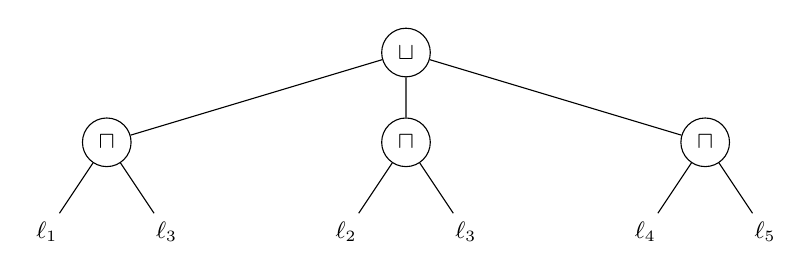
\begin{tikzpicture}[
  level distance=12mm,
  level 1/.style={sibling distance=40mm},
  level 2/.style={sibling distance=16mm},
  every node/.style={font=\small},
  op/.style={draw, circle, minimum size=6.5mm, inner sep=0.5mm},
  lit/.style={draw=none},
  scale=0.95, transform shape
]
\node[op] (root) {$\sqcup$}
  child { node[op] (cap1) {$\sqcap$}
    child { node[lit] {$\ell_1$} }
    child { node[lit] {$\ell_3$} }
  }
  child { node[op] (cap2) {$\sqcap$}
    child { node[lit] {$\ell_2$} }
    child { node[lit] {$\ell_3$} }
  }
  child { node[op] (cap3) {$\sqcap$}
    child { node[lit] {$\ell_4$} }
    child { node[lit] {$\ell_5$} }
  };
\end{tikzpicture}
\end{center}

\medskip
\noindent\textbf{\LUCO preservation.}
Comparing \LUCO relations before (as computed in Example~\ref{ex:AST}) and after normalization:
\begin{align*}
\LUCO_{\dnf(\phi)}(\ell_1,\ell_3) &= \sqcap \;=\; \LUCO_{\phi}(\ell_1,\ell_3),\\
\LUCO_{\dnf(\phi)}(\ell_2,\ell_3) &= \sqcap \;=\; \LUCO_{\phi}(\ell_2,\ell_3),\\
\LUCO_{\dnf(\phi)}(\ell_4,\ell_5) &= \sqcap \;=\; \LUCO_{\phi}(\ell_4,\ell_5),\\
\LUCO_{\dnf(\phi)}(\ell_1,\ell_2) &= \sqcup \;=\; \LUCO_{\phi}(\ell_1,\ell_2),\\
\LUCO_{\dnf(\phi)}(x,y) &= \sqcup \;=\; \LUCO_{\phi}(x,y)\quad
\text{for }x\in\{\ell_1,\ell_2,\ell_3\},\ y\in\{\ell_4,\ell_5\}.
\end{align*}
Thus the \LUCO \emph{label} is preserved by $\dnf$, even though the \LUCO node may move,
e.g.\ $\ell_1,\ell_2$ are separated by the root $\sqcup$ in $\dnf(\phi)$.
\end{example}

when a formula has a punctual conflict any of its
equivalent formula satisfying \LUCO and
\LAP have a punctional conflict.








% \begin{lemma}[Preservation of Boolean operator alternation under $\pnf$]\label{lem:alternation}
% For any formula $\phi \in \TDDLfm$ and any bound $k \in \mathbb{N}$, the transformation $\pnf(\phi,k)$ preserves the syntactic alternation of Boolean operators in $\phi$.  
% In particular, the relative structure of conjunctions and disjunctions among sub-formulas of $\phi$ is unchanged in $\pnf(\phi,k)$.
% \end{lemma}
% \begin{proof}
% By Definition~\ref{def:pnf}, we have $\pnf(\phi,k)$ is homomorphic for conjunction in disjunction operators:\\
% $\pnf(\phi_1 \sqcap \phi_2,k)=  \pnf(\phi_1,k) \sqcap\pnf(\phi_2,k)$ \nd $\pnf(\phi_1 \sqcup \phi_2,k)=  \pnf(\phi_1,k) \sqcup \pnf(\phi_2,k)$.
% \end{proof}



% \begin{lemma}[Ancestor preservation of literals under $\pnf$]\label{lem:pnf-no-new-literals}
% For any $k\in\mathbb{N}$, every formula $\phi\in\TDDLfm$, and $\tool{D} \in \{\tool{O}, \tool{F}\}$, every literal $\monadop{D}{\is}{a}$ that occurs as a literal in $\pnf(\phi,k)$ has an ancestor literal $\monadop{D}{\is'}{a}$ that occurs in $\phi$ with $\is  \subseteq \bigcup \is'$.
% In particular, if $\is=\{[t,t]\}$ is punctual, then $t\subin \is'$.
% \end{lemma}


% \begin{proof}
% We proceed by structural induction on $\phi$, case-splitting according to Definition~\ref{def:pnf}.

% \emph{Base case (literal).}  
% If $\phi=\ob{\is}{a}$, then $\pnf(\phi,k)$ is either
% \[
% \bigsqcup_{t\in\is}\ob{\{[t,t]\}}{a}
% \]
% when $\max(\is)\le k$,  
% or
% \[
% \left(\bigsqcup_{t\in\is\ominus[k+1,\infty]}\ob{\{[t,t]\}}{a}\right)
% \sqcup \ob{\is\cap[k+1,\infty]}{a}
% \]
% when $\max(\is)>k$.  
% In both cases, every produced literal has the same modality and action as the original, and its interval set is included in $\is$.  
% The case $\phi=\forb{\is}{a}$ is analogous, using conjunction and the operators $\is\ominus[k+1,\infty]$ and $\is\cap[k+1,\infty]$.
% \emph{Inductive step.}  
% If $\phi=\phi_1\sqcap \phi_2$, then $\pnf(\phi,k)=\pnf(\phi_1,k)\sqcap \pnf(\phi_2,k)$; any literal in $\pnf(\phi,k)$ occurs in one of the sub-formula, and the induction hypothesis gives its ancestor in $\phi_1$ or $\phi_2$.  
% The case $\phi=\phi_1\sqcup \phi_2$ is identical.
% Thus, every literal in $\pnf(\phi,k)$ has an ancestor in $\phi$ with the same $(D, a)$ and an interval set covering all its points.  
% \end{proof}

% \begin{lemma}[Witness punctualization into $\pnf$]\label{lem:witness-punct-pnf}
% Let $\phi\in\TDDLfm$, when $k=\textsc{MaxOPoint}(\phi)$, and let
% $\ell_i=\monadop{Di}{\is_{i}}{a_i}$ and
% $\ell_j=\monadop{Dj}{\is_{j}}{a_j}$
% be literals that \emph{occur in} $\phi$ under a common conjunctive context.
% If there exists $t\in\mathbb{N}$ with $t\subin \is_i$ and $t\subin \is_j$ and $t\le k$,
% then $\pnf(\phi,k)$ contains punctual descendants
% \[
% \ell_i^p=\monadop{Di}{\{[t,t]\}}{a_i}
% \quad\text{and}\quad
% \ell_j^p=\monadop{Dj}{\{[t,t]\}}{a_j},
% \]
% each occurring at the respective literal positions (i.e., as descendants of
% $\ell_i$ and $\ell_j$) within the same conjunctive context inherited from $\phi$.
% \end{lemma}

% \begin{proof}
% By Definition~\ref{def:pnf}, each literal is refined \emph{in place}:
% obligations produce a disjunction over all $t\in  \is\cap\{[0,k]\}$ of
% $\ob{\{[t,t]\}}{a}$; prohibitions produce a conjunction over those $t$ of
% $\forb{\{[t,t]\}}{a}$. Thus $t\le k$ and $t\subin\is_i$ (resp.$\is_j$)
% imply that $\ell_i^p$ (resp.\ $\ell_j^p$) appears among the descendants of
% $\ell_i$ (resp.\ $\ell_j$). By the operator-skeleton preservation lemma for
% $\pnf$ (Lemma~\ref{lem:alternation}), the enclosing conjunction from
% $\phi$ remains at the same place in $\pnf(\phi,k)$, so both punctual descendants
% occur within that same conjunctive context. 
% \end{proof}

% We move now to study the same properties for the $\dnf$ normalization.

% \begin{lemma}[Preservation of Boolean operator alternation and literal ancestor relation under $\dnf$]
% \label{lemma:dnf-alt-anc}
% Let $\phi \in \TDDLfm$. Then the transformation $\dnf(\phi)$ satisfies the following properties:
% \begin{enumerate}[(i)]
%     \item \textbf{Boolean alternation preservation:} The syntactic alternation between conjunction and disjunction in $\phi$ is preserved in $\dnf(\phi)$ in the sense that every Boolean connective in $\dnf(\phi)$ has the same relative position (conjunctive or disjunctive level) as in some equivalent sub-formula of $\phi$.
%     \item \textbf{ancestor Literal preservation:} For every literal $\ell$ occurring in $\dnf(\phi)$, there exists a literal $\ell'$ occurring in $\phi$ such that $\ell$ is syntactically identical to $\ell'$.
% \end{enumerate}
% \end{lemma}

% \begin{proof}
% \emph{(i) Alternation preservation:}  
% We prove by contradiction. Assume there exists a sub-formula in $\dnf(\phi)$ whose Boolean operator alternation pattern differs from any alternation pattern in $\phi$. The only transformation used to obtain $\dnf(\phi)$ from $\phi$ is repeated application of the distributivity equivalences in Lemma~\ref{lemma:operequiv}, which replace a sub-formula of the form \\
% $\phi_1 \sqcap (\phi_2 \sqcup \phi_3)$ by $(\phi_1 \sqcap \phi_2) \sqcup (\phi_1 \sqcap \phi_3)$, or symmetrically for disjunction over conjunction. These rewritings do not invert the order of $\sqcap$ and $\sqcup$ but only propagate one operator outward. Thus, any alternation pattern in $\dnf(\phi)$ is inherited from some subformula of $\phi$, contradicting the assumption. Hence alternation is preserved.

% \emph{(ii) Ancestor preservation:}  
% Again, we proceed by contradiction. Suppose there exists a literal $\ell$ in $\dnf(\phi)$ such that no identical literal occurs in $\phi$. The $\dnf$ transformation rewrites only via distributivity and associativity, which neither introduces new literals nor modifies their deontic operator or time interval. Therefore, every literal in $\dnf(\phi)$ must have appeared unchanged in $\phi$. This contradicts the assumption, hence ancestor preservation holds.
% \end{proof}


\begin{theorem}[Soundness and Completeness of Algorithm~\ref{fig:conflict-extraction}]
\label{lem:conflict-sound-complete}
Let $\phi$ be any formula in \TDDLfm, and let $k=\textsc{MaxOPoint}(\phi)$.
Then Algorithm~\ref{fig:conflict-extraction} is sound and complete for detecting punctual conflicts in $\phi$: the set $\mathcall{PC}(\phi)$ returned by the algorithm contains \emph{exactly} the punctual conflicts specified by $\phi$.
\end{theorem}

\begin{proof}
We prove both directions\\
\smallskip\noindent
(I) Soundness:\\
Take any $(\pt,\mathcall{C})\in\mathcall{PC}(\phi)$ and any $\hat\ell\sqcap \hat\ell'\in\mathcall{C}$.
By definition of conflicts, $\hat\ell,\hat\ell'$ are punctual literals at a common time $t$ that match one
of \textbf{(P-Deon-Conf)} or \textbf{(P-Ont-Conf)}, and they co-occur in a product term of
$\dnf(\pnf(\phi,k))$.
By Lemma~\ref{lem:pnf-ancestor} (downward) each has an ancestor $\ell,\ell'$ in $\phi$
with the same modality/action and covering $t$. By Lemma~\ref{lem:pnf-luco} followed by
Lemma~\ref{lem:dnf-luco}, we have: (i), the \LUCO relating the two positions is preserved across
$\pnf$ and $\dnf$, since they are present conjunctively in the product term, the \LUCO in $\phi$
is $\sqcap$. Hence $\ell\sqcap\ell'$ is a syntactically specified punctual pair in $\phi$,
of the same conflict type as $\hat\ell \sqcap \hat\ell'$ (types are syntactic and preserved).
Therefore, no product term forming a punctual conflict is introduced: every reported pair corresponds to one
already specified in $\phi$, and also its type(deontic vs ontic) is sound.

\smallskip\noindent
\emph{(II) Completeness.}  
\begin{enumerate}[(1)]
\item \textbf{All potential conflicts are exposed.}
Choose $k=\textsc{MaxOPoint}(\phi)$. Every time point relevant to \tool{O}/\tool{O} and
\tool{O}/\tool{F} conflicts is unfolded in $\pnf(\phi,k)$; prohibitions beyond $k$ cannot
yield punctual conflicts as there exists no conflict type involving two prohibitions. By Lemmas~\ref{lem:pnf-luco} and~\ref{lem:dnf-luco} (i), the \LUCO
for any literal pair is preserved through $\pnf$ and $\dnf$.

\item \textbf{All conflicts are localized and enumerated.}
If a conflict is specified in $\phi$ by a pair $\ell_i,\ell_j$ at some $t$ with
$\LUCO_\phi(\ell_i,\ell_j)=\sqcap$, then by Lemma~\ref{lem:witness-punct-pnf} there
exist punctual descendants at $t$ in $\pnf(\phi,k)$ under the same (conjunctive) \LUCO; by
Lemma~\ref{lem:dnf-luco} (ii) there is a product term of $\dnf(\pnf(\phi,k))$ containing both.
The algorithm checks \emph{every} pair in \emph{every} product term, ensuring that it catches them all.

\item \textbf{All conflict types are covered.}
By Lemma~\ref{lem:typeccomp}, punctual conflicts are exactly ontic or deontic.
The matching step of the algorithm recognizes precisely these patterns, so every possible punctual conflict is detected.
\end{enumerate}
By (I) and (II), we prove the correctness of the algorithm.
\end{proof}

After establishing the soundness and completeness of Algorithm~\ref{fig:conflict-extraction}, we analyze the cost of the full normalization chain that the algorithm relies on. The growth stems from two places: (i) \emph{punctual expansion} in $\pnf(\phi,k)$, which replaces each interval set by a boolean combination of punctual literals up to the bound $k$, and (ii) the \emph{cross-product} created when $\dnf$ distributes conjunctions over the disjunctions introduced by $\pnf$.

\begin{theorem}[Complexity of Full Normalization]\label{complexityofconf}
Let $\phi$ be a formula in \TDDLfm and let $k \in \mathbb{N}$ be a finite time bound. The transformation $\phi \to \dnf(\pnf(\phi,k))$ has worst-case space that is exponential in the average expansion factor of the interval sets in $\phi$ and the size of $\phi$.
\end{theorem}
\begin{proof}
We proceed in two stages, corresponding to the $\pnf$ and $\dnf$ transformations.

\textbf{Step 1: Punctual Normalization.}  
By Lemma~\ref{lem:pnf-size-expansion}, the size of the punctual normal form $\pnf(\phi,k)$ is bounded by a linear function of the original formula size and the average expansion factor of the interval sets:
\[
\pnf(\phi,k) \in \mathcall{O}\left( \expf_a(\phi) \cdot \size{\phi} \right).
\]
This step is therefore polynomial in $\size{\phi}$, assuming that $\expf_a(\phi)$ remains bounded.

\textbf{Step 2: Disjunctive Normalization.}  
By Lemma~\ref{lem:dnf}, every formula $\phi$ can be rewritten into an equivalent formula $\phi'$ in disjunctive normal form such that $\phi \dutyequiv \phi'$ and $\phi' := \bigsqcup_i \phi_i'$. However, the DNF transformation involves distributing conjunctions over disjunctions, which incurs an exponential increase in the number of product terms.

Each obligation literal $\ob{\is}{a}$ in $\pnf(\phi,k)$ generates a disjunction of size $\size{\is}$ (i.e., one punctual obligation per point), and each such disjunction contributes multiplicatively to the number of disjuncts in the DNF. Therefore, the number of product terms in $\dnf(\pnf(\phi,k))$ is at most exponential in the total number of punctual obligations introduced by $\pnf$, which is itself linear in $\expf_a(\phi) \cdot \size{\phi}$.

Thus, the total size of $\dnf(\pnf(\phi,k))$ is bounded by:
\[
\dnf(\pnf(\phi,k)) \in \mathcall{O}\left( 2^{\expf_a(\phi) \cdot \size{\phi}} \right),
\]
and so is the worst-case complexity of computing this transformation.
\end{proof}

We now prove the disjunctive modularity of our conflict detection algorithm.

\begin{lemma}[Conflict Extraction over Disjunctive Normal Form]
\label{lem:pc-dnf-union}
Let $\phi$ be a formula in \TDDLfm and let  $\phi':=\bigsqcup_{i=1}^n \phi_i'$ be the resulting formula from the disjunctive normalisation obtained according to Lemma~\ref{lem:dnf}.
Then the set of tuples product term, conflicts obtained for $\phi$ is the union of the set of tuples product term, conflicts in its disjuncts:
$$
\mathcall{PC}(\phi) = \bigcup_{i=1}^n \mathcall{PC}(\phi_i').
$$
\end{lemma}

\begin{lemma}[Conflict extraction over disjunctive normal form]
\label{lem:pc-dnf-union}
Let $\phi\in\TDDLfm$ and let $\phi':=\bigsqcup_{i=1}^n \phi_i'$ be the disjunctive normal form of $\phi$ obtained according to Lemma~\ref{lem:dnf}. Then the set of (product–term, conflict–set) tuples returned by the extractor satisfies
\[
\mathcall{PC}(\phi)\;=\;\bigcup_{i=1}^n \mathcall{PC}(\phi_i').
\]
\end{lemma}

\begin{proof}
Recall what the extractor $\mathcall{PC}(\,\cdot\,)$ does (Algorithm~\ref{fig:conflict-extraction}): given an input
$\phi$, it computes $k=\textsc{MaxOPoint}(\phi)$, forms $\dnf(\pnf(\phi,k))$, and then, for
\emph{each} product term $\pt$ occurring at the top level of that DNF, it computes the set
$\mathcall{C}(\pt)$ of punctual conflicts by inspecting all pairs of literals in $\pt$ and
matching the fixed patterns \textbf{P-Deon-Conf} and \textbf{P-Ont-Conf}. It returns the set
$\{(\pt,\mathcall{C}(\pt)) \mid \mathcall{C}(\pt)\neq\emptyset\}$.

Let $k=\textsc{MaxOPoint}(\phi)$, and write $\phi'=\dnf(\pnf(\phi,k))=\bigsqcup_{i=1}^n \phi_i'$,
where each $\phi_i'$ is (by construction of DNF) a single product term (a conjunction of punctual literals).

We prove the stated equality by double inclusion.

\smallskip\noindent
$\subseteq$: Take any $(\pt,\mathcall{C})\in\mathcall{PC}(\phi)$. By the algorithm, $\pt$ is one of
the top-level product terms of $\phi'$, hence $\pt=\phi_j'$ for some $j\in\{1,\dots,n\}$. When the
extractor is run on $\phi_j'$ alone, the preprocessing is inert:
$\pnf(\phi_j',k)=\phi_j'$ (already punctual) and $\dnf(\phi_j')=\phi_j'$ (already a conjunction).
Therefore, the same per-term analysis over pairs of literals in $\pt$ is performed, yielding the
same conflict set $\mathcall{C}$. Hence $(\pt,\mathcall{C})\in\mathcall{PC}(\phi_j')\subseteq
\bigcup_{i=1}^n \mathcall{PC}(\phi_i')$.

\smallskip\noindent
$\supseteq$: Take any $(\pt,\mathcall{C})\in\mathcall{PC}(\phi_i')$ for some $i$. Since
$\phi_i'$ is a top-level product term of $\phi'$, the run of the extractor on $\phi$ will visit
that very product term $\pt=\phi_i'$ and execute the identical per-term scan, thus producing the
same $\mathcall{C}$. Therefore $(\pt,\mathcall{C})\in\mathcall{PC}(\phi)$.

\smallskip
In both directions, we used the following facts (i) DNF puts each product term at the top level, and (ii) the
conflict check is \emph{local} to each product term (it never compares literals across distinct
disjuncts). Hence $\mathcall{PC}(\phi)=\bigcup_{i=1}^n \mathcall{PC}(\phi_i')$.
\end{proof}

% \vspace{1em}
% \textbf{Notes:}
% \begin{itemize}
%     \item \texttt{maxtime point} extracts the largest time $t$ in obligation literals of $\phi$.
%     \item \texttt{pnf} and \texttt{dnf} are normalization functions preserving semantic equivalence.
%     \item \texttt{matchesConflictPattern} checks if conjunction $c$ matches known punctual conflicts such as \textbf{P-Deon-Conf} or \textbf{P-Ont-Conf}.
% \end{itemize}







\begin{example}[Conflict extraction on $\UC_1'$ and $\UC_2'$]\label{punctual conflicts detect}
We apply Algorithm~\ref{fig:conflict-extraction} to each disjunct of the normalized formula. 
$$
\UC' := \UC_1' \sqcup \UC_2'.
$$

\textbf{Step 1: Maximal Time Point.}  
The maximal time point in the obligation literals is $k = 16$.

\textbf{Step 2: Punctual Normal Form.}  
We apply the $\pnf$ up to point 16 to each formula:
\[
\begin{aligned}
\pnf(\UC_1',16) &= 
\left( \bigsqcup_{\substack{t \subin\\ \{[9,16]\}}} 
\ob{\{[t,t]\}}{\delAtGate} \right)  \sqcap \left( 
\bigsqcap_{\substack{t \subin\\ \{[2,4],[8,16]\}}} 
\forb{\{[t,t]\}}{\delAtGate} \sqcap 
\forb{\{[17,24]\}}{\delAtGate} \right)\\
&\quad \sqcap \left( \bigsqcap_{\substack{t \subin\\ \{[10,14]\}}} 
\forb{\{[t,t]\}}{\delAtPark} \right). \\
\pnf(\UC_2',16) &= 
\left( \bigsqcup_{\substack{t \subin\\ \{[9,16]\}}} 
\ob{\{[t,t]\}}{\delAtPark} \right) \sqcap \left( \bigsqcap_{\substack{t \subin\\ \{[10,14]\}}} 
\forb{\{[t,t]\}}{\delAtPark} \right) \\
& \quad \sqcap \left( 
\bigsqcap_{\substack{t \subin\\ \{[2,4],[8,16]\}}} 
\forb{\{[t,t]\}}{\delAtGate} \sqcap 
\forb{\{[17,24]\}}{\delAtGate} \right).
\end{aligned}
\]

\textbf{Step 3: Disjunctive Normal Form.}  
Distribute conjunction over disjunction to obtain \dnf. Each disjunct is formed by fixing one 
$t \subin \{[9,16]\}$ in the obligation disjunction.
\[\begin{array}{c}

				\dnf(\pnf(\UC_1',16))\\
				= \\
				\mathop{\bigsqcup}\limits_{\substack{t \subin\\ \{[9,16]\}}}
\left(
  \ob{\{[t,t]\}}{\delAtGate}
  \sqcap
  \mathop{\bigsqcap}\limits_{\substack{t' \subin\\ \{[10,14]\}}}
    \forb{\{[t',t']\}}{\delAtPark}
  \sqcap
  \mathop{\bigsqcap}\limits_{\substack{t'' \subin\\ \{[2,4],[8,16]\}}}
    \forb{\{[t'',t'']\}}{\delAtGate}
  \sqcap
  \forb{\{[17,24]\}}{\delAtGate}
\right)
\\
			\end{array}\]

and 
\[\begin{array}{c}

				\dnf(\pnf(\UC_2',16))\\
				= \\
				\mathop{\bigsqcup}\limits_{\substack{t \subin\\ \{[9,16]\}}}
\left(
  \ob{\{[t,t]\}}{\delAtPark}
  \sqcap
  \mathop{\bigsqcap}\limits_{\substack{t' \subin\\ \{[10,14]\}}}
    \forb{\{[t',t']\}}{\delAtPark}
  \sqcap
  \mathop{\bigsqcap}\limits_{\substack{t'' \subin\\ \{[2,4],[8,16]\}}}
    \forb{\{[t'',t'']\}}{\delAtGate}
  \sqcap
  \forb{\{[17,24]\}}{\delAtGate}
\right)
\\
			\end{array}\]



\textbf{Step 4: Conflict Detection.}  
The last step, which involves pattern matching conflicts, exhibits punctual conflicts $\UC_1'$. The punctual conflicts are of type deontic and are on product terms formed by the obligations on time points $10,11,12,13,\nd 14$ :
\[
\big\{
\ob{\{[t,t]\}}{\delAtGate} \sqcap \forb{\{[t,t]\}}{\delAtPark} \ \big| \ 
t \subin \{[10,14]\}
\big\}.\]

For $\UC_2'$, the algorithm detects deontic punctual conflicts in all product terms:
\[\
\big\{
\ob{\{[t,t]\}}{\delAtPark} \sqcap \forb{\{[t,t]\}}{\delAtPark} \ \big| \ 
t \subin \{[9,16]\}
\big\}.
\]
\end{example}









The example showcased two possible successful detections of punctual conflicts in two of the sub-formulas of our use case, namely $\UC_1' \nd \UC_2'$. Where $\UC_1'$ contained some conflicting product terms and $\UC_2'$ had punctual conflicts in all its product terms. We have also studied the satisfiability of the same sub-formulas in Example~\ref{satsolver}, and we have obtained that $\DC_1'$ is satisfiable and $\DC_2'$ is unsatisfiable.


We introduce the notion of \emph{conflict density} as a measure to quantify the prevalence of conflicts within normative specifications. High conflict density signals practical difficulty: it shrinks the set of specified feasible behaviors available to an agent, complicates compliance checking and planning, and blurs the specification's comprehensibility.  By formally capturing conflict density in  Def.~\ref{def:Conflict density-measure}, we provide a practical metric to guide the systematic refinement of normative specifications, supporting normative system designers in identifying and addressing overly restrictive or contradictory constraints.

\begin{definition}[Conflict Density]\label{def:Conflict density-measure}
Let $\phi$ be a formula from \TDDLfm and $k= \textsc{MaxOPoint}(\phi)$.  
We define the \defn{conflict density} for the formula $\phi$, written  $\cd(\phi)$, as the ration between the conflicting product terms and the the total number of product terms in $\dnf(\pnf(\phi,k))$, formally:
$$
\cd(\phi) := \frac{\size{\mathcall{PC}(\phi)}}{\Xi(\phi)} \quad.
$$
Where:
\begin{itemize}
    \item $\size{\mathcall{PC}(\phi)}$ is the cardinality of the set of pairs returned by  Algorithm~\ref{fig:conflict-extraction} on $\phi$, and
    \item $\Xi(\phi)$ is \defn{the number of product terms} in $\dnf(\pnf(\phi,k))$.
\end{itemize}
\end{definition}
The conflict density $\cd(\phi)$ captures the proportion of conflicting punctual obligations  that are involved in conflicts, providing an indicator of how overloaded the normative specification is, that is, the fraction of time points where an obligation is prescribed but cannot actually be fulfilled. When $\cd(\phi)=0$ we say that $\phi$ is \defn{conflict free}, and $\phi$ is said to be \defn{fully conflicting} when $\cd(\phi)=1$.

\begin{example}[Conflict density measure computation]
We now compute the conflict density measure $\cd(\phi)$ based on the analysis done for Example~\ref{ex:easy}.

From Table~\ref{table:conflict-analysis}, we know that:
\begin{itemize}
    \item The number of product terms in $\dnf(\pnf(\phi,2))$ is $\Xi(\phi) = 4$,
    \item The number of product terms containing at least one punctual conflict  is $\size{\mathcall{PC}(\phi)} = 3$.
\end{itemize}

Hence, by Definition~\ref{def:Conflict density-measure}, we compute the conflict density measure as:
$$
\cd(\phi) = \frac{3}{4} = 0.75.
$$
This conflict density value indicates a high level of conflict density, as 75\% of the product terms are involved in conflicts, either deontic or ontic. In practice, such a high conflict density may suggest  overloaded normative constraints in the normative specification.
\end{example}


\begin{example}[Computing conflict density measure for $\UC_1'$ and $\UC_2'$]\label{ex:Conflict density-UC1-UC2}
Building on Example~\ref{punctual conflicts detect}, we compute the Conflict density measure for the disjuncts $\UC_1'$ and $\UC_2'$ individually.

\textbf{Step 1: Conflict Count.}  
From the conflict detection phase, we have clauses containing exactly one conflict per clause:
\[
\mathcall{PC}(\UC_1') = 
\big\{
\ob{\{[t,t]\}}{\delAtGate} \sqcap \forb{\{[t,t]\}}{\delAtGate} \sqcap \forb{\{[2,4],[8,24]\}}{\delAtPark} \ \big| \ t \subin \{[10,14]\}
\big\}, \quad \text{so } \size{\mathcall{PC}(\UC_1')} = 5.
\]

\[
\mathcall{PC}(\UC_2') = 
\big\{
\ob{\{[t,t]\}}{\delAtPark} \sqcap \forb{\{[t,t]\}}{\delAtPark} \ \big| \ t \subin \{[9,16]\}
\big\}, \quad \text{so } \size{\mathcall{PC}(\UC_2')} = 8.
\]

\textbf{Step 2: Obligation Count.}  
From the Punctual Normal Form \pnf up to 16 we know:
\[
\UC_1' \text{ generates } 8 \text{ punctual obligations on } \delAtGate \quad (t \subin \{[9,16]\}),
\]
\[
\UC_2' \text{ generates } 8 \text{ punctual obligations on } \delAtPark \quad (t \subin \{[9,16]\}).
\]

\textbf{Step 3: Conflict density Measures.}
\[
\cd(\UC_1') = \frac{\size{\mathcall{PC}(\UC_1')}}{\Xi(\UC_1')} = \frac{5}{8} = 0.625,
\]
\[
\cd(\UC_2') = \frac{\size{\mathcall{PC}(\UC_2')}}{\Xi(\UC_2')} = \frac{8}{8} = 1.
\]


$\UC_2'$ has conflict density of 1, with every punctual obligation point involved in a conflict.  
$\UC_1'$ has a conflict density less than 1, with conflicts at five of the eight obligation points.

We move now to do it for the overall use case we have, following Lemma~\ref{lem:pc-dnf-union}: \[
\mathcall{PC}(\UC) = \mathcall{PC}(\UC_1') \cup \mathcall{PC}(\UC_2').
\]

with:
\[
\size{\mathcall{PC}(\UC_1')} = 5 \quad \text{and} \quad \size{\mathcall{PC}(\UC_2')} = 8.
\]
So:
\[
\size{\mathcall{PC}(\UC)} = 13.
\]

\textbf{Obligation count.}  
From the punctual normal form construction:
\[
\UC_1' \text{ and } \UC_2' \text{ each produce } 8 \text{ punctual obligations (1 per } t \subin \{[9,16]\}).
\]
Thus:
\[
\Xi(\UC) = 16.
\]

\textbf{Conflict density measure.}  
Applying the definition:
\[
\cd(\UC) = \frac{\size{\mathcall{PC}(\UC)}}{\Xi(\UC)} = \frac{13}{16} \approx 0.8125.
\]
This indicates that approximately 81\% of punctual obligation points in $\UC$ are involved in conflicts and thus cannot be used to comply with the normative system.
\end{example}

We proceed to study the relationship between the unsatisfiability of a formula and its conflict density.
\begin{lemma}[Fully conflicting means Unsatisfiable]
\label{lem:full-Conflict density-unsat}
Let $\phi$ be a formula in \TDDLfm. Then $\phi$ is fully conflicting, i.e., $\cd(\phi) = 1$, if and only if $\phi$ is unsatisfiable.
\end{lemma}


\begin{proof}
($\Rightarrow$) Assume $\cd(\phi) = 1$.  
By Definition~\ref{def:Conflict density-measure}, we have:
$$
\frac{\size{\mathcall{PC}(\phi)}}{\Xi(\phi)} = 1.
$$
This implies that every punctual obligation literal generated by $\pnf(\phi,k)$ participates in a punctual conflict. In the \dnf expansion of $\pnf(\phi)$, each product term includes at least one such obligation, and by definition of punctual conflict, this yields an unsatisfiable conjunction by conjunction extension. Since all product terms are unsatisfiable, their disjunction is unsatisfiable. Hence, $\phi$ is unsatisfiable.

($\Leftarrow$) Now assume $\phi$ is unsatisfiable.  
By Lemma~\ref{lem:pc-dnf-union}, the set of punctual conflicts $\mathcall{PC}(\phi)$ is the union of the punctual conflicts found in each \dnf disjunct. If $\phi$ is unsatisfiable, there exists no word satisfying the formula. Then every product term in $\dnf(\pnf(\phi, k))$ must also be unsatisfiable, so each contains a punctual conflict. Moreover, since an unsatisfiable formula must have all its obligation points involved in conflict (otherwise at least one satisfying assignment would exist for a disjunct), it follows that:
$$
\size{\mathcall{PC}(\phi)} = \Xi(\phi),
$$
and hence $\cd(\phi) = 1$.

Therefore, $\phi$ is fully conflicting if and only if it is unsatisfiable.
\end{proof}


\begin{theorem}[Conflict free pruning for Partially conflicting Formulas]
\label{thm:pruning-partial-Conflict density}
Let $\phi\in\TDDLfm$ with $\cd(\phi)\neq 1$ (i.e., $\phi$ is not fully conflicting). 
Then there exists a formula $\phi'$ such that
\[
\phi \equiv \phi' \quad\text{and}\quad \cd(\phi')=0.
\]
\end{theorem}

\begin{proof}[Proof (by constructive pruning via Algorithm~\ref{fig:conflict-extraction})]
Let $k=\textsc{MaxOPoint}(\phi)$ and build 
\[
\phi_{\text{dpnf}} \ :=\ \dnf(\pnf(\phi,k)) \ =\ \bigsqcup_{i=1}^{n}\pt_i,
\]
where each $\pt_i$ is a product term (conjunction of punctual literals).

Run Algorithm~\ref{fig:conflict-extraction} on $\phi$ and obtain
\[
\mathcall{PC}(\phi)\ =\ \{\,(\pt_i,\mathcall{C}_{\pt_i})\ :\ 1\le i\le n,\ \mathcall{C}_{\pt_i}\neq\emptyset\,\}.
\]
By definition of $\cd$ (Definition~\ref{def:Conflict density-measure}), $\cd(\phi)\neq 1$ implies that \emph{not all} product terms are conflicting, i.e., the index set formed by non-conflicting product terms
$
I\ :=\ \{\, i\in\{1,\dots,n\} \mid \mathcall{C}_{\pt_i}=\emptyset \,\}$ is nonempty.

Define the pruned disjunction
\[
\phi' \ :=\ \bigsqcup_{i\in I}\ \pt_i.
\]

\emph{Equivalence.}
By Lemma~\ref{lem:dpnf-semantics}, $\phi\equiv \phi_{\text{dpnf}}$.
For every $j\notin I$, Algorithm~\ref{fig:conflict-extraction} returned a nonempty conflict set $\mathcall{C}_{\pt_j}\neq\emptyset$, meaning $\pt_j$ contains a punctual conflict. By the definition of punctual conflict and closure under conjunction, each such $\pt_j$ is unsatisfiable. Hence
\[
\phi_{\text{dpnf}}\ \equiv\ \Big(\bigsqcup_{i\in I}\pt_i\Big)\ \sqcup\ \Big(\bigsqcup_{j\notin I}\underbrace{\pt_j}_{\bot}\Big)\ \equiv\ \bigsqcup_{i\in I}\pt_i\ =\ \phi'.
\]
Therefore $\phi\equiv \phi'$.

\emph{Zero conflict density.}
By construction, every disjunct $\pt_i$ retained in $\phi'$ satisfies $\mathcall{C}_{\pt_i}=\emptyset$. Thus $\mathcall{PC}(\phi')=\emptyset$ and, by Def.~\ref{def:Conflict density-measure}, $\cd(\phi')=0$.

This completes the constructive proof: $\phi'$ is obtained by (i) computing $\pnf$ and $\dnf$, (ii) calling Algorithm~\ref{fig:conflict-extraction} to mark conflicting product terms, and (iii) disjoining only the conflict-free ones.
\end{proof}

Having established that Algorithm~\ref{fig:conflict-extraction} is sound and complete for detecting punctual conflicts, we now turn to the question of how to refine a formula by \emph{eliminating} such conflicts. The idea is to discard any product term in the disjunctive punctual normal form that contains a conflict, thereby retaining only those disjuncts that remain consistent. This yields a conflict-free rewriting of the input formula, which we denote by $\Namb(\phi)$. By construction and by Theorem~\ref{lem:conflict-sound-complete}, every conflict identified and removed in this process corresponds to a genuine conflict specified by $\phi$, ensuring the soundness of the refinement. Formally, a variant of this algorithm would consist of: if every product term of $\dnf(\pnf(\phi,k))$ contains a punctual conflict, then no refinement is possible and the procedure returns \textbf{False}. Otherwise, $\Namb(\phi)$ is defined as the disjunction of all conflict-free product terms. The construction is given in Algorithm~\ref{alg:conflict-free-rewriting}.




\begin{minipage}{0.95\textwidth}
    \center{
\begin{algorithm}[H]
\caption{Procedure \textsc{Conflict-Free Rewriting} \Namb}
\label{alg:conflict-free-rewriting}
\KwIn{A formula $\phi \in \TDDLfm$}
\KwOut{\textbf{False} if every product term contains a punctual conflict; else a conflict-free refined formula $\Namb(\phi)$}

\BlankLine
$k \gets \textsc{MaxOPoint}(\phi)$ \tcp*{Largest obligation time point in $\phi$}

$\phi_{\mathrm{pnf}} \gets \pnf(\phi, k)$ \tcp*{Punctual normal form up to $k$}

$\phi_{\mathrm{dnf}} \gets \dnf(\phi_{\mathrm{pnf}})$ \tcp*{Convert to disjunctive normal form}

$\CF(\phi) \gets \emptyset$ \tcp*{Will collect non-conflicting product terms}

\ForEach{product term $\pt$ in $\phi_{\mathrm{dnf}}$}{
  $\textit{hasConflict} \gets \textbf{false}$\;
  \ForEach{pair of literals $(\ell_1,\ell_2)$ in $\pt$}{
    \If{$(\ell_1,\ell_2)$ matches \textbf{P-Deon-Conf} or \textbf{P-Ont-Conf}}{
      $\textit{hasConflict} \gets \textbf{true}$\;
      \textbf{break} \tcp*{No need to inspect more pairs in this $\pt$}
    }
  }
  \If{\textbf{not} $\textit{hasConflict}$}{
    $\CF(\phi) \gets \CF(\phi) \cup \{\pt\}$ \tcp*{Keep $\pt$: it is conflict-free}
  }
}

\If{$\CF(\phi)=\emptyset$}{
  \Return \textbf{False} \tcp*{All disjuncts have conflicts}
}
$\Namb(\phi) \gets \displaystyle\bigsqcup_{\pt \in \CF(\phi)} \pt$ \tcp*{Rebuild from conflict-free terms}
\Return $\Namb(\phi)$

\end{algorithm}}
\end{minipage}

\begin{remark}
    An optimized variant of Algorithm~\ref{alg:conflict-free-rewriting} can be obtained by incorporating an early satisfiability check. Before initiating the normalization and conflict-removal procedure, we first test whether the input formula $\phi$ is unsatisfiable, for instance using \textsc{checksat}$(\phi)$. If the result is negative, the procedure immediately returns \textbf{False}, since no conflict-free refinement can exist. This optimization avoids the potentially expensive construction of the punctual and disjunctive normal forms in cases where the formula is already inconsistent at the semantic level.
\end{remark}


The constructive pruning proof above does more than guarantee existence: it \emph{computes} the conflict-free disjuncts explicitly. Each conflict-free product term can be read as an executable policy clause. The next remark makes this operational connection precise.

\begin{remark}[Relation to planning]
Our pruning view is closely related to model enumeration (All-SAT), a standard task in SAT/SMT and Constraint Satisfaction Problem (CSP) as in ~\cite{valiant1979complexity,gomes2008model,creignou2011enumerating}. After removing all conflicting product terms from the \dpnf, what remains is a precisely delimited set of conforming, norm-following paths that a planner can safely execute. Each remaining disjunct specifies a consistent set of time-stamped obligations and prohibitions, i.e., a feasible and normatively compliant policy fragment.

A practical strategy is: (i) within a chosen product term, merge all prohibitions on the same action into a single prohibition interval set so that only punctual obligations remain as clear action points; and (ii) execute exactly those obligations at their designated time points while abstaining from all prohibited actions. This reduces planning to selecting one conflict-free clause, reading off its obligation timestamps, and committing to those actions. The choice is also explainable, e.g., “We selected product term~2, so we act at times $\{t_1,t_2,\dots\}$ and avoid all other actions by construction.”
\end{remark}

\noindent Having framed conflict elimination as a generator of clear, compliant planning options, we now turn to an orthogonal concern: the \emph{conciseness} of the resulting representation. Although our analysis detects and removes conflicts, the intermediate normalizations (\pnf and \dnf) can dramatically increase syntactic size. In the next subsection, we discuss this blow-up.


\subsection{Induced Verbosity from Eliminating Punctual Conflicts}\label{induced verbosity}

Eliminating punctual ontic conflicts yields conflict free formulas, but it can substantially increase syntactic size. The source of this blow-up is combinatorial: to respect the “at most one action per time point” assumption, one may enumerate only those product terms whose punctual obligations are scheduled at pairwise distinct times.


\begin{example}
\[
\phi \;:=\; \ob{\{[0,3]\}}{\mathsf{a}} \ \sqcap\  \ob{\{[0,3]\}}{\mathsf{b}} \ \sqcap\  \ob{\{[0,3]\}}{\mathsf{c}}.
\]
All three obligation literals share the same interval set and are conjoined, so at each $t\in\{0,1,2,3\}$ the pairwise $\tool{O}$–$\tool{O}$ combinations (e.g., $\ob{\{[t,t]\}}{\mathsf{a}}\sqcap\ob{\{[t,t]\}}{\mathsf{b}}$) yield punctual ontic conflicts.

Table~\ref{table:ontic-triple-conflict} shows the transformation pipeline: \pnf, \dnf, conflict extraction, and the construction of a conflict free rewriting $\Namb(\phi)$ that prunes all conflicting product terms. As the last row indicates, $\Namb(\phi)$ is about $20\times$ larger than the original $\phi$ under our size metric.

Intuitively, $\dnf(\pnf(\phi,3))$ enumerates all $4^3$ assignments of times to $(\mathsf{a},\mathsf{b},\mathsf{c})$. To avoid ontic conflicts, we must keep only those assignments where the three times are \emph{pairwise distinct}, i.e., $4\cdot3\cdot2=24$ product terms. This necessary filtering still yields a sizeable disjunction.

\begin{table}[h]
\centering
\renewcommand{\arraystretch}{1.5}
\begin{tabular}{|l|p{8cm}|c|}
\hline
\textbf{Step} & \textbf{Expression} & \textbf{Size} \\
\hline
$\phi$ 
& 
$\ob{\{[0,3]\}}{\mathsf{a}} \ \sqcap\  \ob{\{[0,3]\}}{\mathsf{b}} \ \sqcap\  \ob{\{[0,3]\}}{\mathsf{c}}$
& 18 \\
\hline
$\pnf(\phi,3)$ 
& 
$\Big( \bigsqcup_{i=0}^{3} \ob{\{[i,i]\}}{\mathsf{a}} \Big)
\ \sqcap\
\Big( \bigsqcup_{i=0}^{3} \ob{\{[i,i]\}}{\mathsf{b}} \Big)
\ \sqcap\
\Big( \bigsqcup_{i=0}^{3} \ob{\{[i,i]\}}{\mathsf{c}} \Big)$
& 59 \\
\hline
$\dnf(\pnf(\phi,3))$ 
& 
$\displaystyle
\bigsqcup_{\substack{0 \leq i,j,k \leq 3}} 
\Big( \ob{\{[i,i]\}}{\mathsf{a}} \ \sqcap\  \ob{\{[j,j]\}}{\mathsf{b}} \ \sqcap\  \ob{\{[k,k]\}}{\mathsf{c}} \Big)
$
& 959 \\
\hline
Punctual conflicts 
& 
$\displaystyle
\big\{
\ob{\{[t,t]\}}{\mathsf{a}} \sqcap \ob{\{[t,t]\}}{\mathsf{b}},\
\ob{\{[t,t]\}}{\mathsf{a}} \sqcap \ob{\{[t,t]\}}{\mathsf{c}},$
& -- \\
in $\mathcall{PC}(\phi)$ &$
\ob{\{[t,t]\}}{\mathsf{b}} \sqcap \ob{\{[t,t]\}}{\mathsf{c}}
\ \big|\ t\in\{0,1,2,3\}
\big\}
$ &
\\
\hline
$\Namb(\phi)$
& 
$\displaystyle
\bigsqcup_{\substack{i,j,k \in \{0,1,2,3\}\\ \text{pairwise distinct}}}
\Big( \ob{\{[i,i]\}}{\mathsf{a}} \ \sqcap\  \ob{\{[j,j]\}}{\mathsf{b}} \ \sqcap\  \ob{\{[k,k]\}}{\mathsf{c}} \Big)
$
& 359 \\
\hline
$\displaystyle \frac{\size{\Namb(\phi)}}{\size{\phi}}$ 
& 
Conflict elimination blow-up factor 
& $\approx 20$ \\
\hline
\end{tabular}
\caption{Conflict elimination size comparison for $\phi := \ob{\{[0,3]\}}{\mathsf{a}} \sqcap \ob{\{[0,3]\}}{\mathsf{b}} \sqcap \ob{\{[0,3]\}}{\mathsf{c}}$.}
\label{table:ontic-triple-conflict}
\end{table}
\end{example}

While the worst case can be large, a conflict free rewrting of a formula often admits a more concise equivalent by \emph{merging} punctual literals on the same action. In particular, disjunctions of punctual obligations on the same action can be compressed by \textbf{ObDis}, and conjunctions of punctual prohibitions can be compressed by \textbf{FConj}.

\begin{example}
Consider
\[
\UC_2' \;:=\; \ob{\{[9,16]\}}{\delAtPark} \ \sqcap\  \forb{\{[10,14]\}}{\delAtPark} \ \sqcap\  \forb{\{[2,4],[8,24]\}}{\delAtGate}.
\]
The conflict free rewriting $\Namb(\UC_2')$ prunes all conflicting product terms, leaving exactly the non-conflicting obligation times $t\in\{9,15,16\}$. A literal (still verbose) form is:
\begin{table}[h] \centering \renewcommand{\arraystretch}{1.5} \begin{tabular}{|l|p{10.5cm}|c|} \hline \textbf{Formula} & \textbf{Expression} & \textbf{Size} \\ \hline $\UC_2'$ & $\ob{\{[9,16]\}}{\delAtPark} \sqcap \forb{\{[10,14]\}}{\delAtPark} \sqcap \forb{\{[2,4], [8,24]\}}{\delAtGate}$ & 16 \\ \hline
     $\Namb(\UC_2')$ & $ \left(
        \ob{\{[9,9]\}}{\delAtPark}
        \sqcup
        \ob{\{[15,15]\}}{\delAtPark}
        \sqcup
        \ob{\{[16,16]\}}{\delAtPark}
      \right)
      \sqcap
      \mathop{\bigsqcap}\limits_{t \in [10,14]}
      \forb{\{[t,t]\}}{\delAtPark}
      \sqcap
        \forb{\{[2,4],[8,24]\}}{a} $ & 94 \\ 
     \hline $\UC_2''$ & $\ob{\{[9,9], [15,16]\}}{\delAtPark} \sqcap \forb{\{[10,14]\}}{\delAtPark} \sqcap \forb{\{[2,4], [8,24]\}}{\delAtGate}$ & 18 \\ \hline \end{tabular} \caption{Refactoring a verbose conflict free rewriting $\Namb(\UC_2')$ into a more concise equivalent $\UC_2''$.} \label{table:refactoring-uc2} \end{table}
Here $\UC_2''$ compresses the three surviving punctual obligations on \delAtPark\ into a single obligation over $\{[9,9],[15,16]\}$, while prohibitions on \delAtGate\ are merged back into their original interval sets.
\end{example}

These examples motivate \emph{controlled} conflict density management: when readability/size matters, designers can (i) keep compact high-level formulas that \emph{implicitly} contain ontic conflicts and resolve them later during planning, or (ii) eliminate conflicts upfront and then refactor the resulting \dpnf\ with merging rules (\textbf{ObDis}, \textbf{FConj}) to restore conciseness. In the next section, we present a generalized conflict rule over punctual literals that unifies deontic and ontic cases and supports concise rewritings without fully enumerating the \dpnf.

\subsection{Generalized Conflict Rules and Conflict Calculus}\label{subsec:calculus}
The previous section demonstrated that eliminating punctual conflicts may lead to significant increases in formula size. While some verbose conflict free rewriting formulas can be refactored into more concise forms, this is not always possible without losing semantic precision. In this section, we generalize the conflict scenarios observed earlier and formalize them as inference rules. These rules allow the user to explore the formula and choose which conflicts to remove.


We define in Table~\ref{syncnotation} syntactic notations build upon the extensional semantics from our logical framework to express rules for our deductive conflict analysis system. It introduces derivations such as entailment ($\vdash$) and equivalence ($\equiv$). Notice that if $\phi \vdash \phi'$ and $\phi' \vdash \phi$ then $\phi \equiv \phi'$ and $\phi' \equiv \phi$:
 \begin{itemize}
 \item We denote by $\phi \dutymodel \bot$ that the formula $\phi$ is inconsistent in our reasoning, i.e., it is unsatisfiable, so $\dutyclass{\phi} = \emptyset$. 
\item We denote by $\dutymodel \phi$ that the formula $\phi$ is valid in our proof system, we map it to its satisfiability by any possible \timedword, i.e., $\dutyclass{\phi} = 2^\domtr$.    
\item We denote by $\phi\dutymodel \phi'$ that formula $\phi$ entails $\phi'$, which holds when $\dutyclass{\phi} \subseteq \dutyclass{\phi'}$.   
\item Equivalence is written as $\phi \dutyequiv \phi$, which holds when $\dutyclass{\phi} = \dutyclass{\phi'}$. 
\end{itemize}

\begin{table}[h]
    \centering
    \begin{tabular}{|c|c|c|}
      \hline
      \emph{Notation} & \emph{Signification} & \emph{Semantic mapping} \\ \hline
      $\phi \vdash \bot$ 
        & $\phi$ is inconsistent 
        & $\dutyclass{\phi} = \emptyset$ \\ \hline
      $\vdash \phi$ 
        & $\phi$ is valid 
        & $\dutyclass{\phi} = 2^{\domtr}$ \\ \hline
      $\phi \vdash \phi'$ 
        & $\phi$ entails $\phi'$ 
        & $\dutyclass{\phi} \subseteq \dutyclass{\phi'}$ \\ \hline
      $\phi \equiv \phi'$ 
        & $\phi$ is equivalent to $\phi'$ 
        & $\dutyclass{\phi} = \dutyclass{\phi'}$ \\ \hline
    \end{tabular}
    \caption{Syntactic notations and their semantic mapping}
    \label{syncnotation}
  \end{table}
		


\subsubsection{Generalized conflicts}
We generalize from punctual conflicts to: \emph{deontic conflicts} and \emph{ontic conflicts}. The following two lemmas define the conditions under which these conflicts arise and how they can be either detected as inconsistencies or rewritten into equivalent but non-conflicting forms.


\begin{lemma}[Deontic Conflicts]\label{Gdeontic- conflict}
Let $\is$ and $\is'$ be interval sets, and let $\acta$ be an action. Then the following conflicts hold between an obligation and a prohibition:
\begin{enumerate}[(i)]
    \item If $\is \subseteq \is'$, then:
    $$
    \ob{\is}{a} \sqcap \forb{\is'}{a} \vdash \bot
    $$
    
    \item  If $\is \cap \is' \neq \emptyset$ and $\is \not\subseteq \is'$, then:
    $$
    \ob{\is}{a} \sqcap \forb{\is'}{a} \dutyequiv \ob{\is \ominus \is'}{a} \sqcap \forb{\is'}{a}
    $$
    where $\is \ominus \is'$ denotes the set difference between $\is$ and $\is'$.
\end{enumerate}

\end{lemma}
The first point $(i)$ from the lemma captures a case of full contradiction between an obligation and a prohibition over the same action and time frame; we will refer to it as \defn{full deontic conflict}. It reflects a semantic inconsistency; no behavior can satisfy both. The second point provides a rewriting strategy when the formula has conflicting points but is still satisfiable. We refer to this case as \defn{partial deontic conflict}.


\begin{proof}
    \leavevmode
    
    \textbf{(i) T-DeoConf:}  
    Let $\is \subseteq \is'$. Then every time point at which the action $\acta$ is required is also explicitly forbidden $t \subin \is \text{ then }  t \subin \is' $. Since punctual obligations and prohibitions are strict—meaning $\ob{\{[t,t]\}}{a}$ requires $\acta$ to occur exactly at $t$, and $\forb{\{[t,t]\}}{a}$ forbids it at $t$—this leads to an unsatisfiable situation at each $t \in \is$. There is no model in which $\acta$ can be both required and forbidden simultaneously. Thus, the conjunction of the two literals reduces to:
    $$
    \ob{\is}{a} \sqcap \forb{\is'}{a} \equiv \bigsqcup_{t\subin \is}\big(\ob{\{[t,t]\}}{a} \sqcap \forb{\{[t,t]\}}{a} \sqcap \forb{\{\is' \ominus \{[t,t]\}}{a} \big).
    $$ 
    
    \textbf{(ii) P-DeoConf:}  
    Assume $\is \cap \is' \neq \emptyset$ and $\is \not\subseteq \is'$. 
    In this case, the obligation and prohibition partially overlap in time, generating punctual conflicts at every $t \in \is \cap \is'$. 
    These conflicts render the specification unsatisfiable at the overlapping points. 
    However, outside this conflict zone, that is, for $t \in \is \setminus \is'$, the obligation remains uncontested and can therefore be preserved.
    
    
    In such cases, we can resolve the partial conflict by dropping the punctual obligations that fall within $\is \cap \is'$ (which are semantically void due to contradiction), and keeping only those that fall outside the prohibition interval. This yields a semantically equivalent formula:
    $$
    \ob{\is}{a} \sqcap \forb{\is'}{a} 
    \dutyequiv 
    \ob{\is \ominus \is'}{a} \sqcap \forb{\is'}{a}.
    $$
    This rewriting ensures that no punctual deontic conflict remains, while preserving all non-conflicting normative semantic equivalence.
    \end{proof}
    
    \begin{lemma}[Full Ontic Conflict]
    \label{lemma:ontic-conflict}
    Let $\is$ be a finite interval set with $\size{\is} < \infty$ and $\{a_1, \dots, a_n\}$ be a set of distinct actions such that:
    $$
    \size{\is} <_\infty \size{\{a_1, \dots, a_n\}},
    $$
    then the following holds:
    $$
    \bigsqcap_{i=1}^n \ob{\is}{a_i} \dutymodel \bot.
    $$
    \end{lemma}
    This lemma captures a generalization of punctual deontic conflicts. It suggests only the case of \defn{full ontic conflict} when there are too many actions to be performed within an insufficient time window. Unlike the case of deontic conflicts, we do not suggest any rewriting for partial cases due to their verbosity, as discussed in the previous section.
    
    \begin{proof}
    Let $\is$ be a finite interval set such that $\size{\is} = m$, and suppose $\{a_1, \dots, a_n\}$ is a set of distinct actions with $n > m$. Each literal $\ob{\is}{a_i}$ expands under $\pnf$ into:
    $$
    \ob{\is}{a_i} \dutyequiv \bigsqcup_{t \in \is} \ob{\{[t,t]\}}{a_i},
    $$
    and so their conjunction becomes:
    $$
    \bigsqcap_{i=1}^n \left( \bigsqcup_{t \in \is} \ob{\{[t,t]\}}{a_i} \right),
    $$
    Which, when transformed into DNF, produces all combinations of assigning each action $a_i$ to some time point $t \in \is$. But since there are only $m$ distinct time points, at least two actions $a_i$ and $a_j$ (with $i \ne j$) must be scheduled at the same time point in every product term.
    
    Now, obligations to perform two distinct actions $a_i$ and $a_j$ at the same punctual time point $t$ yield a punctual ontic conflict:
    $$
    \ob{\{[t,t]\}}{a_i} \sqcap \ob{\{[t,t]\}}{a_j} \dutymodel \bot,
    $$
    because we assume an exclusive semantics of action execution at a given point.
    
    Thus, every product term in the DNF of the formula contains at least one such punctual ontic conflict. Therefore, the entire formula is unsatisfiable:
    $$
    \bigsqcap_{i=1}^n \ob{\is}{a_i} \dutymodel \bot.
    $$
    
    The situation follows from the pigeonhole principle \cite{Dirichlet1834Vorlesungen,ajtai1994complexity}: assigning $n$ pigeons (actions) into $m$ holes (punctual time points), with $n > m$, guarantees that at least one time point must host two distinct actions, violating our assumption on trace as only two event actions cannot happen at the same time point.
    \end{proof}

    \subsubsection{Conflict Calculus}
We now proceed to present the conflict calculus for our logic. The calculus is formed by nine rules that we previously proved as lemmas, displayed in Figure~\ref{fig:conflict-calculus}. In addition to the total and partial deontic conflict rules, we include several auxiliary rules supporting derivations of unsatisfiability and equivalence transformations.
\begin{itemize}

\item \textbf{(O-Union)} and \textbf{(F-Union)} merge disjunctions of obligations or prohibitions that apply over adjacent or disjoint intervals into a single literal whose interval set is the union of the originals. These rules simplify and compress formulas, particularly following conflict resolution steps.

\item \textbf{($\bm{\bot\sqcap}$)} captures the propagation of unsatisfiability through conjunctions: if one conjunct is unsatisfiable, the entire conjunction becomes unsatisfiable.

\item \textbf{($\bm{\bot\sqcup}$)} states that a disjunction of two unsatisfiable formulas is itself unsatisfiable.

\item \textbf{($\bm{\sqcup\bot}$)} eliminates unsatisfiable branches within a disjunction: if one disjunct is unsatisfiable, the disjunction simplifies to the remaining, satisfiable part.

\item \textbf{($\bm{\bot\equiv}$)} supports reasoning by equivalence: a formula that is equivalent to an unsatisfiable formula must itself be unsatisfiable.

\item \textbf{($\bm{\equiv\sqcap}$)} preserves equivalence within conjunctions: replacing a subformula by an equivalent one maintains the equivalence of the whole conjunction.

\item \textbf{(Distr1L)} distributes conjunction over disjunction from the left, an essential step for transforming formulas into disjunctive normal form.

\item \textbf{(T-DeoConf)} identifies \emph{total deontic conflicts}. Such conflicts arise when an obligation and a prohibition apply simultaneously to the same action, and the obligation’s interval is fully contained within the prohibition’s interval, leading directly to unsatisfiability.

\item \textbf{(P-DeoConf)} characterizes \emph{partial deontic conflicts}. Here, obligations and prohibitions overlap, but neither fully includes the other. This conflict can be resolved by removing the conflicting portion of the obligation interval. Formally, this rule abbreviates a reasoning sequence that uses \textbf{(O-Union)} to isolate a total conflict, \textbf{(T-DeoConf)} to detect it, and ($\bm{\sqcup\bot}$) to prune away the conflicting portion.

\item \textbf{(OntConf)} defines \emph{ontic conflicts} between multiple obligations assigned to different actions within a finite interval set. When the number of obligations exceeds the available distinct time points, the clause becomes inherently unsatisfiable.
\end{itemize}

Altogether, this calculus provides a complete and structured framework for detecting, rewriting, and resolving normative conflicts in \TDDLfm formulas.


\begin{figure}[h]
    \centering
    \fbox{%
    \begin{minipage}{0.95\textwidth}
    \[
    \begin{array}{c}
    \textbf{(O-Union)} \quad \displaystyle \frac{ \is = \is_1 \cup \is_2 }{ \ob{\is_1}{a} \sqcup \ob{\is_2}{a} \dutyequiv \ob{\is}{a} } 
    \\[3ex]
    
    \textbf{(F-Union)} \quad \displaystyle \frac{ \is = \is_1 \cup \is_2 }{ \forb{\is_1}{a} \sqcup \forb{\is_2}{a} \dutyequiv \forb{\is}{a} } 
    \\[3ex]
    
    \textbf{(Distr1L)} \quad \displaystyle \frac{~}{ \phi_1 \sqcap (\phi_2 \sqcup \phi_3) \dutyequiv (\phi_1 \sqcap \phi_2) \sqcup (\phi_1 \sqcap \phi_3) } 
    \\[3ex]
    
    \begin{array}{rlcl}
    \textbf{($\bm{\equiv\sqcap}$)} & \displaystyle \frac{ \phi_1 \equiv \phi_1' }{ \phi_1 \sqcap \phi_2 \equiv \phi_1' \sqcap \phi_2 } 
    & \quad
    \textbf{($\bm{\bot\equiv}$)} & \displaystyle \frac{ \phi' \dutymodel \bot \quad \phi \equiv \phi' }{ \phi \dutymodel \bot } 
    \end{array}
    \\[3ex]
    
    \textbf{($\bm{\bot\sqcap}$)} \quad \displaystyle \frac{ \phi \dutymodel \bot }{ \phi \sqcap \phi' \dutymodel \bot } 
    \\[3ex]
    
    \begin{array}{rlcl}
    \textbf{($\bm{\bot\sqcup}$)} & \displaystyle \frac{ \phi \dutymodel \bot \quad \phi' \dutymodel \bot }{ \phi \sqcup \phi' \vdash \bot } 
    & \quad
    \textbf{($\bm{\sqcup\bot}$)} & \displaystyle \frac{ \phi' \dutymodel \bot }{ \phi \sqcup \phi' \equiv \phi } 
    \end{array}
    \\[3ex]
    
    \textbf{(T-DeoConf)} \quad \displaystyle \frac{ \is \subseteq \is'}{ \ob{\is}{a} \sqcap \forb{\is'}{a} \vdash \bot } 
    \\[3ex]
    
    \textbf{(OntConf)} \quad \displaystyle \frac{ \size{\is} <_\infty \size{\{a_1,\dots,a_n\}} }{ \bigsqcap_{a_i \in \{a_1,\dots,a_n\}} \ob{\is}{a_i} \dutymodel \bot } 
    \\[3ex]
    
    \textbf{(P-DeoConf)} \quad \displaystyle \frac{ \is \cap \is' \neq \emptyset \quad \is \not\subset \is'}{ \ob{\is}{a} \sqcap \forb{\is'}{a} \dutyequiv \ob{\is \ominus \is'}{a} \sqcap \forb{\is'}{a} }
    \end{array}
    \]
    \end{minipage}
    }
    \caption{Conflict calculus for \TDDLfm}
    \label{fig:conflict-calculus}
    \end{figure}

    \begin{example}[Analyzing $\UC$ via Conflict Calculus]
        We analyze the formula:
        $$
        \UC := \UC_1' \sqcup \UC_2',
        $$
        where
        \[
        \begin{aligned}
        \UC_1' &:= \ob{\{[9,16]\}}{\delAtGate} \sqcap \MA \sqcap \SR \nd 
        \UC_2' &:= \ob{\{[9,16]\}}{\delAtPark} \sqcap \MA \sqcap \SR,
        \end{aligned}
        \]
        with :
        \[
        \begin{aligned}
        \MA &:= \forb{\{[2,4],[8,24]\}}{\delAtGate} \nd 
        \SR &:= \forb{\{[10,14]\}}{\delAtPark}.
        \end{aligned}
        \]
        We apply the conflict calculus to derive and eliminate the conflicts in $\UC$. While the full reasoning could, in principle, be represented as a single proof tree, its size makes this impractical. Instead, we proceed in stages: we first construct two intermediate proof trees, each handling one disjunct of $\UC$, and then combine their conclusions in a final proof tree that applies to the entire use case.
        
        \medskip
        
        \textbf{Step 1: Total deontic conflict in $\UC_1'$}.  
        We detect a direct deontic conflict between an obligation and a prohibition over $\delAtGate$:
        \vspace{-1em}
        \begin{prooftree}
          \AxiomC{}
          \RightLabel{\scriptsize (T-DeoConf)}
          \UnaryInfC{$
            \ob{\{[9,16]\}}{\delAtGate} \sqcap \forb{\{[2,4],[8,24]\}}{\delAtGate} \vdash \bot
          $}
          
          \AxiomC{}
          \RightLabel{\scriptsize ($\bot\sqcap$)}
          \BinaryInfC{$
            \UC_1' := \ob{\{[9,16]\}}{\delAtGate} \sqcap \MA \sqcap \SR \dutymodel \bot
          $}
        \end{prooftree}
        
        This establishes that $\UC_1'$ is unsatisfiable due to an unresolvable conflict over the same action in overlapping intervals.
        
        \medskip
        
        \textbf{Step 2: Partial deontic conflict in $\UC_2'$}.  
        Since the obligation and prohibition overlap only partially on $\delAtPark$, we apply the rule \textsc{(P-DeoConf)} to rewrite:
        \vspace{-1em}
        \begin{prooftree}
          \AxiomC{}
          \RightLabel{\scriptsize (P-DeoConf)}
          \UnaryInfC{$
            \ob{\{[9,16]\}}{\delAtPark} \sqcap \forb{\{[10,14]\}}{\delAtPark} 
            \dutyequiv 
            \ob{\{[9,9],[15,16]\}}{\delAtPark} \sqcap \forb{\{[10,14]\}}{\delAtPark}
          $}
        
          \AxiomC{}
          \RightLabel{\scriptsize ($\equiv\sqcap$)}
          \BinaryInfC{$
            \UC_2' = \ob{\{[9,16]\}}{\delAtPark} \sqcap \forb{\{[10,14]\}}{\delAtPark}\sqcap \MA 
            \equiv 
            (\UC_2=\ob{\{[9,9],[15,16]\}}{\delAtPark} \sqcap \forb{\{[10,14]\}}{\delAtPark} \sqcap \MA)
          $}
        \end{prooftree}
        
        This step shows that $\UC_2'$ is partially conflicting: it is not unsatisfiable, but contains conflicting constraints that can be resolved by eliminating overlapping intervals.
        
        \medskip
        
        \textbf{Step 3: Final derivation for $\UC$}.  
        We combine both disjuncts into the full formula $\UC := \UC_1' \sqcup \UC_2'$. Since $\UC_1'$ is unsatisfiable, and $\UC_2'$ is equivalent to a consistent formula $\UC_2$, we derive:
        \vspace{-1em}
        \begin{prooftree}
          \AxiomC{$\UC_1' \dutymodel \bot$}
          \AxiomC{$\UC_2' \equiv \UC_2$}
          \RightLabel{\scriptsize ($\bot\sqcup$)}
          \BinaryInfC{$
            \UC_1' \sqcup \UC_2' \dutyequiv \UC_2
          $}
        
          \AxiomC{}
          \RightLabel{\scriptsize (Distr1L)}
          \UnaryInfC{$
            \UC \equiv \UC_1' \sqcup \UC_2'
          $}
        
          \RightLabel{\scriptsize ($\equiv\sqcup$)}
          \BinaryInfC{$
            \UC \dutyequiv \UC_2
          $}
        \end{prooftree}
        
        This shows that the overall formula $\UC$ is equivalent to the refinement of its second disjunct $\UC_2$.
        
        \end{example}



        The reasoning described above can be captured through a structured proof tree and translated into a machine-readable derivation suitable for automated verification in modern theorem provers. Our conflict calculus, built on well-defined inference rules, is amenable to formalization within proof assistants such as Coq, Isabelle, or Lean. Each rule can be encoded as a tactic, enabling guided and reproducible proof search. This opens promising avenues for practical deployment: the calculus could serve as the core of an interactive normative system design assistant. Such a tool would not only verify consistency and detect conflict density but also provide traceable explanations and assist in conflict resolution by constructing formal, step-by-step derivations. Investigating this integration is a key direction for future work.

        \section{Discussion of the Overall Framework}
        This section situates our technical contributions within a structured methodology for analyzing and resolving conflicts in timed normative specifications. We first highlight the formal pipeline of results, which connects definitions, lemmas, algorithms, and theorems into a coherent workflow. We then explain how the framework can be used in practice, showing how each component interacts to refine normative specifications and support human-in-the-loop reasoning.
        
        \subsection{The Formal Verification Pipeline of the Framework}
        \begin{figure*}[t]
        \begin{tikzpicture}[scale=0.7]
        \tikzset{
          box/.style   ={draw=black!60, rounded corners=2pt, fill=black!3, inner sep=3.5pt, align=left},
          title/.style ={font=\bfseries, draw=black!70, fill=black!8, rounded corners=2pt, inner sep=2.2pt, align=center},
          edge/.style  ={-{Stealth[length=2.2mm]}, line width=0.45pt, draw=black!70},
          note/.style  ={font=\footnotesize\itshape, midway, fill=white, inner sep=1pt},
          grp/.style   ={draw=black!20, rounded corners=3pt, inner sep=4pt}
        }
        
        % --- center and rectangle half-dimensions (rescaled) ---
        \coordinate (C) at (0,0);
        \def\hw{70mm} % half width reduced by 20%
        \def\hh{62mm} % half height increased by 30%
        
        % --- rectangle corners (requires tikz 'calc') ---
        \coordinate (UL) at ($(C)+(-\hw,\hh)$);   % upper-left (Detection)
        \coordinate (UR) at ($(C)+(\hw,\hh)$);    % upper-right (Proof calculus)
        \coordinate (LL) at ($(C)+(-\hw,-\hh)$);  % lower-left (Quantification)
        \coordinate (LR) at ($(C)+(\hw,-\hh)$);   % lower-right (Elimination)
        
        % ===== CENTER: Characterization =====
        \node[title, text width=42mm] (charT) at (C) {1. Characterization};
        \node[box, below=0mm of charT, text width=44mm] (char) {\footnotesize
        • Def.~\ref{punctconf} punctual conflict.\\
        • Def.~\ref{puncttypes} types of punctual conflicts.\\
        • Def.~\ref{def:builtup} built up by punctual conflict via Def.~\ref{punctconf}.\\
         • Def.~\ref{def:luco-unique}, \ref{def:lit-ancestor} Syntactic preservation properties: $\LUCO, \LAP$.\\
        • Def.~\ref{def:has-conflict} has a conflict via Def.~\ref{def:builtup}, \ref{def:luco-unique} and  \ref{def:lit-ancestor}. 
        };
        
        % ===== TOP-LEFT: Detection =====
        \node[title, text width=42mm] (detT) at (UL) {2. Automatic Detection};
        \node[box, below=0mm of detT, text width=44mm] (det) {\footnotesize
        % • Def.~\ref{def:pnf} PNF up to $k$.\\ • Def.~\ref{def:dnf} DNF\\
        • Alg.~\ref{fig:conflict-extraction} Punctual conflict detection $\mathcall{PC}$ via Def.~\ref{def:pnf}, \ref{def:dnf}.\\
        • Thm.~\ref{lem:conflict-sound-complete} Soundness \& Completeness for Alg.~\ref{fig:conflict-extraction} for Def.~\ref{def:has-conflict}, \ref{puncttypes}.
        };
        
        % ===== TOP-RIGHT: Proof calculus =====
        \node[title, text width=42mm] (calcT) at (UR) {5. Calculus};
        \node[box, below=0mm of calcT, text width=44mm] (calc) {\footnotesize
        • Lem.~\ref{Gdeontic- conflict} and \ref{lemma:ontic-conflict}: Generalized deontic and ontic conflicts of Def.~\ref{puncttypes}. \\
        • Fig.~\ref{fig:conflict-calculus}: conflict calculus based on Lem.~\ref{Gdeontic- conflict}, \ref{lemma:ontic-conflict}, \ref{lemma:operequiv}, \ref{disjunctionissat} and \ref{empty_inter_union}.\\
        };
        
        % ===== BOTTOM-LEFT: Quantification =====
        \node[title, text width=42mm] (quantT) at (LL) {3. Quantification};
        \node[box, below=0mm of quantT, text width=44mm] (quant) {\footnotesize
        • Def.~\ref{def:Conflict density-measure} Conflict density $\delta_c$ via Alg.~\ref{fig:conflict-extraction}\\
        • Lem.~\ref{lem:full-Conflict density-unsat} $\delta_c$ relation to unsatisfiability via Def.~\ref{def:sat} and \ref{def:Conflict density-measure}.\\
        %• Density vs.\ $\dpnf$ search space
        };
        
        % ===== BOTTOM-RIGHT: Elimination =====
        \node[title, text width=42mm] (elimT) at (LR) {4. Elimination};
        \node[box, below=0mm of elimT, text width=44mm] (elim) {\footnotesize
        • Thm.\ref{thm:pruning-partial-Conflict density} condition for conflict free rewriting.\\
        • Alg.\ref{alg:conflict-free-rewriting}, conflict free rewriting, variant of Alg.~\ref{fig:conflict-extraction}.\\
        •Subsection.\ref{induced verbosity} Induced verbosity from conflict free rewriting.
        };
        
        % ----- ARROWS -----
        % ----- ARROWS -----
        \draw[edge] ($(char.north)+(-0.5,0.5cm)$) -- (det.east)
            node[note, pos=0.45, left] {mechanized enrolling};
        
        \draw[edge] (det.south) -- ($(quant.north)+(0,0.5cm)$)
            node[note, pos=0.52, left] {$\mathcall{PC}(\phi)$ to compute density};
        
        \draw[edge] (quant.east) -- (elim.west)
            node[note, pos=0.52, below] {condition on $\delta_c$};
        
        \draw[edge] ($(elim.north)+(0,0.5cm)$) -- (calc.south)
            node[note, pos=0.52, right] {Manual rewrting};
        
        \draw[edge] (calc.south) -- ($(char.north)+(0,0.5cm)$)
            node[note, pos=0.50, above] {faithful to characterization};
        
        
        
        % Optional grouping frames
        \node[grp, fit=(charT)(char)] {};
        \node[grp, fit=(detT)(det)]  {};
        \node[grp, fit=(quantT)(quant)] {};
        \node[grp, fit=(elimT)(elim)] {};
        \node[grp, fit=(calcT)(calc)] {};
        
        \end{tikzpicture}
        \caption{Formal pipeline of the logical framework for conflict analysis in \TDDLfm.}
        \label{fig:pipeline}
        \end{figure*}
        
        Figure~\ref{fig:pipeline} highlights how the technical contributions are interdependent and organized into a coherent pipeline. 
        Definitions provide the formal building blocks, such as punctual conflicts, their types, and the syntactic invariants (\LUCO, \LAP). 
        These feed into lemmas that establish preservation results (e.g., \LUCO- and \LAP-preservation under normalization), which in turn guarantee the correctness of the algorithm for conflict detection. 
        Theorems then build on both the definitions and lemmas to prove soundness, completeness, and conditions for conflict-free rewriting. 
        In this way, each component is tightly coupled: definitions ground the lemmas, lemmas support the theorems, and theorems validate the algorithms.  
        
        As an example, consider the longest dependency chain in Figure~\ref{fig:pipeline}: 
        \emph{Characterization} introduces the notions of punctual conflict (Def.~\ref{punctconf}) and the invariants \LUCO\ and \LAP\ (Def.~\ref{def:luco-unique}, \ref{def:lit-ancestor}); 
        these invariants are then used in Lem.~\ref{lem:pnf-luco} and Lem.~\ref{lem:pnf-ancestor} to show that punctual normal form preserves syntactic structure; 
        together with further lemmas on disjunctive normal form, they yield Thm.~\ref{lem:conflict-sound-complete}, proving the soundness and completeness of the detection algorithm; 
        this theorem, combined with the density measure (Def.~\ref{def:Conflict density-measure}), underpins Thm.~\ref{thm:pruning-partial-Conflict density} on conflict elimination and the results are used to develop Alg.\ref{alg:conflict-free-rewriting} to compute conflict free rewriting of a formula.
        
        
        
        \subsection{How to Use the Framework Reasoning Tools}
        
        
        The possible usages of the framework’s tools is illustrated in Figure~\ref{fig:framework_summary}. It begins with a normative specification $\phi$, which undergoes both logical and feasibility analysis. A key starting point is the SMT-based time infeasibility check, which identifies whether the timing constraints in the specification are jointly satisfiable. The specification could also be translated into Disjunctive Punctual Normal Form (DPNF). This transformation enables fine-grained conflict detection and explanation by reducing complex temporal constructs into atomic, punctual obligations and prohibitions.
        
        Conflict detection then classifies inconsistencies into ontic and deontic types. The structural transformations inform this process applied through DPNF and return the set of punctual conflicts $\mathcall{PC}(\phi)$ as well as the conflict density measure $\cd(\phi)$. Once identified, conflicts are passed to the conflict elimination phase, which removes all product terms containing conflicts. As discussed previously, this automatic conflict elimination procedure can result in returning a refined specification $\phi'$ that does not contain any conflict but may have a bad conciseness ratio.
        
        The conflict calculus provides the user with the option for a tailored trade-off and simpler reasoning while preserving soundness to the conflict detection algorithm. It offers a higher-level analysis of normative specification without going to the disjunctive punctual normal form, which is too verbose for human processing. It enables formal reasoning through rule-based derivations, allowing designers to manually prune, rewrite, or simplify problematic portions of a specification to reduce the conflict density measure while maintaining a desired concise ratio compared to the original normative specification. The calculus is also bidirectionally connected to the refined normative specification $\phi'$, as it both informs its construction and enables subsequent updates or revisions. This interactive loop reflects real-world design cycles where specifications evolve iteratively under refinement, correction, or contextual adaptation. Unless all the other tools in the framework are. The calculus is not automated and requires the user to understand the semantics and rules of the proof system but offers him shorter explanation and big steps reasoning. 
        
        The conflict density measure component receives information from the conflict detection phase to quantify the degree of normative uncertainty inherent in the original specification. This metric supports informed decision-making by offering a way to compare alternative encodings or prioritize simplification steps.
        
        Ultimately, the framework yields a refined normative specification $\phi'$ that may be conflict-free and, ideally, more amenable to implementation or automated reasoning. The conciseness ratio $\frac{\size{\phi'}}{\size{\phi}}$ evaluates the trade-off between conflict elimination and formula size. In scenarios where full normalization introduces syntactic blow-up, this ratio provides helpful guidance for designers balancing readability and conflict elimination.
        
        \begin{figure}[h!]
        \centering
        \begin{tikzpicture}[
            node distance=1.8cm and 2cm,
            rect/.style={rectangle, draw, rounded corners, text width=3.2cm, align=center, minimum height=1cm, fill=blue!10},
            decision/.style={diamond, draw, aspect=2.5, text width=3cm, align=center, fill=orange!10},
            ellip/.style={ellipse, draw, minimum width=3cm, minimum height=1.5cm, align=center, fill=green!10},
            arrow/.style={-{Stealth[round]}, thick},
            scale=0.9, transform shape,scale=0.9
        ]
        
        % Nodes
        \node[ellip] (spec) {Normative\\ Specification $\phi$};
        \node[rect, below=of spec] (smt) {SMT-based \\Time Infeasibility};
        \node[rect, below left= 1.7cm of smt] (calculus) {Conflict Calculus};
        \node[rect, below right= 1.7cm of smt] (conflicts) {Conflict Detection\\
        (\dpnf)};
        \node[rect, below= 1.5cm of conflicts] (conflicte) {Conflict Elimination};
        \node[ellip, below right=2cm of conflicts] (conflict density) {Conflict Density\\
        $\cd(\phi)$};
        \node[ellip, right=1.5cm of conflicts] (PC) {Punctual Conflicts\\ $\mathcall{PC}(\phi)$
        };
        \node[ellip, below =4cm of calculus] (resolution) {Refined\\  Specification $\phi'$};
        \node[ellip, below =2cm of conflicte] (cf-resolution) { $\Namb(\phi)$};
        % \node[ellip, below right=1.5cm of resolution] (consin) {Conciseness Ratio\\ $\frac{\size{\phi'}}{\size{\phi}}$};
        
        % Arrows
        \draw[arrow] (spec) -- (smt);
        \draw[arrow] (conflicte) -- (cf-resolution);
        \draw[arrow] (spec.west) -| (calculus.north);
        \draw[arrow] (spec.east) -| (conflicts.north);
        \draw[arrow] (smt) -- (calculus);
        \draw[arrow] (conflicts) -- (PC);
        \draw[arrow] (smt) -- (conflicts);
        %\draw[arrow] (resolution.south) (resolution.south) -- ++(0,-1.5)
          -- ++(-7,0)
          -- ++(0,14)
          -- ++(7,0)
          -- ++(0,-1.5)
          -- (spec.north); 
        
        \draw[arrow] (conflicts) -- (conflicte);
        \draw[arrow] (calculus) to[bend left=25] (resolution);
        \draw[arrow] (resolution) --(conflicts);
        \draw[arrow] (resolution) to[bend left=25] (calculus);
        %\draw[arrow]  ([xshift=0.8cm]resolution.north) |- (conflicts.west) ;
        \draw[arrow] (conflicts) -- (conflict density);
        %\draw[arrow] (resolution) -- (consin);
        
        \end{tikzpicture}
        \caption{Diagram summarizing the   conflict analysis and resolution framework.}
        \label{fig:framework_summary}
        \end{figure}



        \section{Related Work}
        To our knowledge, this is the first framework to integrate systematically:
        \begin{inparaenum}[(i)]
        \item a metric-time deontic logic with action-based semantics;
        \item structural use of interval sets for simplifying formula representations;
        \item algorithmic techniques for detecting and eliminating conflicts;
        \item a conflict calculus that supports formal, traceable derivations; and
        \item a quantitative analysis of conflict density and conciseness in normative specifications and their refinements.
        \end{inparaenum}
        
        
        
        \begin{table}[h!]
        \centering
        \caption{Comparison of related frameworks along key conflict-handling dimensions.}
        \label{tab:related-work-comparison}
        \renewcommand{\arraystretch}{1.3}
        \begin{tabularx}{\textwidth}{|l|X|X|X|X|}
        \hline
        \textbf{Work} & \textbf{Timed Constraints} & \textbf{Conflict Types} & \textbf{Conflict Detection Mechanism} & \textbf{Conflict Elimination} \\
        \hline
        \textbf{\cite{colombo2014detecting}} &
        Timed traces with event triggers and deadlines; timing not encoded in the logic itself. &
        Deontic and a combination of achievement, maintenance, preemptive, and compensable. &
        Trace-based analysis, with manual annotations of action incompatibility and temporal alignment. &
        No algorithmic elimination; focus is on classification and modeling. \\
        \hline
        \textbf{\cite{pace2020general}} &
        Discrete time steps only; no metric constraints. &
        Primarily \emph{environmental} conflicts (generalized ontic). &
        Derivative semantics and constraints over traces of action sets to capture the evolution of the norms and constraints over time. &
        No formal elimination mechanism; detection only. \\
        \hline
        \textbf{\cite{DBLP:journals/flap/TamargoMRG21}} &
        Metric time using intervals &
        Temporal inconsistency due to overlapping rules; deontic conflicts only. &
        Belief revision via consistency-checking operator $\sigma$. &
        Partial elimination by trimming subintervals that cause contradiction. \\
        \hline
        \textbf{\cite{DBLP:conf/icail/GovernatoriR23}} &
        No metric constraints; defeasible logic setting. &
        Deontic conflict density (lack of clear resolution). &
        Defeasible inference rules; conflict density from unresolved rule conflict. &
        No elimination; conflict density is diagnosed, not removed. \\
        \hline
        \textbf{\cite{10.1145/3597503.3639093}}&  Time points (deadline).& vacuous and situational.& SMT solving via encoding to $FOL^*$ fragment. & Not addressed.\\
        \hline
        \textbf{This work} &
        Metric-time using interval sets. &
        Deontic and ontic conflicts based on overlapping obligations and prohibitions. &
        Syntactic and semantic detection using DPNF and a proof system. &
        Conflict calculus and elimination algorithms based on normalization and pruning. \\
        \hline
        \end{tabularx}
        \end{table}
        
        Existing works suggests many ways to define and detect normative conflicts with temporal reasoning. The majority of current frameworks either limit themselves to discrete-time models or employ only axiomatic approaches without providing operational steps for handling conflict. Our framework differs, introducing a syntactically sound and semantically founded methodology that incorporates normalization, algorithmic detection, conflict elimination, and formal conflict calculus. The following explanations make clear how our research compares to previous work.
        
        \paragraph{Conflicts Characterization}
        Pace and Schapachnik~\cite{pace2020general} propose logical criteria for identifying conflicts in contracts using temporal deontic logic. Their framework operates in a discrete-time setting, where obligations are defined over abstract steps rather than metric time points. Notably, their primary focus lies in environmental conflicts, which generalize our notion of ontic conflicts. A typical example involves a contract that obliges an agent to perform actions a, b, and c, while an external constraint prohibits executing all three simultaneously. These conflicts are not necessarily due to temporal contradictions, as we consider in our work when multiple obligations are assigned to distinct actions at the same time point, but rather arise from feasibility limitations imposed by the environment.
        
        A closer comparison can be drawn with the work of Colombo and Governatori~\cite{colombo2014detecting}, who present a temporal semantic framework for analyzing various types of obligations, standard, achievement, maintenance, preemptive, and compensable—using timed traces as semantic models. Their framework captures a broader typology of conflicts, including what we define as deontic conflicts as well as achievement/achievement conflicts, which in our setting correspond to ontic conflicts. While their use of timed traces enables reasoning about the evolution of obligations over time, timing constraints are not directly embedded in the logical syntax. Instead, they are modeled via external annotations such as triggers and deadlines. This externalization of timing has significant implications. For example, in their setting, conflict detection relies on manually specifying incompatibilities between actions such as declaring that ``going to the bar” and ``writing a paper” cannot occur simultaneously. This is necessary because actions are represented as atomic propositions, all of which may co-occur at the same time point unless explicitly constrained. In contrast, our logic internalizes timing constraints as first-class constructs. Conflicts arise not from assumed action incompatibilities but from the interaction of metric intervals within which obligations and prohibitions are specified. This intrinsic modeling of time allows us to detect inconsistencies purely based on the temporal semantics of the norms, without requiring auxiliary assumptions about the actions themselves. We acknowledge that, in practice, some actions can be concurrent; our minimal ontic assumption can be relaxed by replacing the single–action capacity with a general feasibility predicate. Thus, an expressive ontic layer lies between the two settings: Under this regime, exceptions are positive, one can explicitly declare which actions are co-executable, rather than attempting to enumerate all non-compatible pairs. 
        
        A framework is presented in \cite{10.1145/3597503.3639093} that models temporal constraints using deadlines, i.e, single  time point within which a prescribed event must or must not occur (e.g., “open the curtain within 30 minutes”). These constraints are not expressed as extended intervals such as $[10,14]$ or sets of disjoint intervals, but rather as single continuous windows anchored to specific triggering conditions. The framework does not reason over arbitrary collections of time periods; instead, it focuses on whether an event satisfies its associated deadline constraint. Within this setting, they distinguish two forms of normative conflict: vacuous conflicts, which arise when a rule can never be applied without violating another, for instance, one rule obliges opening the curtains while another forbids it in all cases; and situational conflicts, which emerge only under certain conditions, where otherwise non-conflicting rules issue contradictory demands when triggered simultaneously in a specific context. 

        \paragraph{Conflict Elimination}
A comparable strategy for conflict elimination in timed normative specifications is found in the work \cite{DBLP:journals/flap/TamargoMRG21}, which introduces a belief revision framework for legal systems based on temporalised logic. Their approach also addresses normative systems with discrete time, allowing for fine-grained control over the temporal applicability of norms. At the core of their framework lies a temporal revision operator, denoted $\sigma$, which maintains consistency when new normative clause is introduced. Rather than removing the entire conflicting rules, the operator identifies the specific temporal fragments,i.e., sub-intervals, responsible for the contradiction and selectively trims them.

In contrast, our approach differs in several key respects:
\begin{inparaenum}[(i)]
\item it addresses not only deontic conflicts but also ontic conflicts, as our logic is action-based;
\item our logic does not support conditionals, while they do not consider disjunction;
\item our conflict detection and elimination revises the entire normative system as a whole, rather than prioritizing the newly introduced norm over the existing ones;
\item it leverages interval sets to yield a more concise and refined normative specification, whilst they solely rely on intervals; and \item our approach is semantic and syntax-based, equipped with algorithms and conflict calculus.
\end{inparaenum}

% \section{Conclusion}
% This paper introduced a structured framework for reasoning about conflicts in normative systems specified in a metric-time. Our approach integrates syntactic normalization, SMT-based feasibility checks, a dedicated conflict detection algorithm, and a formal conflict calculus to classify and resolve both ontic and deontic inconsistencies. By internalizing temporal constraints as first-class logical constructs, our logic avoids reliance on external assumptions about action incompatibility and enables conflict detection based purely on the interaction of time-bounded norms.

% While the logical operators presented in this work are intentionally minimal, we believe they form a necessary core for any normative formalism that aims to balance expressivity, tractability, and semantic clarity. However, we are far from expressing all normative specifications and from addressing all types of conflicts encountered in practice. Several iterative concrete extensions are envisioned:

% \begin{itemize}
% \item \textbf{Enriching the logic} with support for actions with duration, maintenance obligations, conditional and permission operators, and eventually, defeasibility mechanisms;
% \item \textbf{Modeling interaction-based conflicts} by introducing frames that capture dependency relations or mutual exclusivity between actions—such as when one action prevents, enables, or temporally interferes with another;
% \end{itemize}
% Together, these directions will advance the logic into a comprehensive, machine-verifiable tool for normative system design, with applications in contracts, autonomous agents, and legal compliance.

% Additionally, we believe that our methodology could be replicated to other logics. The normalization pipeline, punctual conflict extraction, and SMT-based feasibility checks can be carried over to other timed or agent centred normative formalisms, and to specification languages that do not adopt \TDDLfm. We expect these techniques to serve as a reusable backbone for future calculi and tools that require transparent conflict detection and verifiable repair.






\section{Conclusion}
We presented a micro metric-time normative logic, \TDDLfm, together with a pipeline for \emph{explainable} conflict analysis: syntactic normalization to disjunctive/punctual forms, a sound QF-LIA encoding for timed feasibility, a constructive conflict-extraction procedure, and a proof-theoretic conflict calculus. By internalising metric time via canonical interval sets and making the ontic resource constraint explicit (\emph{one action per time point}), conflicts arise transparently from the interaction of time-bounded norms and that constraint.
Beyond detecting conflict, we contributed additionally by: (i) defining a \emph{conflict-density} measure and proving a \emph{pruning theorem} that rewrites any partially conflicting specification into a semantically equivalent, conflict-free refinement; and (ii) complexity/algorithmics—\TDDLfm\ satisfiability is NP-complete with a tight QF-LIA encoding bounded by the number of obligations, together with explicit size blow-up bounds for punctualisation (showing the conciseness vs.\ conflict-elimination trade-off). 
\paragraph{Transferability.}
We believe that our methodology is transferable to many other existing logics: more precisely agent-centred timed deontic formalisms and other contract specification languages beyond \TDDLfm, providing a systematic approach to conflict detection and verifiable repair in contracts, autonomous agents, and legal compliance.

\paragraph{Outlook.}
We plan two enrich \TDDLfm gradually and in two different directions: (1) \emph{expressivity}: actions with duration and ought to be literals (defined on states), reparation operator, conditional/permission literals and a defeasibility layer; and (2) \emph{interaction}: frames for prevention/enabling/interference between actions, and relaxing the single-action ontic constraint. We expect the second direction to require substantial methodological changes, since it requires additional structural properties on the underlying frames used to model the ontical properties of the enriched logic.





















